%%% Document Options %%%
\documentclass[
    language=spanish,
    school=utnfrba,
    docstage=final,
    media=screen,
    linkcolor=red!45!black,
    chapterstyle=classic,
    coverstyle=classic
]{IPLeiriaThesis} % Refer to the Wiki for a list of available options.

%%% Document Version %%%
\DocumentVersion{1.0.0}

%%% Document Metadata %%%
% First Author (Mandatory)
\FirstAuthor{Facundo Daniel Repetto}
\FirstAuthorNumber{2230455}

% Second Author (Optional)
\SecondAuthor{Liam Duggan}
\SecondAuthorNumber{2230456}

% Third Author (Optional)
\ThirdAuthor{Juan Locreille}
\ThirdAuthorNumber{2230457}

% Supervisor (Mandatory)
\Supervisor{Lucas Liaño}
\SupervisorMail{lliano@frba.utn.edu.ar}
% Please provide: [Current Title, Affiliation]
\SupervisorTitle{Profesor Asociado, Universidad Tecnologica Nacional FRBA} 

% Co-Supervisor (Optional)
\CoSupervisor{Mg. Ing. Sebastián Verrastro}
\CoSupervisorMail{mahampel@frba.utn.edu.ar}
\CoSupervisorTitle{Jefe de Trabajos Prácticos, Universidad Tecnologica Nacional FRBA} 

% Title (Mandatory)
\Title{Diseño y caracterización de un \newline Amplificador De Potencia}

% Subtitle (Mandatory)
\Subtitle{En Banda S Para Aplicaciones CubeSat}

% University (Mandatory)
\University{Universidad Tecnológica Nacional}

% School (Mandatory)
\School{Universidad Tecnológica Nacional Facultad Regional Buenos Aires}

% Department (Mandatory)
\Department{Proyecto Final}

% Degree (Mandatory)
\Degree{Ingeniería Electrónica}

% Course (Optional)
% \Course{Offensive \& Defensive Cybersecurity}

% Thesis Theme (Mandatory)
\ThesisType{Proyecto}

% Local & Date (Mandatory)
\Date{Buenos Aires, \DTMmonthname{\month} \number\year}

% Academic Year 
\AcademicYear{2025/26}

\usepackage{float}
\usepackage{amsmath}
\usepackage{lipsum}
\usepackage{subcaption}
\usepackage{graphicx}
\usepackage{minted}

% --- Tablas ---
\usepackage{array}
\usepackage{tabularx}
\newcolumntype{Y}{>{\raggedright\arraybackslash}X}
\newcolumntype{C}[1]{>{\centering\arraybackslash}p{#1}}
\usepackage{xltabular}
\usepackage{multirow}
\usepackage{colortbl}

% --- Texto y citas ---
\usepackage{csquotes}
\usepackage{setspace}
\usepackage{textcomp, gensymb}

% --- TikZ, circuitos y pgfplots ---
\usepackage{tikz}
\usepackage{circuitikz}
\usetikzlibrary{external}
\usetikzlibrary{intersections}
\usepackage{pgfplots}
\usepgfplotslibrary{colorbrewer}
\usepgfplotslibrary{fillbetween}
\pgfplotsset{compat=1.18}
\tikzexternalize[prefix=tikz/]

% --- Colores personalizados ---
\definecolor{coppercolor}{RGB}{229, 179, 58}
\definecolor{dielectriccolor}{RGB}{112, 173, 104}

%\setlength{\parskip}{0pt}
\raggedbottom

\begin{document}

%%% Front Matter %%%
\include{Matter/00-Cover}
\include{Matter/01-Front-Page}

%%% Roman Numeration %%%
\pagenumbering{roman}

%%% Abstract %%%
\pdfbookmark[1]{Abstract}{Abstract}
\chapter*{Resumen}
Este trabajo presenta el diseño, la simulación, la fabricación y la caracterización experimental de un amplificador de potencia Clase AB en banda S, destinado a aplicaciones de enlace descendente en CubeSats de órbita terrestre baja, junto con el diseño de un acoplador híbrido en cuadratura concebido como primera etapa hacia una futura arquitectura Doherty. El amplificador emplea el transistor discreto GaN HEMT CGH40006S, seleccionado por su elevada densidad de potencia y su tolerancia a las condiciones térmicas y de radiación propias del entorno orbital. Un análisis de radioenlace determinó que una potencia de salida de 1~W resulta suficiente para sostener un enlace descendente con modulación QPSK a una tasa de 2,96~Mbps para ángulos de elevación superiores a 20°. El circuito se implementó sobre un sustrato FR4 de cuatro capas, con redes de adaptación de impedancia realizadas mediante componentes distribuidos. Simulaciones de load-pull bajo análisis de balance armónico de gran señal permitieron determinar la impedancia de carga óptima que maximiza la eficiencia de agregado de potencia (PAE). La caracterización de pequeña señal del prototipo fabricado arrojó una frecuencia central de 2,11~GHz, una ganancia de 13,26~dB y un ancho de banda de 70~MHz. Las mediciones de gran señal arrojaron un punto de compresión de 1~dB (P1dB) de 30,3~dBm, un OIP3 de 39,83~dBm y una eficiencia de drain de 32,94\,\% para una potencia de salida de 30,92~dBm. Por su parte, el acoplador híbrido en cuadratura, implementado mediante una topología de línea ramificada plegada para reducir sus dimensiones, alcanzó experimentalmente una frecuencia central de 2,019~GHz, con un desfasaje de 92,57° entre los puertos de salida en la frecuencia de interés. La concordancia obtenida entre los resultados simulados y medidos de ambos circuitos valida la metodología de diseño empleada, consolidando una plataforma de desarrollo y caracterización de módulos de radiofrecuencia reutilizable para futuros desarrollos aeroespaciales.

\keywordses{Amplificador de potencia, GaN, CubeSat, Comunicación satelital, Banda S, Acoplador híbrido en cuadratura.}

\MediaOptionLogicBlank

%%% Table of Contents, List of Figures and List of Tables %%%
\bookmarktocentry\tableofcontents
\listoffigures
%\listoftables

%%% Arabic Numeration %%%
\pagenumbering{arabic}

%%% Chapters (**Insert Yours Here**) %%%
\chapter[Anteproyecto]{Anteproyecto} \label{sec:anteproyecto}

% -----------------------------------------------------------------------------------------------%
\section{Introducción}
Los CubeSat son un tipo de satélites en miniatura desarrollados en módulos de 10x10x10 cm (1U). Año a año, estos nanosatélites adquieren más relevancia debido a su relativamente bajo costo de desarrollo y lanzamiento. Actualmente, miles de estos satélites operan en órbita terrestre baja (LEO, Low Earth Orbit) desempeñando diversas funciones en misiones científicas, tecnológicas y de telecomunicaciones.

El proyecto tiene como objetivo el desarrollo de un amplificador de potencia (PA, Power Amplifier) diseñado para operar en la Banda S de frecuencia, orientado a una futura integración en satélites CubeSat. 

Dado que se trata de una aplicación de potencia en el espacio, el diseño se enfoca fuertemente en alcanzar una alta eficiencia energética. La alta eficiencia no solo permite un mejor aprovechamiento de la energía, recurso sumamente escaso en el espacio, sino que también minimiza la generación de calor, fundamental en este tipo de aplicaciones debido a la dificultosa tarea de disiparlo.

Además de la eficiencia energética, otros desafíos tecnológicos clave deben ser abordados en el trabajo. Entre estos se encuentran la miniaturización del módulo, reducción de costos de desarrollo y fabricación, y lograr inmunidad ante fenómenos adversos como la radiación o temperatura.

Dentro de este contexto, dónde soluciones altamente eficientes son muy demandadas, el diseño de un PA de gran eficiencia resulta crítico para optimizar los recursos limitados como la energía y el espacio. Bajo esta premisa, el presente trabajo busca satisfacer las necesidades mencionadas.

% -----------------------------------------------------------------------------------------------%
\subsection{Motivación}
La motivación del trabajo surge del interés de los integrantes del grupo de poder llevar a cabo proyectos de potencia en radiofrecuencia (RF) que provean soluciones a problemas reales de la coyuntura actual. Esta motivación unió sus fuerzas con el deseo del grupo GiAR, perteneciente a la Universidad Tecnológica Nacional de Buenos Aires, de lanzar un satélite CubeSat al espacio.

% -----------------------------------------------------------------------------------------------%
\subsection{Método}
Para llevar a cabo el proyecto se diseñará un amplificador de topología Doherty. Este se compone por un acoplador híbrido en cuadratura (etapa desfasadora), un amplificador de operación permanente (carrier amplifier) y uno de cresta (peaking amplifier), como ilustra el diagrama en bloques de la Fig.~\ref{fig:doherty_blocks}. Esta topología provee una eficiencia considerable y buena linealidad, lo cual posibilita el empleo de señales con modulación de amplitud (QAM, por ejemplo), muy utilizadas en aplicaciones espaciales. 

\begin{figure}[H]
    \centering
    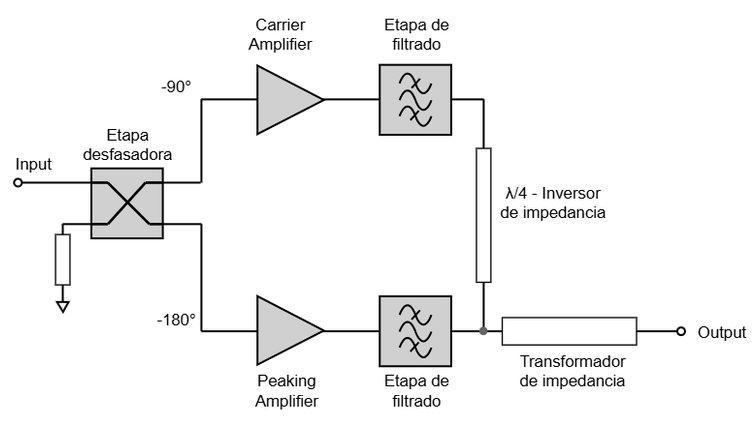
\includegraphics[width=0.7\linewidth]{Figures/doherty.png}
    \caption{Diagrama en bloques de la topología Doherty.}
    \label{fig:doherty_blocks} 
\end{figure}

Los transistores a utilizar para el diseño de los amplificadores son de tecnología GaN. La razón de esta elección es su buen manejo de potencia y linealidad. 

Para diseño, simulación e implementación del PA se utilizarán herramientas como Altium Designer y ANSYS. 
La gestión del proyecto será llevada a cabo empleando la metodología Kanban, empleando Trello, con el objetivo de optimizar y agilizar el flujo de trabajo con el planteo de hitos realizables en el corto plazo.

% -----------------------------------------------------------------------------------------------%
\section{Tema de Investigación}
Como se ha mencionado previamente, en los últimos años los costos asociados al desarrollo y lanzamiento de satélites se han reducido considerablemente gracias al auge de plataformas como los CubeSat. Sin embargo, estos valores continúan siendo significativos. Por esta razón, es indispensable contar con un conocimiento profundo de las posibles fallas y fenómenos adversos que podrían afectar a los sistemas que componen al satélite una vez en órbita. Minimizar estos riesgos es esencial para evitar que una misión fracase y el satélite quede reducido a basura espacial. 

Entre las variables más críticas a considerar en el diseño de sistemas electrónicos para el espacio se encuentra la temperatura. En órbita terrestre baja, los CubeSat se ven expuestos a variaciones térmicas extremas, provocadas principalmente por los ciclos de exposición directa al sol. A esto se suma el hecho de que, en el espacio, no existe la posibilidad de disipar el calor por convección, lo que limita de forma significativa la capacidad de disipación.

En el presente trabajo, el sistema a desarrollar es un amplificador de potencia, el cual constantemente disipa una fracción de la energía que consume en forma de calor. Si no se gestionan adecuadamente estas pérdidas, se corre el riesgo de sobrecalentamiento, lo cual puede provocar desvíos en los parámetros del amplificador e incluso daños permanentes en el dispositivo.

Otra variable fundamental en el entorno espacial es la radiación. Los dispositivos electrónicos a bordo están expuestos a partículas de alta energía, como protones y electrones, además de rayos cósmicos. Esta exposición puede generar efectos acumulativos (TID, Total Ionizing Dose) o eventos puntuales (SEEs, Single Event Effects) que alteren el comportamiento eléctrico de los circuitos. En el caso particular de un PA, se busca estudiar si estos fenómenos podrían inducir variaciones en parámetros críticos como la ganancia, impedancia, eficiencia o punto de compresión.

Frente a estas problemáticas, se plantea como tema de investigación el diseño, desarrollo y caracterización de un amplificador de potencia de alta eficiencia energética, destinado a aplicaciones espaciales, con énfasis en su evaluación ante condiciones adversas. Para ello, el dispositivo será sometido a ensayos que simulen las condiciones reales a las que se enfrentaría en una misión, con el fin de identificar las posibles degradaciones en su rendimiento y establecer criterios de diseño que aseguren su estabilidad y confiabilidad.

Este enfoque permitirá generar conocimientos valiosos en torno al comportamiento de dispositivos de potencia en el espacio y sentar las bases para futuros desarrollos robustos, eficientes y adaptados a las exigencias del entorno. Así, se apunta a contribuir con soluciones tecnológicas viables para plataformas satelitales emergentes, en línea con las crecientes demandas del sector aeroespacial.

\section{Gestión del Alcance}
Para poder llevar a cabo una gestión efectiva del alcance del proyecto se plantearon los objetivos de la Tabla 1. Estos se hallan divididos en cuatro categorías que remarcan su criticidad (a la vez que su factibilidad) dentro del contexto del proyecto. Los objetivos indicados como mandatorios son los que el proyecto debe cumplir obligatoriamente y se considera factible realizar. Los deseables también son considerados como factibles pero no son absolutamente críticos para el éxito del proyecto. Los opcionales son aquellos que harán del proyecto, en caso de cumplirse, un diseño más atractivo pero no están ligados al objetivo principal de este trabajo. Por último, se encuentran los objetivos no incluidos en el proyecto actual.

\begin{table}[H]
    \centering
    \caption{Clasificación de requisitos de diseño del amplificador.}
    \label{tab:requisitos_clasificados}
    \renewcommand{\arraystretch}{1.1}
    \begin{tabular}{cccc}
        \hline\hline
        \textbf{Mandatorios} & \textbf{Deseables} & \textbf{Opcionales} & \textbf{No incluidos} \\
        \hline
        $f_{c} = 2{,}2$ GHz  & OIP3 $\ge 35$ dBm  & Tolerancia a rad.   & ---        \\
        $BW = 35$ MHz        & $BW = 10 \%$       & ---                 & Modulación \\
        $P_{out} \ge 1$ W    & $P_{out} \ge 2$ W  & ---                 & ---        \\
        PAE $\ge 35 \%$      & PAE $\ge 50 \%$    & ---                 & ---        \\
        \hline\hline
    \end{tabular}
\end{table}

\subsection{Hitos}
Una vez definidos los objetivos del proyecto, se establecieron los hitos a partir de los cuales se organiza el trabajo a llevar a cabo. Cada hito representa un fragmento de todo el proyecto y da como resultado, de ser completado satisfactoriamente, un entregable. En la Tabla \ref{tab:mapa_hitos} se muestra cada uno de ellos, junto con su descripción y entregable correspondiente.

\begin{xltabular}{\textwidth}{>{\centering\arraybackslash}p{0.6cm} X X p{2.5cm}}
    \caption{Mapa de hitos del proyecto del amplificador de potencia.} \label{tab:mapa_hitos} \\
    \hline
    \textbf{\#} & \textbf{Hito} & \textbf{Descripción} & \textbf{Entregable} \\
    \hline
    \endfirsthead

    \multicolumn{4}{c}{\textit{Continuación del Cuadro~\ref{tab:mapa_hitos}}} \\
    \hline
    \textbf{\#} & \textbf{Hito} & \textbf{Descripción} & \textbf{Entregable} \\
    \hline
    \endhead

    \hline
    \endfoot

    \hline
    \endlastfoot

    1 & Diseño y simulación clase B y acoplador en ADS & Diseño y simulación en ADS de un amplificador clase B y acoplador. & Archivos de simulación \\
    
    \hline
    2 & Diseño de PCB clase B y acoplador & Incluye revisiones internas. Incluye tener definida la BOM teniendo en cuenta la fabricación en JLCPCB. & Archivos gerber \\
    
    \hline
    3 & Pedido del diseño clase B y acoplador & Realizar el pedido en China. Incluye cargar gerber en JLCPCB, elegir las especificaciones, incluye el sourcing de las partes. & Comprobante de pedido \\
    
    \hline
    4 & Diseño y simulación clase C & Diseño y simulación en ADS de un amplificador clase C. & Archivos de simulación \\
    
    \hline
    5 & Diseño PCB clase C & Incluye revisiones internas. Incluye tener definida la BOM teniendo en cuenta la fabricación en JLCPCB. & Archivos gerber \\
    
    \hline
    6 & PCBs Clase B y acoplador en mano & El día 9 de junio deben haber llegado los PCBs enviados a fabricar y ensamblar en JLCPCB. & PCBs \\
    
    \hline
    7 & Medición y caracterización de los PCBs & Se realizan todas las mediciones necesarias a los PCBs fabricados. & Resultados de medición \\
    
    \hline
    8 & Primera irradiación & Se realizará la irradiación del amplificador clase B y del acoplador. & Foto irradiando \\
    
    \hline
    \rowcolor[HTML]{b6d7a8} \multicolumn{4}{c}{\textbf{Parciales y finales (30/06 a 19/07)}} \\
    
    \hline
    9 & Diseño pasivos Doherty y presentación de resultados de la radiación & Se diseñarán el resto de componentes pasivos de la topología Doherty en ADS. Además se presentarán los resultados de la radiación. & Archivos de simulación y resultados de medición \\
    
    \hline
    10 & Integración del diseño de los pasivos con el amplificador de \textit{peaking} en ADS & Diseño en ADS para integrar los pasivos al amplificador clase C. & Archivos de simulación \\
    
    \hline
    11 & Diseño de PCB del amplificador de \textit{peaking} con sus pasivos & Se realizará el PCB en Altium incluyendo los pasivos en el diseño logrado anteriormente. & Archivos gerber \\
    
    \hline
    12 & Pedido del diseño clase C y red de salida & Realizar el pedido en China. Incluye cargar gerber en JLCPCB, elegir las especificaciones, incluye el \textit{sourcing} de las partes. & Comprobante de pedido \\
    
    \hline
    13 & Simulación en ADS del PCB final, completamente integrado & Diseño en ADS del amplificador Doherty. & Archivos de simulación \\
    
    \hline
    14 & Fabricación de los PCBs de \textit{peaking} y pasivos Doherty & El día X deben haber llegado los PCBs enviados a fabricar y ensamblar en JLCPCB. & PCBs \\
    
    \hline
    15 & Medición y caracterización de los PCBs & Se realizan todas las mediciones necesarias a los PCBs fabricados (en condiciones de realizar pruebas sobre el diseño final). & Resultados de medición \\
    
    \hline
    16 & ADS - Ajuste del diseño del PCB final, completamente integrado & Se ajustan los valores del diseño final en función de las mediciones del amplificador clase C. & Archivos de simulación \\
    
    \hline
    17 & Diseño PCB Doherty & PCB del diseño final. & Archivos gerber \\
    
    \hline
    18 & Pedido del diseño final & Pedido del diseño final en China. & Comprobante de envío \\
    
    \hline
    19 & Tener el PCB del diseño final en mano & Tener el PCB del diseño final en mano habiendo llegado de China. & PCBs \\
    
    \hline
    20 & Medición y caracterización del PCB final & Se realizan todas las mediciones necesarias a los PCBs fabricados del diseño final. & Resultados de medición \\
    
    \hline
    \rowcolor[HTML]{b6d7a8} \multicolumn{4}{c}{\textbf{Baja actividad - Parciales y finales (03/11 a 05/12)}} \\
    
    \hline
    21 & Irradiación del diseño final & Irradiar el diseño final. Probablemente con menor disponibilidad debido a parciales. & Foto irradiando \\
    
    \hline
    22 & Presentación de los resultados de la irradiación & Se presentarán los resultados de la irradiación. & Resultados de medición \\
    
    \hline
    \rowcolor[HTML]{b6d7a8} \multicolumn{4}{c}{\textbf{Fin de diseño y medición}} \\
    
    \hline
    23 & Paper - Trabajo de investigación & Se espera para esta fecha tener la versión final del paper escrita para la publicación definitiva. & Paper \\

    \hline
\end{xltabular}

\subsection{Desglose de Tareas}
Si bien cada hito sirve como un pantallazo general del progreso del proyecto, es imperativo desglosar cada uno de ellos en tareas (y a su vez estas en subtareas) para lograr una división precisa y efectiva del trabajo entre los integrantes del equipo de trabajo. A continuación se muestran las tablas de desglose de tareas para cada hito presentado.

% hito 1
\begin{table}[H]
    \centering
    \renewcommand{\arraystretch}{1.1}
    \begin{tabularx}{\textwidth}{|C{1cm}|C{1.6cm}|Y|Y|}
        \hline
        \multicolumn{4}{|l|}{\textbf{Hito 1 - Diseño Amplificador clase B y acoplador}} \\
        \hline
        \textbf{\#} & \textbf{Subtarea} & \textbf{Título} & \textbf{Descripción} \\ \hline
        1.1 & & Simulación en ADS           & \\ \hline
        1.2 & & Optimización del diseño     & \\ \hline
        1.3 & & Diseño final + simulaciones & \\ \hline
        1.4 & & Revisión interna            & \\
        \hline
    \end{tabularx}
\end{table}

% hito 2
\begin{table}[H]
    \centering
    \renewcommand{\arraystretch}{1.1}
    \begin{tabularx}{\textwidth}{|C{1cm}|C{1.6cm}|Y|Y|}
        \hline
        \multicolumn{4}{|l|}{\textbf{Hito 2 - Diseño de PCB - Clase B y acoplador}} \\
        \hline
        \textbf{\#} & \textbf{Subtarea} & \textbf{Título} & \textbf{Descripción} \\ \hline
        2.1 & & Exportar diseño acoplador            & \\ \hline
        2.2 & & Diseño PCB acoplador                 & \\ \hline
        2.3 & & Esquemático + BOM clase B            & \\ \hline
        2.4 & & Dibujo líneas de transmisión clase B & \\ \hline
        2.5 & & Diseño PCB clase B                   & \\ \hline
        2.6 & & Revisión interna                     & \\
        \hline
    \end{tabularx}
\end{table}

% hito 3
\begin{table}[H]
    \centering
    \renewcommand{\arraystretch}{1.1}
    \begin{tabularx}{\textwidth}{|C{1cm}|C{1.6cm}|Y|Y|}
        \hline
        \multicolumn{4}{|l|}{\textbf{Hito 3 - Pedido del diseño - Clase B y acoplador}} \\
        \hline
        \textbf{\#} & \textbf{Subtarea} & \textbf{Título} & \textbf{Descripción} \\ \hline
        3.1 & & Exportar archivos de fabricación             & \\ \hline
        3.2 & & Definir fabricante y sourcing de componentes & \\ \hline
        3.3 & & Realizar pedido                              & \\
        \hline
    \end{tabularx}
\end{table}

% hito 4
\begin{table}[H]
    \centering
    \renewcommand{\arraystretch}{1.1}
    \begin{tabularx}{\textwidth}{|C{1cm}|C{1.6cm}|Y|Y|}
        \hline
        \multicolumn{4}{|l|}{\textbf{Hito 4 - Diseño y Simulación - Clase C}} \\
        \hline
        \textbf{\#} & \textbf{Subtarea} & \textbf{Título} & \textbf{Descripción} \\ \hline
        4.1 &       & Marco teórico clase C            & \\ \hline
        4.2 &       & Diseño en ADS                    & \\ \cline{2-4}
            & 4.2.1 & Armado del circuito ideal        & Polarización y circuito ideal \\ \cline{2-4}
            & 4.2.2 & Load-pull                        & \\ \cline{2-4}
            & 4.2.3 & Diseño redes de adaptación       & \\ \cline{2-4}
            & 4.2.4 & Optimización redes de adaptación & \\ \cline{2-4}
            & 4.2.5 & Búsqueda de componentes reales   & \\ \cline{2-4}
            & 4.2.6 & Diseño circuito real             & \\ \cline{2-4}
            & 4.2.7 & Optimización circuito real       & \\ \cline{2-4}
            & 4.2.8 & Análisis paramétrico + Robustez  & \\ \hline
        4.3 &       & Revisión interna                 & \\
        \hline
    \end{tabularx}
\end{table}

% hito 5
\begin{table}[H]
    \centering
    \renewcommand{\arraystretch}{1.1}
    \begin{tabularx}{\textwidth}{|C{1cm}|C{1.6cm}|Y|Y|}
        \hline
        \multicolumn{4}{|l|}{\textbf{Hito 5 - Diseño PCB - Clase C}} \\
        \hline
        \textbf{\#} & \textbf{Subtarea} & \textbf{Título} & \textbf{Descripción} \\ \hline
        5.1 &        & Diseño esquemático                  & \\ \cline{2-4}
            & 5.1.1  & Dibujo del circuito simulado en ADS & \\ \cline{2-4}
            & 5.1.2  & Asignación de footprints            & \\ \hline
        5.2 &        & Armado BOM & Excel con part numbers de todos los componentes \\ \hline
        5.3 &        & Diseño PCB                          & \\ \cline{2-4}
            & 5.3.1  & Placement de componentes & Definición boardshape y placement \\ \cline{2-4}
            & 5.3.2  & Dibujo líneas de transmisión        & \\ \cline{2-4}
            & 5.3.3  & Completar PCB                       & \\ \hline
        5.4 &        & Revisión interna                    & \\
        \hline
    \end{tabularx}
\end{table}

% hito 6
\begin{table}[H]
    \centering
    \renewcommand{\arraystretch}{1.1}
    \begin{tabularx}{\textwidth}{|C{1cm}|C{1.6cm}|Y|Y|}
        \hline
        \multicolumn{4}{|l|}{\textbf{Hito 6 - Tener los PCBs Clase B y acoplador en mano}} \\
        \hline
        \textbf{\#} & \textbf{Subtarea} & \textbf{Título} & \textbf{Descripción} \\ \hline
        6.1 & & Llevar y retirar los PCBs en Outsource para ensamblaje & \\
        \hline
    \end{tabularx}
\end{table}

% hito 7
\begin{table}[H]
    \centering
    \renewcommand{\arraystretch}{1.1}
    \begin{tabularx}{\textwidth}{|C{1cm}|C{1.6cm}|Y|Y|}
        \hline
        \multicolumn{4}{|l|}{\textbf{Hito 7 - Medición y caracterización de los PCBs}} \\
        \hline
        \textbf{\#} & \textbf{Subtarea} & \textbf{Título} & \textbf{Descripción} \\ \hline
        7.1 & 7.1.1 & Coordinación fecha grupo & \\ \cline{2-4}
            & 7.1.2 & Coordinación con tutor   & Hablar con un tutor para que nos asista con las mediciones (Carlos Navarro, Manuel García, Alejandro Henze, Matías Hampel) \\ \hline
        7.2 &       & Reserva del laboratorio y equipos & \\ \hline
        7.3 &       & Planeamiento del experimento      & \\ \hline
        7.4 &       & Mediciones                        & \\ \hline
        7.5 &       & Informe interno & Análisis de resultados y presentación informe interno \\
        \hline
    \end{tabularx}
\end{table}

% hito 8
\begin{table}[H]
    \centering
    \renewcommand{\arraystretch}{1.1}
    \begin{tabularx}{\textwidth}{|C{1cm}|C{1.6cm}|Y|Y|}
        \hline
        \multicolumn{4}{|l|}{\textbf{Hito 8 - Primera Irradiación}} \\
        \hline
        \textbf{\#} & \textbf{Subtarea} & \textbf{Título} & \textbf{Descripción} \\ \hline
        8.1 & & Marco teórico irradiación        & \\ \hline
        8.2 & & Definir experimento a realizar   & \\ \hline
        8.3 & & Pedido de turno                  & \\ \hline
        8.4 & & Preparar instrumental necesario  & Solicitar instrumental en caso de ser necesario \\ \hline
        8.5 & & Medición                         & \\
        \hline
    \end{tabularx}
\end{table}

% hito 9
\begin{table}[H]
    \centering
    \renewcommand{\arraystretch}{1.1}
    \begin{tabularx}{\textwidth}{|C{1cm}|C{1.6cm}|Y|Y|}
        \hline
        \multicolumn{4}{|l|}{\textbf{Hito 9 - Diseño Pasivos Doherty y Resultados de Radiación}} \\
        \hline
        \textbf{\#} & \textbf{Subtarea} & \textbf{Título} & \textbf{Descripción} \\ \hline
        9.1 &       & Análisis de resultados                   & Informe explicando lo que se obtuvo del experimento \\ \hline
        9.2 &       & Diseño de pasivos en ADS                 & \\ \hline
            & 9.2.1 & Armado de circuito ideal                 & \\ \hline
            & 9.2.2 & Simulación y análisis del circuito ideal & \\ \hline
            & 9.2.3 & Armado de circuito real                  & \\ \hline
            & 9.2.4 & Simulación y análisis del circuito real  & \\ \hline
            & 9.2.5 & Optimización                             & \\ \hline
            & 9.2.6 & Simulación EM                            & \\ \hline
        9.3 &       & Revisión interna                         & \\ \hline
        9.4 &       & Simulación EM con ANSYS o CST            & \\
        \hline
    \end{tabularx}
\end{table}

% hito 10
\begin{table}[H]
    \centering
    \renewcommand{\arraystretch}{1.1}
    \begin{tabularx}{\textwidth}{|C{1cm}|C{1.6cm}|Y|Y|}
        \hline
        \multicolumn{4}{|l|}{\textbf{Hito 10 - Integración del diseño de pasivos con clase C en ADS}} \\
        \hline
        \textbf{\#} & \textbf{Subtarea} & \textbf{Título} & \textbf{Descripción} \\ \hline
        10.1 & & Simulación pasivos + clase C & \\ \hline
        10.2 & & Optimización                 & \\ \hline
        10.3 & & Revisión interna             & \\
        \hline
    \end{tabularx}
\end{table}

% hito 11
\begin{table}[H]
    \centering
    \renewcommand{\arraystretch}{1.1}
    \begin{tabularx}{\textwidth}{|C{1cm}|C{1.6cm}|Y|Y|}
        \hline
        \multicolumn{4}{|l|}{\textbf{Hito 11 - Diseño PCB amplificador clase C con pasivos}} \\
        \hline
        \textbf{\#} & \textbf{Subtarea} & \textbf{Título} & \textbf{Descripción} \\ \hline
        11.1 &         & Diseño esquemático                  & \\ \cline{2-4}
             & 11.1.1  & Dibujo del circuito simulado en ADS & \\ \cline{2-4}
             & 11.1.2  & Asignación de footprints            & \\ \hline
        11.2 &         & Armado BOM & Excel con part numbers de todos los componentes \\ \hline
        11.3 &         & Diseño PCB                          & \\ \cline{2-4}
             & 11.3.1  & Placement de componentes            & \\ \cline{2-4}
             & 11.3.2  & Dibujo líneas de transmisión        & \\ \cline{2-4}
             & 11.3.3  & Completar PCB                       & \\ \hline
        11.4 &         & Revisión interna                    & \\
        \hline
    \end{tabularx}
\end{table}

% hito 12
\begin{table}[H]
    \centering
    \renewcommand{\arraystretch}{1.1}
    \begin{tabularx}{\textwidth}{|C{1cm}|C{1.6cm}|Y|Y|}
        \hline
        \multicolumn{4}{|l|}{\textbf{Hito 12 - Pedido del diseño clase C y pasivos}} \\
        \hline
        \textbf{\#} & \textbf{Subtarea} & \textbf{Título} & \textbf{Descripción} \\ \hline
        12.1 & & Exportar archivos de fabricación             & Gerber y drill \\ \hline
        12.2 & & Definir fabricante y sourcing de componentes & \\ \hline
        12.3 & & Realizar pedido                              & \\
        \hline
    \end{tabularx}
\end{table}

% hito 13
\begin{table}[H]
    \centering
    \renewcommand{\arraystretch}{1.1}
    \begin{tabularx}{\textwidth}{|C{1cm}|C{1.6cm}|Y|Y|}
        \hline
        \multicolumn{4}{|l|}{\textbf{Hito 13 - Simulación en ADS del PCB final}} \\
        \hline
        \textbf{\#} & \textbf{Subtarea} & \textbf{Título} & \textbf{Descripción} \\ \hline
        13.1 &         & Pensar el diseño                  & \\ \hline
        13.2 &         & Diseño en ADS                     & \\ \cline{2-4}
             & 13.2.1  & Armado circuito ideal             & Polarización y circuito ideal \\ \cline{2-4}
             & 13.2.2  & Optimización redes de adaptación  & \\ \cline{2-4}
             & 13.2.3  & Búsqueda de componentes reales    & \\ \cline{2-4}
             & 13.2.4  & Diseño circuito real              & \\ \cline{2-4}
             & 13.2.5  & Optimización circuito real        & \\ \cline{2-4}
             & 13.2.6  & Análisis paramétrico + robustez   & \\ \hline
        13.3 &         & Revisión interna                  & \\
        \hline
    \end{tabularx}
\end{table}

% hito 14
\begin{table}[H]
    \centering
    \renewcommand{\arraystretch}{1.1}
    \begin{tabularx}{\textwidth}{|C{1cm}|C{1.6cm}|Y|Y|}
        \hline
        \multicolumn{4}{|l|}{\textbf{Hito 14 - Fabricación de los PCBs peaking y pasivos Doherty}} \\
        \hline
        \textbf{\#} & \textbf{Subtarea} & \textbf{Título} & \textbf{Descripción} \\ \hline
        14.1 & & Llevar y retirar los PCBs en Outsource para ensamblaje & \\
        \hline
    \end{tabularx}
\end{table}

% hito 15
\begin{table}[H]
    \centering
    \renewcommand{\arraystretch}{1.1}
    \begin{tabularx}{\textwidth}{|C{1cm}|C{1.6cm}|Y|Y|}
        \hline
        \multicolumn{4}{|l|}{\textbf{Hito 15 - Medición y caracterización de los PCBs}} \\
        \hline
        \textbf{\#} & \textbf{Subtarea} & \textbf{Título} & \textbf{Descripción} \\ \hline
        15.1 & 15.1.1 & Coordinación fecha           & \\ \cline{2-4}
             & 15.1.2 & Coordinación con tutor       & \\ \hline
        15.2 &        & Reserva del laboratorio y equipos & \\ \hline
        15.3 &        & Planeamiento del experimento      & \\ \hline
        15.4 &        & Mediciones                        & \\ \hline
        15.5 &        & Informe interno & Análisis de resultados y presentación informe interno \\
        \hline
    \end{tabularx}
\end{table}

% hito 16
\begin{table}[H]
    \centering
    \renewcommand{\arraystretch}{1.1}
    \begin{tabularx}{\textwidth}{|C{1cm}|C{1.6cm}|Y|Y|}
        \hline
        \multicolumn{4}{|l|}{\textbf{Hito 16 - ADS. Ajuste del diseño del PCB final}} \\
        \hline
        \textbf{\#} & \textbf{Subtarea} & \textbf{Título} & \textbf{Descripción} \\ \hline
        16.1 & 16.1.1 & Análisis del circuito real a partir de valores obtenidos en el clase C & \\ \cline{2-4}
             & 16.1.2 & Optimización del circuito real  & \\ \cline{2-4}
             & 16.1.3 & Análisis paramétrico + robustez & \\ \hline
        16.2 &        & Revisión interna                & \\
        \hline
    \end{tabularx}
\end{table}

% hito 17
\begin{table}[H]
    \centering
    \renewcommand{\arraystretch}{1.1}
    \begin{tabularx}{\textwidth}{|C{1cm}|C{1.6cm}|Y|Y|}
        \hline
        \multicolumn{4}{|l|}{\textbf{Hito 17 - Diseño PCB Doherty}} \\
        \hline
        \textbf{\#} & \textbf{Subtarea} & \textbf{Título} & \textbf{Descripción} \\ \hline
        17.1 &         & Diseño esquemático                  & \\ \cline{2-4}
             & 17.1.1  & Dibujo del circuito simulado en ADS & \\ \cline{2-4}
             & 17.1.2  & Asignación de footprints            & \\ \hline
        17.2 &         & Armado BOM                          & \\ \hline
        17.3 &         & Diseño PCB                          & \\ \cline{2-4}
             & 17.3.1  & Placement de componentes            & \\ \cline{2-4}
             & 17.3.2  & Dibujo líneas de transmisión        & \\ \cline{2-4}
             & 17.3.3  & Completar PCB                       & \\ \hline
        17.4 &         & Revisión interna                    & \\
        \hline
    \end{tabularx}
\end{table}

% hito 18
\begin{table}[H]
    \centering
    \renewcommand{\arraystretch}{1.1}
    \begin{tabularx}{\textwidth}{|C{1cm}|C{1.6cm}|Y|Y|}
        \hline
        \multicolumn{4}{|l|}{\textbf{Hito 18 - Pedido del diseño final}} \\
        \hline
        \textbf{\#} & \textbf{Subtarea} & \textbf{Título} & \textbf{Descripción} \\ \hline
        18.1 & & Exportar archivos de fabricación             & Gerber y drill \\ \hline
        18.2 & & Definir fabricante y sourcing de componentes & \\ \hline
        18.3 & & Realizar pedido                              & \\
        \hline
    \end{tabularx}
\end{table}

% hito 19
\begin{table}[H]
    \centering
    \renewcommand{\arraystretch}{1.1}
    \begin{tabularx}{\textwidth}{|C{1cm}|C{1.6cm}|Y|Y|}
        \hline
        \multicolumn{4}{|l|}{\textbf{Hito 19 - PCB final en mano}} \\
        \hline
        \textbf{\#} & \textbf{Subtarea} & \textbf{Título} & \textbf{Descripción} \\ \hline
        19.1 & & Llevar y retirar los PCBs en Outsource para ensamblaje & \\
        \hline
    \end{tabularx}
\end{table}

% hito 20
\begin{table}[H]
    \centering
    \renewcommand{\arraystretch}{1.1}
    \begin{tabularx}{\textwidth}{|C{1cm}|C{1.6cm}|Y|Y|}
        \hline
        \multicolumn{4}{|l|}{\textbf{Hito 20 - Medición y caracterización PCB final}} \\
        \hline
        \textbf{\#} & \textbf{Subtarea} & \textbf{Título} & \textbf{Descripción} \\ \hline
        20.1 & 20.1.1 & Coordinación fecha grupo & \\ \cline{2-4}
             & 20.1.2 & Coordinación con tutor   & Hablar con un tutor para que nos asista con las mediciones (Carlos Navarro, Manuel García, Alejandro Henze, Matías Hampel) \\ \hline
        20.2 &        & Reserva del laboratorio y equipos & \\ \hline
        20.3 &        & Planeamiento del experimento      & \\ \hline
        20.4 &        & Mediciones                        & \\ \hline
        20.5 &        & Informe interno & Análisis de resultados y presentación informe interno \\
        \hline
    \end{tabularx}
\end{table}

% hito 21
\begin{table}[H]
    \centering
    \renewcommand{\arraystretch}{1.1}
    \begin{tabularx}{\textwidth}{|C{1cm}|C{1.6cm}|Y|Y|}
        \hline
        \multicolumn{4}{|l|}{\textbf{Hito 21 - Irradiación del diseño final}} \\
        \hline
        \textbf{\#} & \textbf{Subtarea} & \textbf{Título} & \textbf{Descripción} \\ \hline
        21.1 & & Marco teórico irradiación      & \\ \hline
        21.2 & & Definir experimento a realizar & \\ \hline
        21.3 & & Pedido de turno                & \\ \hline
        21.4 & & Preparar instrumental          & Solicitar instrumental en caso de ser necesario \\ \hline
        21.5 & & Medición                       & \\
        \hline
    \end{tabularx}
\end{table}

% hito 22
\begin{table}[H]
    \centering
    \renewcommand{\arraystretch}{1.1}
    \begin{tabularx}{\textwidth}{|C{1cm}|C{1.6cm}|Y|Y|}
        \hline
        \multicolumn{4}{|l|}{\textbf{Hito 22 - Presentación resultados de irradiación}} \\
        \hline
        \textbf{\#} & \textbf{Subtarea} & \textbf{Título} & \textbf{Descripción} \\ \hline
        22.1 & & Análisis de resultados & Informe explicando lo obtenido del experimento \\
        \hline
    \end{tabularx}
\end{table}

% hito 23
\begin{table}[H]
    \centering
    \renewcommand{\arraystretch}{1.1}
    \begin{tabularx}{\textwidth}{|C{1cm}|C{1.6cm}|Y|Y|}
        \hline
        \multicolumn{4}{|l|}{\textbf{Hito 23 - Paper}} \\
        \hline
        \textbf{\#} & \textbf{Subtarea} & \textbf{Título} & \textbf{Descripción} \\ \hline
        23.1 & & Preparación marco teórico          & Búsqueda de referencias y papers \\ \hline
        23.2 & & Pensar qué decir y cómo            & \\ \hline
        23.3 & & Armar el esqueleto del paper       & \\ \hline
        23.4 & & Escribir el abstract               & \\ \hline
        23.5 & & Escribir las secciones             & \\ \hline
        23.6 & & Revisión por parte de otros grupos & \\ \hline
        23.7 & & Revisión por tutores docentes      & \\ \hline
        23.8 & & Publicación                        & \\
        \hline
    \end{tabularx}
\end{table}

\section{Gestión del Tiempo}
Un diagrama Gantt fue realizado para gestionar el tiempo del proyecto. Mediante el uso de este diagrama es posible determinar la factibilidad del desarrollo del proyecto dentro del tiempo establecido y, simultáneamente, identificar cuellos de botella, tareas que sea posible (o no) paralelizar y gestionar de mejor manera el tiempo de cada tarea.

El proyecto consta de varias etapas, algunas superpuestas temporalmente con otras. Tanto las etapas como su paralelización, en caso de haber, se ilustran en la Figura 2.

\section{Gestión del Riesgo}
La realización de una matriz de riesgos resultó importante para tener una visualización de todos los riesgos existentes a la vez que una ponderación de la relevancia de los mismos. 

Para hacer esto, a cada riesgo considerado se le asignó una probabilidad de ocurrencia y una magnitud al impacto del evento sobre el proyecto. En base a estos dos indicadores, se otorga al evento una calificación, la cual indica que tan importante es el atacar ese problema.

La probabilidad de ocurrencia se mide de 0 a 1, mientras que la magnitud podrá ser muy bajo, bajo, medio, alto y muy alto. A mayor probabilidad de ocurrencia y mayor magnitud de impacto mayor es la calificación que se le otorga al evento. Dicha calificación podrá ser bajo, medio, alto y muy alto. A continuación, la tabla con los eventos.

\small
\renewcommand{\arraystretch}{1.15}

\newcommand{\bajo}{\cellcolor{yellow!20}BAJO}
\newcommand{\medio}{\cellcolor{orange!25}MEDIO}
\newcommand{\alto}{\cellcolor{red!20}ALTO}
\newcommand{\muyalto}{\cellcolor{red!45}\textbf{MUY ALTO}}

\begin{xltabular}{\textwidth}{|>{\centering\arraybackslash}p{0.7cm}|p{4.0cm}|p{1.3cm}|p{1.2cm}|>{\centering\arraybackslash}p{0.8cm}|p{1.2cm}|}

\caption{Matriz de riesgos del proyecto.} \label{tab:risk_matrix} \\

\hline
\textbf{EDT} & \textbf{Descripción del evento de riesgo} & \textbf{Fuente} & \textbf{Imp.} & \textbf{Prob.} & \textbf{Calif.} \\
\hline
\endfirsthead

\multicolumn{4}{c}{\textit{Continuación del Cuadro~\ref{tab:mapa_hitos}}} \\
\hline
\textbf{EDT} & \textbf{Descripción del evento de riesgo} & \textbf{Fuente} & \textbf{Imp.} & \textbf{Prob.} & \textbf{Calif.} \\
\hline
\endhead

\hline
\endfoot

\hline
\endlastfoot

\multirow{2}{*}{3.2} & El sourcing de componentes se encuentra en un lugar diferente al ensamblaje. Pueden producirse tiempos y costos extras. & Logística & Medio & 0.7 & \alto \\ \cline{2-6}
& Es posible que Outsource no esté disponible. & Logística & Medio & 0.5 & \medio \\ \hline
3.3 & Costos extras de aduana. & Econ. & Muy bajo & 0.8 & \bajo \\ \hline

4.2.1 & No se puede realizar un buen análisis de estabilidad y el circuito puede volverse inestable. & Técnico & Alto & 0.2 & \medio \\ \hline
4.2.5 & No existan componentes adecuados. & Tecnol. & Bajo & 0.2 & \bajo \\ \hline
4.2.8 & Que resulte un circuito poco robusto. & Técnico & Medio & 0.25 & \bajo \\ \hline

5.1.2 & Error en la asignación de algún footprint. & Operativo & Alto & 0.2 & \medio \\ \hline

6.1 & Es posible que Outsource no esté disponible. & Logística & Medio & 0.5 & \medio \\ \hline

\multirow{2}{*}{7.4} & Mediciones que no dan bien. & Técnico & Alto & 0.3 & \alto \\ \cline{2-6}
& Destrucción del dispositivo por alta potencia manejada. & Técnico & Muy Alto & 0.1 & \medio \\ \hline

\multirow{2}{*}{8.3} & Demora en la asignación de turno. & Operativo & Bajo & 0.4 & \bajo \\ \cline{2-6}
& Indisponibilidad del experimento. & Operativo & Alto & 0.1 & \bajo \\ \hline
8.4 & Indisponibilidad del instrumental. & Operativo & Alto & 0.2 & \medio \\ \hline

9.1 & Obtención de resultados no significativos. & Técnico & Medio & 0.5 & \medio \\ \hline

10.1 & Integración fallida. Se deberá rediseñar. & Técnico & Medio & 0.25 & \bajo \\ \hline

11.1.2 & Error en la asignación de algún footprint. & Operativo & Alto & 0.1 & \bajo \\ \hline

\multirow{2}{*}{12.2} & El sourcing de componentes se encuentra en un lugar diferente al ensamblaje. Pueden producirse tiempos y costos extras. & Logística & Medio & 0.7 & \alto \\ \cline{2-6}
& Es posible que Outsource no esté disponible. & Logística & Medio & 0.5 & \medio \\ \hline
12.3 & Costos extras de aduana. & Econ. & Muy bajo & 0.8 & \bajo \\ \hline

13.2.4 & Imposibilidad de integrar el diseño de un amplificador Doherty. & Técnico & Medio & 0.5 & \bajo \\ \hline
13.2.6 & Que resulte un circuito poco robusto. & Técnico & Medio & 0.25 & \bajo \\ \hline

14.1 & Es posible que Outsource no esté disponible. & Logística & Medio & 0.5 & \medio \\ \hline

15.4 & Mediciones que no dan bien. & Técnico & Alto & 0.3 & \medio \\ \hline

16.2.3 & Diseño final poco robusto. & Técnico & Medio & 0.5 & \medio \\ \hline

\multirow{2}{*}{18.2} & El sourcing de componentes se encuentra en un lugar diferente al ensamblaje. Pueden producirse tiempos y costos extras. & Logística & Bajo & 0.7 & \medio \\ \cline{2-6}
& Es posible que Outsource no esté disponible. & Logística & Bajo & 0.5 & \bajo \\ \hline
18.3 & Costos extras de aduana. & Econ. & Muy bajo & 0.8 & \bajo \\ \hline

19.1 & Es posible que Outsource no esté disponible. & Logística & Bajo & 0.6 & \bajo \\ \hline

20.4 & Mediciones que no dan bien en el diseño final. & Técnico & Bajo & 0.5 & \bajo \\ \hline

21.2 & Es posible que el PCB final exceda el tamaño máximo del experimento. & Operativo & Medio & 0.5 & \medio \\ \hline
21.4 & Indisponibilidad del instrumental. & Operativo & Medio & 0.25 & \bajo \\ \hline

22.1 & Obtención de resultados no significativos. & Técnico & Alto & 0.75 & \muyalto \\ \hline

23.8 & Paper rechazado. & Tecnol. & Muy Alto & 0.5 & \alto \\ \hline

\end{xltabular}

El análisis de las estrategias a tomar ante los riesgos fue realizado una vez que se habían enviado a ensamblar las placas del amplificador de carrier y donde nos disponíamos a realizar las mediciones, es decir en el hito número 7. Es por eso que se plantearon estrategias a partir de este punto. 
Las estrategias se enfocan en los eventos de impacto medio y alto en el proyecto, ya que son éstos los que tendrán un efecto mayor en el éxito del proyecto.

Por último, cabe destacar que luego de realizado el presente análisis de riesgo, se midió la placa del amplificador de carrier, la cual dio dentro de los valores esperados. Éste amplificador cumple con los objetivos mínimos del proyecto, lo que tiene como consecuencia una reducción generalizada del riesgo del proyecto.

\section{Gestión de Calidad}
En pos de poder visualizar rápidamente el cumplimiento de tiempos y objetivos del proyecto, resulta pertinente emplear un método para la gestión de calidad del mismo. Se implementará un sistema de indicadores los cuales revelarán, de manera cuantitativa, el estado de cada una de las partes claves del proyecto. Los indicadores se dividen en dos categorías: por un lado, aquellos asociados a parámetros del hardware desarrollado, por el otro, los relacionados a la planificación y gestión del proyecto.

En pos de poder visualizar rápidamente el cumplimiento de tiempos y objetivos del proyecto, resulta pertinente emplear un método para la gestión de calidad del mismo. Se implementará un sistema de indicadores los cuales revelarán, de manera cuantitativa, el estado de cada una de las partes claves del proyecto. Los indicadores se dividen en dos categorías: por un lado, aquellos asociados a parámetros del hardware desarrollado, por el otro, los relacionados a la planificación y gestión del proyecto.

\textbf{Indicadores de Hardware}
\begin{itemize}
    \item \textbf{Máxima potencia de salida.} Fuente: ensayos de laboratorio Indica la potencia máxima que el amplificador puede entregar sin comprometer la integridad del PCB ni degradar otros parámetros del amplificador.
    \item \textbf{Ganancia del amplificador.} Fuente: ensayos de laboratorio. Indica el cociente entre potencia de salida y potencia inyectada a la entrada.
    \item \textbf{Eficiencia del amplificador.} Fuente: ensayos de laboratorio. Cociente entre la potencia de salida y la potencia total consumida para obtener esa señal de salida.
    \item \textbf{Desviación de la frecuencia central.} Fuente: ensayos de laboratorio. Indica, de manera porcentual, el corrimiento de la frecuencia central real respecto de la prevista (2,2 GHz).
    \item \textbf{Linealidad (o distorsión) de la señal de salida.} Fuente: ensayos de laboratorio. Evalúa la fidelidad de la señal amplificada, útil para determinar la viabilidad de uso de modulaciones de ciertas modulaciones complejas (QAM). Se medirá a través de parámetros como el punto de intercepción de tercer orden (OIP3) y la distorsión armónica total (THD).
    \item \textbf{Área ocupada por el PCB.} Fuente: diseño CAD. Siendo la placa parte de un CubeSat, cuyo espacio es limitado, se evaluará el área total ocupada por el PCB.
\end{itemize}

\textbf{Indicadores del Proyecto}
\begin{itemize}
    \item \textbf{Retraso respecto del Gantt.} Medido como la diferencia entre tareas efectivamente completadas y tareas planificadas para una determinada fecha.
    \item \textbf{Porcentaje de entregables cumplidos.} Indica cuántos entregables han sido completados satisfactoriamente en relación al total. Refleja el grado de avance del proyecto.
    \item \textbf{Cantidad de iteraciones de diseño.} Indica la cantidad de ciclos de diseño, prueba y ajuste que fueron necesarios para alcanzar los objetivos y parámetros deseados. Da una representación de la eficiencia del proceso de diseño.
\end{itemize}


\chapter{Redefinición del Alcance y Objetivos del Proyecto} \label{sec:alcance}
Durante el transcurso del proyecto se identificaron una serie de restricciones de carácter económico, logístico y operativo que, en conjunto, tornaron inviable la ejecución del plan original en su totalidad. A continuación se describen los factores determinantes que motivaron la redefinición del alcance.

El plan original contempló el desarrollo de tres diseños de circuito impreso distintos: el amplificador de operación permanente en Clase AB, el amplificador de cresta en Clase C y los elementos pasivos de la topología Doherty. El costo unitario del transistor empleado, sumado a los costos de fabricación, envío y ensamblado de cada iteración de placa, representó una restricción económica significativa. Si bien las demoras asociadas al proceso de fabricación y envío desde el exterior fueron contempladas en la planificación original, la acumulación de estos tiempos a lo largo de tres iteraciones de fabricación habría comprometido seriamente el cronograma del proyecto. Adicionalmente, el ensamblado del primer circuito impreso fue realizado sin costo por parte de la empresa Outsource, beneficio que no podía garantizarse para las iteraciones subsiguientes, lo que introdujo una incertidumbre adicional tanto en los costos como en los plazos.

Desde el punto de vista del acceso a equipamiento de medición, el departamento de ingeniería electrónica de la facultad presentó limitaciones tanto de alcance como de funcionamiento de su instrumental disponible para la caracterización de circuitos de radiofrecuencia a las frecuencias de trabajo consideradas en este proyecto. Por un lado, el analizador de espectro de mayor rango disponible en la facultad alcanza una frecuencia máxima de 3~GHz, insuficiente para la medición del contenido armónico del amplificador, dado que el tercer armónico de la frecuencia de operación se ubica en 6,6~GHz, fuera del rango de dicho instrumento. Por otro lado, se detectó durante las primeras sesiones de medición que el tono generado a la salida del generador de señales de RF disponible no coincidía con la frecuencia indicada en el equipo, lo que comprometió adicionalmente la posibilidad de realizar mediciones confiables con el equipamiento propio de la institución. Para subsanar estas limitaciones se recurrió a la Comisión Nacional de Energía Atómica (CNEA) y a la Universidad Nacional de San Martín (UNSAM), instituciones donde finalmente se llevaron a cabo las mediciones. Sin embargo, el acceso a los equipos y a la ayuda por parte del personal en dichas instituciones requirió coordinación anticipada y estuvo sujeto a la disponibilidad tanto de los integrantes del grupo como de las propias instituciones, lo que limitó no solo la frecuencia con que pudieron realizarse sesiones de medición, sino también el tiempo disponible dentro de cada sesión, dado que los equipos y los espacios de trabajo debieron compartirse con otras actividades propias de cada institución. Extender este esquema a la caracterización de tres diseños distintos habría requerido una cantidad y duración de sesiones de medición difícilmente compatible con los plazos disponibles.

En relación con los ensayos de irradiación contemplados en el anteproyecto, se presentaron dificultades para dar con una instalación experimental disponible cuyo tamaño de muestra admisible fuera compatible con las dimensiones del primer circuito impreso fabricado. Esta incompatibilidad física, sumada a la complejidad logística asociada a la coordinación de turnos de irradiación, llevó a desestimar la realización de este ensayo dentro del alcance del presente trabajo.

Frente a este conjunto de restricciones, y considerando que los resultados obtenidos en la caracterización del amplificador Clase AB, satisficieron en gran medida los objetivos de prestaciones establecidos en el anteproyecto, se tomó la decisión de redefinir el alcance del proyecto. El desarrollo quedó acotado al amplificador de potencia en Clase AB y al acoplador híbrido en cuadratura. El amplificador Clase AB constituyó por sí mismo un amplificador de potencia funcional que cumplió con gran parte de los requisitos de la misión, mientras que el acoplador híbrido representó una primera instancia de desarrollo que sentó las bases para una eventual continuación del trabajo hacia la implementación completa de la topología Doherty en el futuro. El ensayo de irradiación fue excluido del alcance actual, redirigiendo los esfuerzos hacia una caracterización experimental más exhaustiva de los parámetros del amplificador fabricado.
\include{Chapters/03-CubeSatLEO.tex}
\include{Chapters/04-PowerAmps.tex}
\include{Chapters/05-GaN.tex}
\include{Chapters/06-Acopladores.tex}
\chapter[Solución propuesta]{Solución Propuesta} \label{sec:solucion_propuesta}
A partir del marco teórico desarrollado en los capítulos anteriores, en particular del análisis de acopladores direccionales del Capítulo~\ref{cp:introduction}, de los criterios de diseño de amplificadores de potencia discutidos en el Capítulo~\ref{sec:teoria_pa} y del análisis comparativo de tecnologías semiconductoras del Capítulo~\ref{sec:gan_hemt} se desarrollaron dos circuitos de radiofrecuencia para el subsistema de comunicaciones en banda S de la misión CubeSat, un acoplador híbrido en cuadratura y un amplificador de potencia monoetapa basado en el transistor GaN HEMT CGH40006S~\cite{macom}, polarizado en Clase AB.

De acuerdo con el Reglamento de Radiocomunicaciones de la Unión Internacional de Telecomunicaciones \cite{itu2024}, el rango de 2170~MHz a 2200~MHz se asigna al Servicio Móvil por Satélite (MSS) para enlaces de bajada, mientras que el intervalo de 2200~MHz a 2290~MHz se destina a la investigación espacial. Operar en torno a 2200~MHz resulta provechoso al encontrarse en la proximidad de ambas bandas, lo que permite mantener compatibilidad espectral con sistemas MSS y a su vez alinearse con las frecuencias utilizadas en misiones de exploración e investigación espacial. Por este motivo, se estableció la frecuencia de portadora de 2,2~GHz como frecuencia de operación tanto del acoplador como del amplificador desarrollados.

El desarrollo de ambos circuitos siguió una misma metodología de trabajo, estructurada en tres etapas sucesivas, a saber, el diseño y la simulación del circuito empleando un software especializado, el diseño del circuito impreso correspondiente y su fabricación, y la caracterización experimental del prototipo resultante mediante un conjunto de mediciones de laboratorio. Dado que esta metodología resulta común a ambos desarrollos, con la salvedad de las particularidades propias del comportamiento pasivo del acoplador frente al comportamiento activo y no lineal del amplificador, se la describe de manera conjunta en las secciones siguientes, antes de abordar el proceso de diseño específico de cada circuito.

Las Secciones~\ref{sec:diseno_acoplador} y~\ref{sec:diseno_amplificador} desarrollan, respectivamente, el diseño del acoplador híbrido y el diseño del amplificador de potencia, incluyendo en este último caso el análisis de radioenlace satelital que determinó la potencia de salida y el esquema de modulación objetivo de la misión. Los resultados de la caracterización experimental de ambos prototipos se presentan en el Capítulo~\ref{sec:resultados}.

% -----------------------------------------------------------------------------------------------%
\section{Metodología de diseño y simulación} \label{sec:metodologia_diseno_sim}
El diseño y la simulación de ambos circuitos se realizaron mediante el entorno Advanced Design System (ADS) de Keysight, empleando bibliotecas de modelos para componentes reales de montaje superficial (SMD) provista por los fabricantes correspondientes, en lugar de modelos ideales de elementos discretos. Sobre el esquemático de simulación de cada circuito se ejecutaron rutinas de optimización numérica para ajustar las dimensiones de las líneas de transmisión que conforman las redes de adaptación y de acoplamiento, hasta alcanzar las condiciones de desempeño requeridas en la frecuencia de operación. Adicionalmente, en los casos en que el circuito requería capacitores o inductores discretos, se realizó una optimización sobre el valor de dichos componentes, en la cual el optimizador recorrió el conjunto de valores disponibles en la biblioteca de componentes reales para el capacitor o el inductor correspondiente, en lugar de optimizar un valor continuo de capacitancia o inductancia sin restricción, de modo de obtener directamente un diseño realizable.

Adicionalmente, en el caso particular del acoplador, se empleó simulación electromagnética de onda completa para verificar el comportamiento del layout de PCB una vez finalizado su diseño, mediante los entornos High Frequency Structure Simulator (HFSS) de Ansys y CST Studio Suite de Dassault Systèmes~\cite{cst}. Ambas herramientas se emplearon de manera comparativa entre sí, mientras que los resultados obtenidos en CST fueron los adoptados como referencia para la comparación con las mediciones experimentales presentada en el Capítulo~\ref{sec:resultados}.

El conjunto específico de simulaciones realizadas sobre cada circuito difirió de acuerdo con su naturaleza. En el caso del acoplador, un circuito pasivo y lineal, la caracterización se realizó fundamentalmente mediante la simulación de parámetros S a nivel de esquemático y mediante la simulación electromagnética de onda completa del layout descripta en el párrafo anterior. En el caso del amplificador, un circuito activo y no lineal, se incorporaron en cambio simulaciones de estabilidad, de load-pull, de balance armónico y de transitorio en el dominio temporal, orientadas a caracterizar su comportamiento de gran señal, sin recurrir a simulación electromagnética de onda completa. Estas simulaciones adicionales, así como su fundamento, se describen en la Sección~\ref{sec:diseno_amplificador}.

% -----------------------------------------------------------------------------------------------%
\section{Metodología de diseño de PCB} \label{sec:metodologia_pcb}
El diseño del circuito impreso (PCB) de ambos desarrollos se realizó en el entorno Altium Designer, a partir de los modelos de las líneas de transmisión previamente dimensionadas y optimizadas en ADS, los cuales se exportaron y trasladaron al layout de la placa. Sobre dicho layout se incorporaron las vías de masa requeridas para garantizar la continuidad del plano de referencia y se configuró la estructura de capas (stackup) de la placa de acuerdo con el proceso de fabricación JLC04161H-7628 del fabricante JLCPCB, una estructura de cuatro capas en sustrato FR4, empleada de manera común para ambos circuitos. La elección de este proceso específico se fundamentó en que ofrece impedancia controlada de $50\,\Omega$ como servicio estándar del fabricante, y en que había sido previamente empleado en proyectos previos con buenos resultados, lo cual permitió reutilizar parámetros de diseño y de fabricación ya validados experimentalmente con anterioridad. La Tabla~\ref{tab:pcb_stackup} detalla la estructura de capas resultante.

\begin{table}[b]
    \caption{PCB Stackup}
    \label{tab:pcb_stackup}
    \centering
    \renewcommand{\arraystretch}{1.1}
    \begin{tabular}{|l|c|c|}
        \hline
        \textbf{Capa} & \textbf{Permitividad Relativa (Dk)} & \textbf{Espesor} \\
        \hline
        Top      & \cellcolor{coppercolor}Copper  & 0.035mm   \\ \hline
        Prepreg  & \cellcolor{dielectriccolor}4.4 & 0.21040mm \\ \hline
        Inner L2 & \cellcolor{coppercolor}Copper  & 0.0152mm  \\ \hline
        Core     & \cellcolor{dielectriccolor}4.6 & 1.065mm   \\ \hline
        Inner L3 & \cellcolor{coppercolor}Copper  & 0.0152mm  \\ \hline
        Prepreg  & \cellcolor{dielectriccolor}4.4 & 0.21040mm \\ \hline
        Bottom   & \cellcolor{coppercolor}Copper  & 0.035mm   \\
        \hline
    \end{tabular}
\end{table}

El diseño del layout de RF incorporó un conjunto de criterios y prácticas recomendadas, comunes a ambos circuitos, para minimizar las pérdidas y las desadaptaciones parásitas inherentes a la implementación física del diseño:

\begin{itemize}
    \item Los caminos de señal de radiofrecuencia se trazaron de la forma más rectilínea posible, evitando curvas y quiebres innecesarios que pudieran introducir desadaptaciones de impedancia.
    \item La separación entre pistas de señal, y entre pistas y el plano de masa adyacente, se estableció en al menos cinco veces el espesor del dieléctrico correspondiente, con el objetivo de evitar acoplamiento electromagnético indeseado entre conductores próximos.
    \item Las distancias entre vías de masa se mantuvieron por debajo de $\lambda/10$ en la frecuencia de operación, con el objetivo de evitar la aparición de acoplamiento parásito entre vías adyacentes, y se emplearon múltiples vías en paralelo en los puntos críticos de conexión a masa con el fin de reducir la inductancia parásita asociada.
    \item Se prestó especial atención al acople de masa de los conectores SMA, cuyo estándar de conexión exige un acople de masa adecuado para garantizar la continuidad de la referencia entre el conector y la placa.
    \item Las líneas de transmisión que no requerían un valor de impedancia específico para el funcionamiento del circuito se diseñaron con impedancia característica de $50\,\Omega$, manteniendo consistencia con la impedancia de referencia del sistema y de los instrumentos de medición.
\end{itemize}

Adicionalmente, en el caso particular del amplificador se procuró un correcto acople de masa en zonas críticas del layout, en particular en la masa del transistor, además de la masa de los conectores SMA ya mencionada entre los criterios generales. El orden de montaje de los capacitores de filtrado de las fuentes de polarización se estableció de acuerdo con su valor de capacitancia, ubicando el capacitor de mayor valor más próximo a la fuente de alimentación, dado que su frecuencia de autorresonancia resulta más baja que la de los capacitores de menor valor, los cuales se ubicaron progresivamente más cerca del transistor para filtrar las componentes de mayor frecuencia. Estas y otras consideraciones específicas del layout de cada circuito se detallan en las respectivas secciones de diseño

Respecto del montaje de los componentes sobre la placa fabricada, los componentes SMD de la placa del amplificador de potencia fueron soldados por la empresa de montaje Outsource, dada la precisión requerida por los componentes de menor tamaño y por el propio transistor de potencia. Los conectores SMA de ambas placas, en cambio, fueron soldados manualmente por los integrantes del grupo.

% -----------------------------------------------------------------------------------------------%
\section{Metodología de medición} \label{sec:metodologia_medicion}
Para validar experimentalmente el diseño propuesto, se llevó a cabo un conjunto de mediciones sobre ambos prototipos fabricados. Estas mediciones se realizaron con la colaboración del Dr.~Ing.~Manuel García, en la Comisión Nacional de Energía Atómica (CNEA), y del Ing.~Sanca, en la Universidad Nacional de San Martín (UNSAM). Cada medición requirió un setup dedicado, descrito en las subsecciones siguientes, agrupadas de acuerdo con el circuito bajo prueba.

\subsection{Mediciones del acoplador}
Dado su comportamiento pasivo y lineal, la caracterización experimental del acoplador se limitó a la medición de sus parámetros de dispersión. Al tratarse de un circuito pasivo, no fue necesario incorporar atenuadores de protección a la salida.

Esta caracterización se llevó a cabo en dos instancias. En una primera instancia, se realizó una medición preliminar en la facultad, con un VNA FieldFox N9917A de Keysight~\cite{fieldfox} y la asistencia del Dr.~Ing.~Matías Hampel, con el único objetivo de corroborar el funcionamiento correcto del prototipo antes de proceder a su caracterización definitiva. En una segunda instancia, se realizó la medición definitiva en CNEA, empleando un analizador de redes vectorial (VNA) Keysight N5242B PNA-X~\cite{pnax}. Si bien dicho instrumento dispone de cuatro puertos, la calibración se realizó únicamente a dos puertos mediante el método TOSM, dado que la calibración a cuatro puertos requiere un tiempo considerablemente mayor que no resultaba compatible con la disponibilidad horaria de uso del equipo. En consecuencia, la matriz de dispersión completa del acoplador se obtuvo iterando las conexiones de los puertos de entrada y salida del dispositivo bajo prueba entre las dos calibraciones de puerto disponibles del instrumento.

% TODO: confirmar rango de frecuencias efectivamente barrido y nivel de potencia empleado en ambas mediciones.
\begin{figure}[H]
    \centering
    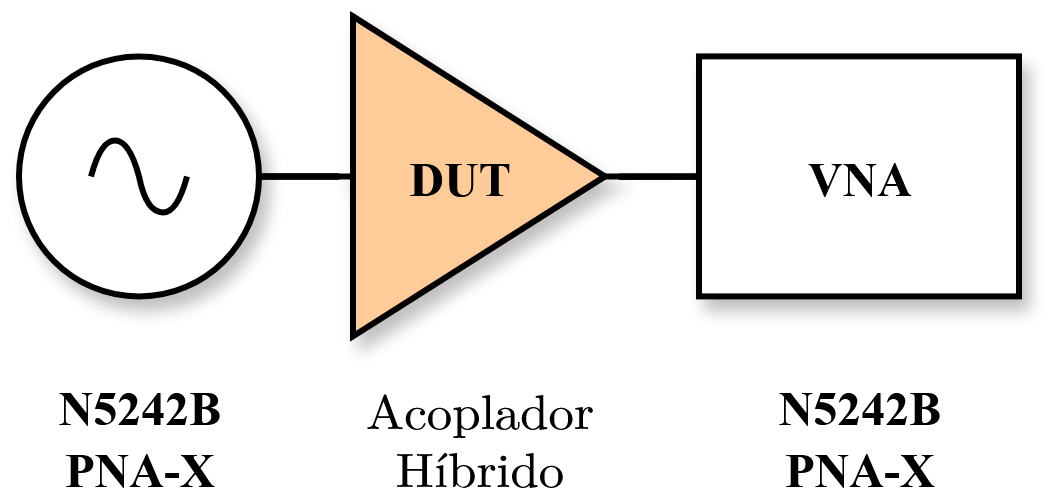
\includegraphics[width=0.5\linewidth]{Figures/07/blocks_coupler.png}
    \caption{Diagrama en bloques del setup de medición de parámetros dispersión del acoplador.}
    \label{fig:setup_medicion_acoplador}
\end{figure}

\subsection{Mediciones del amplificador}
Para validar experimentalmente el diseño propuesto del amplificador, se llevó a cabo un conjunto de mediciones que abarcan el comportamiento de pequeña señal, el desempeño de potencia en gran señal y la caracterización no lineal del dispositivo.

% -----------------------------------------------------------------------------------------------%
\subsubsection{Medición de parámetros dispersión}
Los parámetros de dispersión se midieron con el objetivo de validar el diseño de las redes de adaptación y caracterizar el comportamiento de pequeña señal del amplificador. Se empleó el mismo PNA-X que para las mediciones del acoplador, calibrado mediante el método TOSM con un kit de calibración Keysight 85052B~\cite{calkit}. En el puerto de salida se insertaron en cascada un atenuador de 20\,dB y otro de 10\,dB con el fin de proteger el receptor del VNA frente a los niveles de potencia elevados presentes a la salida del amplificador. En consecuencia, únicamente se reportan los parámetros $S_{21}$ y $S_{11}$, dado que la presencia del atenuador en el puerto de salida impide una medición confiable de los parámetros que involucran la reflexión hacia dicho puerto. El valor medido de $S_{21}$ fue corregido sumando el valor nominal del atenuador.

\begin{figure}[H]
    \centering
    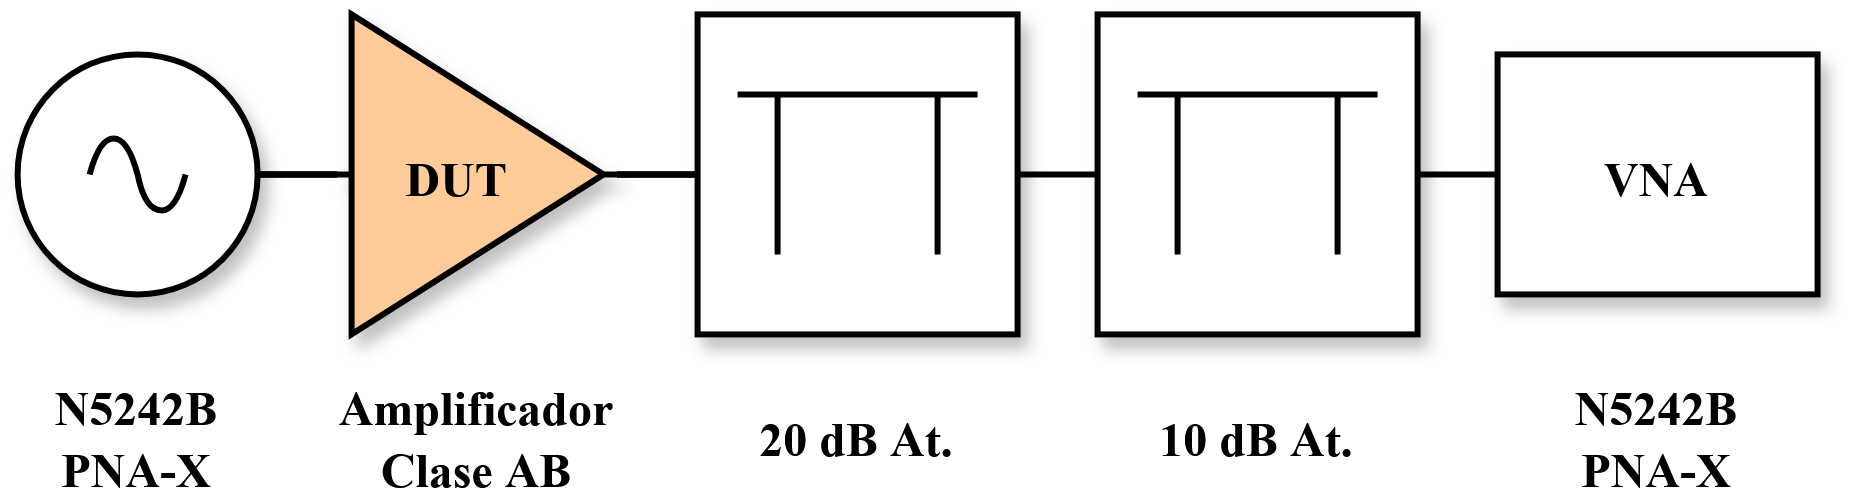
\includegraphics[width=0.8\linewidth]{Figures/07/blocks_sparams.png}
    \caption{Diagrama en bloques del setup de medición de parámetros dispersión del amplificador.}
    \label{fig:setup_medicion_sparam_amp}
\end{figure}

% -----------------------------------------------------------------------------------------------%
\subsubsection{Medición de potencia de salida}
Se realizó una medición de potencia de salida con el fin de caracterizar el comportamiento de gran señal del amplificador. Dado que el dispositivo bajo prueba requiere niveles de excitación superiores a la potencia de salida que el VNA es capaz de entregar, se insertó un amplificador driver Mini-Circuits ZX60-83LN12+~\cite{preamp} entre la fuente de señal del Keysight N5242B y el amplificador de potencia bajo prueba. La potencia de salida se midió con un sensor de potencia Keysight U8485A~\cite{powersensor}, precedido por un atenuador de 20\,dB y un atenuador de 10\,dB. La potencia de entrada se barrió en pasos de 2,5\,dBm a la frecuencia nominal de operación de 2,2\,GHz. A partir de los valores de potencia de entrada y de salida obtenidos mediante este barrido, junto con la medición de la corriente de polarización de drain, se determinaron la ganancia, el punto de compresión de 1\,dB, la potencia de saturación (Psat), la eficiencia de drain y la eficiencia de agregado de potencia (PAE) del amplificador.

\begin{figure}[H]
    \centering
    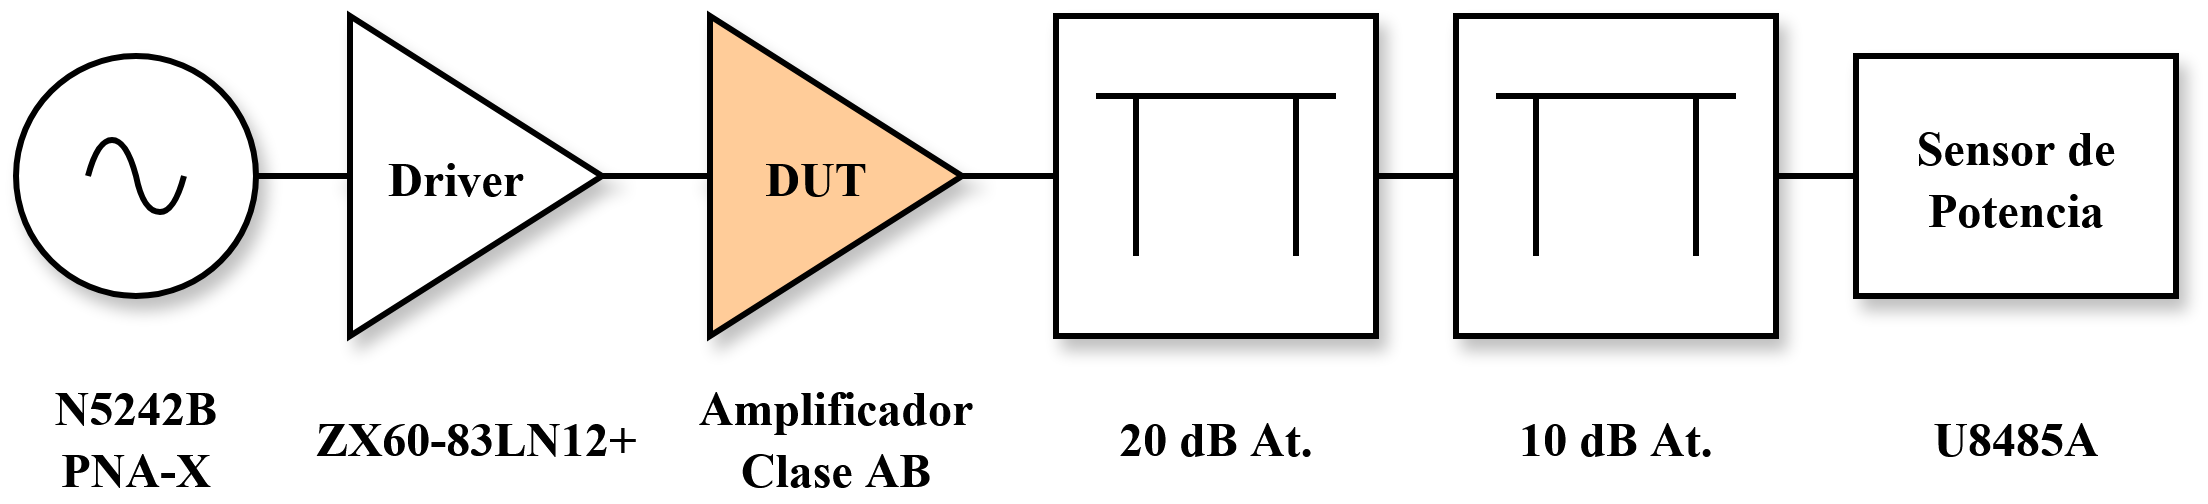
\includegraphics[width=\linewidth]{Figures/07/blocks_p1db.png}
    \caption{Diagrama en bloques del setup de medición de potencia de salida del amplificador.}
    \label{fig:setup_medicion_pout}
\end{figure}

Dado que el amplificador driver ingresa en compresión dentro del rango de medición, el punto de compresión de 1\,dB del dispositivo bajo prueba no puede obtenerse de forma directa a partir de la curva de potencia de salida medida. Por este motivo, se aplicó la expresión de compresión en cascada de la ecuación~\eqref{eq:p1db_cascada}, que refiere la compresión de cada etapa a la entrada del sistema y combina sus contribuciones ponderadas inversamente por la ganancia de las etapas precedentes

\begin{equation}
    \frac{1}{P_{1dB\,sys}} = \frac{1}{G_2 \cdots G_N \, P_{1dB,1}} + \frac{1}{G_3 \cdots G_N \, P_{1dB,2}} + \cdots + \frac{1}{P_{1dB,N}}
    \label{eq:p1db_cascada}
\end{equation}

% -----------------------------------------------------------------------------------------------%
\subsubsection{Medición de distorsión armónica}
Debido a la no linealidad intrínseca de todo dispositivo activo, sumada a la clase de operación en la que se polariza el amplificador, las etapas de potencia generan distorsión armónica que degrada la pureza espectral de la señal y puede provocar interferencia fuera de banda. Para caracterizar este comportamiento, se midieron el segundo y el tercer armónico utilizando un generador de señal Siglent SSG3032X-IQE~\cite{rfgen} como fuente de excitación de onda continua a 2,2\,GHz y un analizador de espectro Keysight N9322C~\cite{spectrumanalyzer} a la salida. Se colocó un atenuador de 20\,dB en la entrada del analizador con fines de protección. La potencia de entrada se barrió desde 0\,dBm hasta 20\,dBm en pasos de 5\,dBm.

\begin{figure}[H]
    \centering
    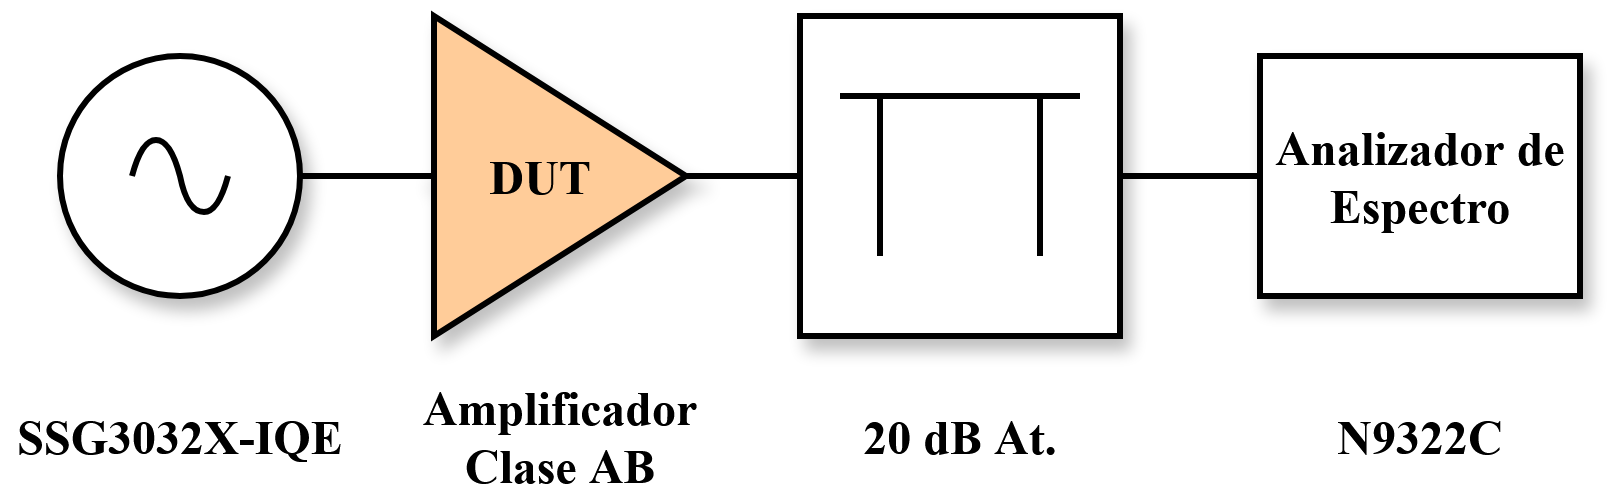
\includegraphics[width=0.7\linewidth]{Figures/07/blocks_harmonic_balance.png}
    \caption{Diagrama en bloques del setup de medición de distorsión armónica del amplificador.}
    \label{fig:setup_medicion_armonicos}
\end{figure}

% -----------------------------------------------------------------------------------------------%
\subsubsection{Medición de OIP3}
Siguiendo el principio de la prueba de dos tonos descripta en la Sección~\ref{sec:dos_tonos}, el punto de intercepción de tercer orden a la salida (OIP3) se obtuvo mediante la aplicación de software ``IMD Sweep'' (S93087B IMD) del VNA Keysight N5242B PNA-X. De forma análoga a la medición de potencia de salida, se incorporó el amplificador driver Mini-Circuits ZX60-83LN12+ entre la fuente de señal del VNA y el dispositivo bajo prueba, con el fin de capturar adecuadamente los efectos de gran señal. Asimismo, se agregaron dos atenuadores de 20\,dB y 10\,dB a la salida del dispositivo bajo prueba para proteger los puertos del VNA. La separación de frecuencia entre los dos tonos se fijó en 10\,MHz, con una potencia de cada tono de $P_{in}=-5\,\text{dBm}$.

\begin{figure}[H]
    \centering
    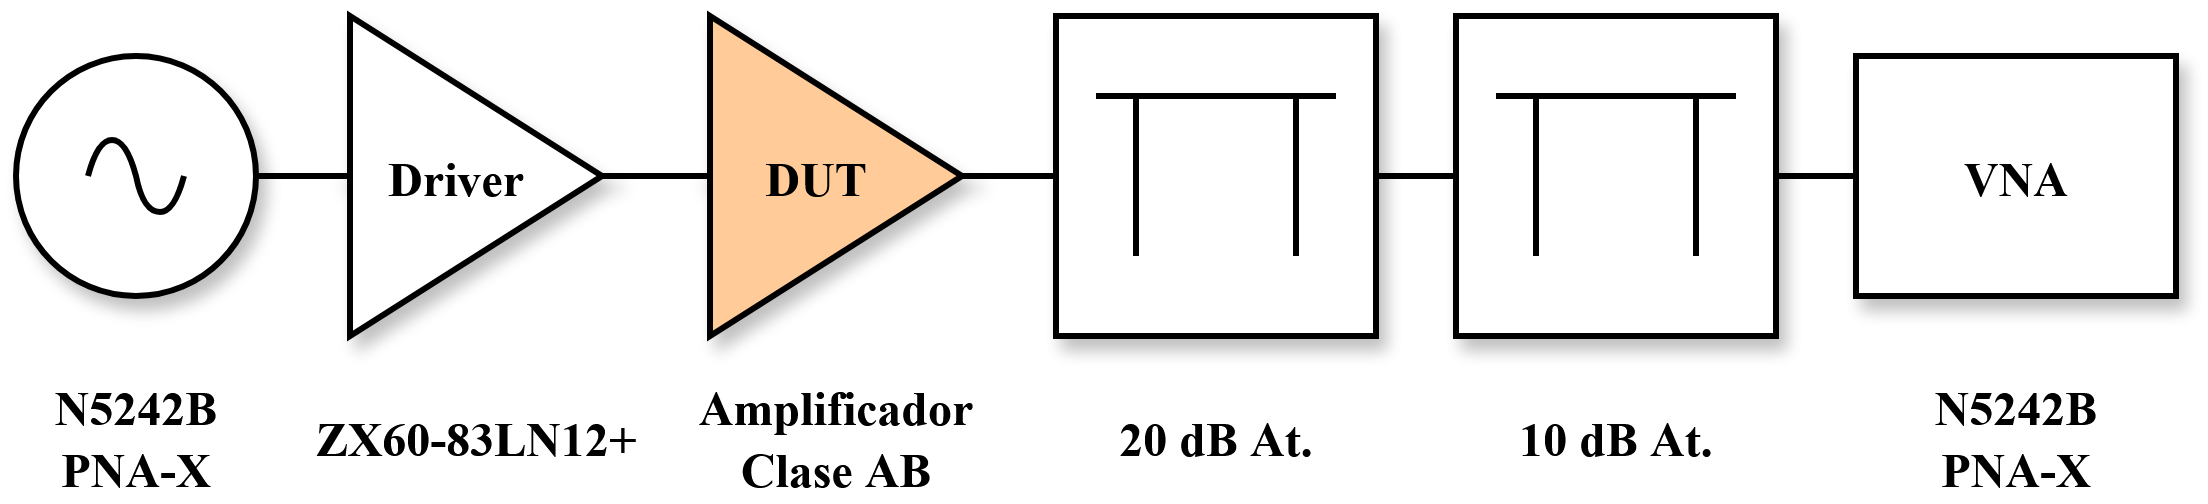
\includegraphics[width=\linewidth]{Figures/07/blocks_oip3.png}
    \caption{Diagrama en bloques del setup de medición de OIP3 del amplificador.}
    \label{fig:setup_medicion_oip3}
\end{figure}
\section{Diseño del acoplador híbrido en cuadratura} \label{sec:diseno_acoplador}
A partir del marco teórico desarrollado en el Capítulo~\ref{cp:introduction}, se abordó el diseño físico del acoplador híbrido en cuadratura mediante la topología de línea ramificada, con el objetivo de emplearlo como primera etapa hacia una arquitectura Doherty. El diseño se planteó en dos versiones sucesivas, denominadas a lo largo de esta sección acoplador v1 y acoplador v2, cuya evolución respondió a hallazgos obtenidos durante la etapa de verificación electromagnética del diseño, descriptos más adelante.

\subsection{Restricción dimensional y topología propuesta}
El híbrido de línea ramificada convencional, tal como se presentó en la Figura~\ref{fig:branch_line_geometry}, se compone de cuatro tramos de línea de transmisión de longitud $\lambda/4$ dispuestos en forma rectangular. Esta longitud eléctrica, que resulta despreciable frente a las dimensiones de un circuito a frecuencias de microondas más elevadas, representa una restricción dimensional significativa en la banda S y en particular para una plataforma CubeSat, donde el área de placa disponible se encuentra fuertemente acotada por el formato normalizado de la plataforma.

% TODO: verificar y referenciar la ecuación de dimensionamiento inicial una vez confirmada
A modo de ejemplo, el dimensionamiento analítico inicial de los tramos de línea que componen el acoplador, obtenido a partir de la síntesis de líneas de transmisión en microstrip sobre el sustrato empleado (permitividad relativa efectiva $\varepsilon_r = 4{,}4$ y altura $h = 0{,}2104$~mm, correspondientes a la capa superior del \textit{stackup} de la Tabla~\ref{tab:pcb_stackup}), arroja longitudes de $\lambda_g/4 \approx 18{,}7$~mm para los tramos en derivación de impedancia $Z_o = 50\,\Omega$ y de $\lambda_g/4 \approx 18{,}3$~mm para los tramos serie de impedancia $Z_o/\sqrt{2} \approx 35{,}36\,\Omega$. Estas dimensiones, dispuestas en la geometría rectangular convencional del híbrido de línea ramificada, resultan en un acoplador de aproximadamente $37 \times 37$~mm, un área que excede ampliamente la disponible en una plataforma CubeSat de formato 1U o 2U una vez descontado el espacio requerido por el resto de la carga útil y los subsistemas de la plataforma.

Con el objetivo de reducir el área ocupada por el acoplador, se optó por una topología de línea ramificada plegada, en la cual cada uno de los cuatro tramos de línea se dobla sobre sí mismo mediante quiebres de 90° distribuidos a lo largo de su longitud, en lugar de disponerse como un tramo recto único. Esta decisión de diseño constituyó uno de los resultados centrales perseguidos en el desarrollo del acoplador, dado que permitió compatibilizar la longitud eléctrica requerida por la teoría de línea ramificada con las restricciones dimensionales impuestas por la plataforma.

Una primera versión de esta topología plegada empleó quiebres con curvatura redondeada. Por recomendación del Ing.~Matías Hampel, dichas curvas se reemplazaron por quiebres rectos, implementados en ADS mediante el componente \texttt{MSABND} (\textit{microstrip bend}), dado que este tipo de geometría facilita el trazado posterior del layout de PCB y reduce la incertidumbre asociada al modelado electromagnético del quiebre. Se evaluaron ángulos de quiebre entre 45° y 90°, seleccionándose finalmente un ángulo de $67{,}5$° por ser el que arrojó el mejor desempeño simulado en términos de adaptación de impedancia y equilibrio entre los puertos de salida.

% TODO: insertar figura con la topología plegada final (esquemático o layout con cotas)
\begin{figure}[H]
    \centering
    % \includegraphics[width=0.8\linewidth]{Figures/acoplador_topologia_plegada.png}
    \caption{Topología plegada propuesta para el acoplador de línea ramificada, con quiebres de 67,5° implementados mediante el componente MSABND.}
    \label{fig:acoplador_topologia_plegada}
\end{figure}

\subsection{Objetivos de diseño}
Los objetivos de diseño del acoplador se establecieron a partir del comportamiento ideal de un híbrido en cuadratura, descripto en la matriz de dispersión de la ecuación~\eqref{eq:quadrature_scattering}. La Tabla~\ref{tab:objetivos_acoplador} resume dichos objetivos.

\begin{table}[H]
    \centering
    \caption{Especificaciones objetivo del acoplador híbrido en cuadratura.}
    \label{tab:objetivos_acoplador}
    \begin{tabular}{lcc}
        \hline\hline
        \textbf{Parámetro}                               & \textbf{Valor Objetivo} & \textbf{Unidad} \\
        \hline
        Frecuencia central ($f_0$)                       & 2,2                     & GHz             \\
        BW ($S_{11} < -10$ dB)                           & XX                      & MHz             \\
        Coeficiente de acoplamiento ($S_{21}$, $S_{31}$) & $-3$                    & dB              \\
        Desbalance de amplitud entre puertos 2 y 3       & XX                      & dB              \\
        Desfasaje entre puertos 2 y 3                    & 90                      & °               \\
        Aislación ($S_{41}$)                             & mínima posible          & dB              \\
        \hline\hline
    \end{tabular}
\end{table}

De acuerdo con estos objetivos, el diseño buscó aproximar en la mayor medida posible el comportamiento del acoplador real al del híbrido ideal caracterizado en la Sección~\ref{cp:introduction}, es decir, entregar una fracción idéntica de la potencia de entrada a los puertos 2 y 3, con un desfasaje de 90° entre ambas señales, mientras se minimiza la potencia acoplada al puerto 4.

\subsection{Diseño esquemático y simulación en ADS}
Siguiendo la metodología de diseño y simulación descripta en la Sección~\ref{sec:metodologia_diseno_sim}, el diseño esquemático del acoplador se llevó a cabo en ADS, empleando líneas de transmisión microstrip sobre el sustrato correspondiente al \textit{stackup} de la Tabla~\ref{tab:pcb_stackup} y quiebres de 67,5° modelados mediante el componente \texttt{MSABND} en cada uno de los cuatro tramos plegados. Sobre este esquemático se ejecutaron rutinas de optimización numérica para ajustar el ancho y el largo de cada tramo de línea, partiendo de las dimensiones analíticas obtenidas en la subsección anterior, hasta alcanzar los objetivos de diseño de la Tabla~\ref{tab:objetivos_acoplador} en la frecuencia de operación.

% TODO: insertar figura del esquemático ADS
\begin{figure}[H]
    \centering
    % \includegraphics[width=\linewidth]{Figures/acoplador_esquematico_ads.png}
    \caption{Esquemático del acoplador híbrido en ADS.}
    \label{fig:acoplador_esquematico_ads}
\end{figure}

% TODO: insertar figura de resultados de parámetros S simulados en ADS (esquemático)
\begin{figure}[H]
    \centering
    % \includegraphics[width=\linewidth]{Figures/acoplador_resultados_ads.png}
    \caption{Parámetros de dispersión simulados del acoplador a nivel esquemático en ADS, luego de la optimización.}
    \label{fig:acoplador_resultados_ads}
\end{figure}

Los resultados obtenidos a nivel de esquemático se consideraron satisfactorios respecto de los objetivos de diseño planteados, lo que habilitó el avance hacia la etapa de diseño físico del circuito impreso.

\subsection{Diseño de PCB}
Siguiendo la metodología de diseño de PCB descripta en la Sección~\ref{sec:metodologia_pcb}, el layout del acoplador se exportó desde el entorno de layout de ADS en formato DXF. Dado que la importación directa de este archivo en Altium Designer presentó inconsistencias en algunos segmentos del dibujo, que desaparecían durante el proceso de importación, se adoptó una ruta de conversión alternativa consistente en importar el archivo DXF a Ansys CST, reexportarlo desde dicho entorno y finalmente importarlo a Altium, lo que resolvió el inconveniente.

Sobre el layout resultante se aplicaron, además de los criterios generales descriptos en la Sección~\ref{sec:metodologia_pcb}, las siguientes consideraciones específicas del diseño del acoplador:

\begin{itemize}
    \item Los \textit{pads} de masa de los conectores SMA se ubicaron lo más próximos posible al borde de la placa, con el objetivo de minimizar la longitud de la transición entre el conector y la línea microstrip.
    \item Se aplicó un mallado de vías (\textit{via stitching}) sobre el plano de masa de la capa superior, en el contorno de la geometría del acoplador, con el fin de reforzar la continuidad de la referencia de masa en la vecindad de las líneas plegadas.
    \item Las vías se configuraron con tapado de máscara de soldadura (\textit{tented vias}), con el objetivo de evitar dejar cobre expuesto en los puntos de conexión a masa.
    \item Dado que la simulación electromagnética del acoplador asumió que las líneas microstrip se encontraban expuestas al aire, sin cobertura dieléctrica adicional, se removió la máscara de soldadura sobre la totalidad del trazado del acoplador, con el fin de que la placa fabricada se correspondiera con la condición asumida en la simulación.
\end{itemize}

% TODO: insertar figura del layout final de PCB (v1)
\begin{figure}[H]
    \centering
    % \includegraphics[width=\linewidth]{Figures/acoplador_pcb_v1.png}
    \caption{Layout de PCB de la primera versión del acoplador híbrido.}
    \label{fig:acoplador_pcb_v1}
\end{figure}

\subsection{Verificación electromagnética y segunda iteración de diseño}
Con el objetivo de validar el comportamiento del acoplador considerando los efectos electromagnéticos no capturados por el modelo de líneas de transmisión analíticas empleado en ADS, se realizó una simulación de onda completa del layout de PCB en Ansys HFSS. Esta verificación reveló que la frecuencia central efectiva del acoplador se encontraba corrida hacia abajo de manera considerable respecto de la frecuencia de diseño de 2,2~GHz, ubicándose entre 1,8~GHz y 1,9~GHz. No obstante, los valores de desfasaje y de atenuación obtenidos en dicha frecuencia central corrida resultaron similares a los previstos por la simulación en ADS, lo que indicó que el corrimiento afectaba principalmente a la frecuencia de operación del circuito y no a su comportamiento cualitativo como híbrido en cuadratura.

Al analizar el origen de esta discrepancia, se determinó que el esquemático de ADS empleado para el diseño y la optimización no incluía la contribución de la transición entre la línea microstrip y el conector SMA, cuyo pad de conexión introduce una longitud de línea adicional no considerada en el dimensionamiento original. Para verificar esta hipótesis, se agregó en ADS, a la entrada de cada uno de los cuatro puertos del acoplador, un tramo de línea adicional de $3{,}6 \times 1{,}27$~mm² destinado a modelar dicho \textit{pad} de conexión. Al incorporar estos tramos, el corrimiento de la frecuencia central observado en la simulación esquemática reprodujo el mismo comportamiento identificado en la simulación electromagnética del layout, confirmando la causa del corrimiento.

A partir de este hallazgo, se definió una segunda versión del acoplador (acoplador v2), en la cual se repitió la rutina de optimización sobre el esquemático de ADS incluyendo los tramos adicionales que modelan la conexión con el SMA, con el objetivo de compensar el corrimiento de frecuencia identificado. El layout de PCB correspondiente a esta segunda versión se rediseñó siguiendo las mismas consideraciones descriptas en la subsección anterior.

% TODO: insertar figura de resultados ADS v2 (con pad SMA modelado)
\begin{figure}[H]
    \centering
    % \includegraphics[width=\linewidth]{Figures/acoplador_resultados_ads_v2.png}
    \caption{Parámetros de dispersión simulados del acoplador v2, incluyendo el modelado del pad de conexión SMA, luego de la reoptimización.}
    \label{fig:acoplador_resultados_ads_v2}
\end{figure}

% TODO: insertar figura del layout final de PCB (v2)
\begin{figure}[H]
    \centering
    % \includegraphics[width=\linewidth]{Figures/acoplador_pcb_v2.png}
    \caption{Layout de PCB de la segunda versión del acoplador híbrido.}
    \label{fig:acoplador_pcb_v2}
\end{figure}

La medición de parámetros de dispersión del prototipo fabricado, empleada para validar experimentalmente este diseño, se realizó siguiendo la metodología descripta en la Sección~\ref{sec:metodologia_medicion}, y sus resultados se presentan en el Capítulo~\ref{sec:resultados}.
%\section{Diseño del amplificador de potencia} \label{sec:diseno_amplificador}
El amplificador de potencia desarrollado en este trabajo consistió en una topología monoetapa, basada en el transistor GaN HEMT CGH40006S, polarizado en Clase AB y destinado a operar en banda S sobre la frecuencia de portadora de 2,2\,GHz. La elección de una topología de etapa única, en contraposición a una cadena de amplificación multietapa, se fundamentó en que la ganancia del dispositivo seleccionado resulta suficiente para alcanzar la potencia de salida objetivo a partir de un nivel de excitación moderado, evitando así la complejidad adicional, el consumo de área de placa y los riesgos de estabilidad asociados al acoplamiento entre etapas sucesivas, lo cual reduce el número de redes de adaptación de impedancia y de puntos de polarización independientes que deben diseñarse, simularse y ajustarse experimentalmente.

Esta cadena de decisiones responde directamente a las restricciones impuestas por la plataforma CubeSat. La elección del GaN como tecnología semiconductora, fundamentada en la Sección~\ref{sec:gan_hemt} a partir de su elevada densidad de potencia y su figura de mérito de Johnson superior a la del silicio y el GaAs, permite alcanzar la potencia de salida requerida con un dispositivo de área reducida, minimizando la masa del disipador térmico necesario. La operación en Clase AB, justificada a partir del compromiso entre linealidad y eficiencia se complementa con la selección puntual del CGH40006S, cuya tensión de alimentación nominal de drain (28~V) resulta compatible con los niveles de tensión disponibles en el bus de potencia de una plataforma nanosatelital, evitando una etapa de conversión de tensión adicional dedicada al subsistema de RF. El consumo de potencia continua debe contemplarse dentro del presupuesto energético total disponible para la plataforma, el cual se encuentra acotado por la capacidad de generación fotovoltaica y de almacenamiento del sistema de potencia del CubeSat.

El desarrollo completo del amplificador, desde la etapa de diseño asistido por simulación hasta la fabricación y caracterización experimental del prototipo, se describe en las subsecciones siguientes, concluyendo con el análisis de radioenlace realizado a partir de la potencia de salida efectivamente alcanzada por el diseño desarrollado.

% -----------------------------------------------------------------------------------------------%
\subsection{Objetivos de diseño}
Los objetivos de diseño del amplificador coinciden con los requisitos mandatorios establecidos en el Cuadro~\ref{tab:requisitos_clasificados} del Capítulo~\ref{sec:anteproyecto}, previo a la redefinición de alcance del proyecto descripta en el Capítulo~\ref{sec:alcance}, dado que dicha redefinición no modificó las especificaciones eléctricas objetivo del amplificador. El Cuadro~\ref{tab:objetivos_diseno} repite dichos valores por comodidad, junto con el factor de estabilidad, no incluido originalmente en la clasificación de requisitos.

\begin{table}[H]
    \centering
    \caption{Especificaciones objetivo del amplificador de potencia.}
    \label{tab:objetivos_diseno}
    \begin{tabular}{lcc}
        \hline\hline
        \textbf{Parámetro}                   & \textbf{Valor Objetivo} & \textbf{Unidad} \\
        \hline
        Frecuencia central ($f_0$)           & 2,2                     & GHz             \\
        BW ($S_{11} < -10$ dB)               & 35                      & MHz             \\
        $P_{out}$                            & $\ge$ 1                 & W               \\
        PAE                                  & $\ge$ 35                & \%              \\
        OIP3                                 & $\ge$ 35                & dBm             \\
        Factor de estabilidad ($\mu$)        & $> 1$ (incond.)         & ---             \\
        \hline\hline
    \end{tabular}
\end{table}

% -----------------------------------------------------------------------------------------------%
\subsection{Transistor seleccionado y topología propuesta}
El transistor seleccionado para el diseño del amplificador de potencia fue el CGH40006S, un GaN HEMT discreto fabricado originalmente por Cree y comercializado actualmente por MACOM, encapsulado en formato de montaje superficial. La selección de este dispositivo se fundamentó en los siguientes criterios:

\begin{enumerate}
    \item \textbf{Especificaciones eléctricas adecuadas a la aplicación:} el dispositivo entrega una potencia de salida en el punto de compresión de 1~dB de aproximadamente 37,5~dBm a 2~GHz, con una ganancia de pequeña señal del orden de 20~dB y una PAE cercana al 60\,\%, valores que exceden ampliamente el requisito de 1~W (30~dBm) de salida establecido para la misión, lo que otorga margen de diseño respecto del punto de compresión \cite{Macom}.

    \item \textbf{Disponibilidad de modelo no lineal del fabricante:} MACOM provee un modelo no lineal del CGH40006S compatible con entornos de simulación de circuitos de microondas, lo que permitió realizar simulaciones de gran señal del amplificador previas a la fabricación del prototipo físico, reduciendo el riesgo de iteraciones costosas en hardware. Otros fabricantes de transistores GaN HEMT discretos no facilitan de manera igualmente sencilla el acceso a estos modelos no lineales, condición que en la práctica acotó considerablemente el catálogo de dispositivos considerado viable para el proyecto, y motivó priorizar la selección de un transistor de MACOM.
    
    \item \textbf{Eficiencia en el punto de operación:} para obtener la máxima eficiencia posible de un dispositivo, resulta necesario operarlo en una región de trabajo próxima a su punto de máxima potencia. Dado que el CGH40006S está especificado para una potencia de saturación de 6~W, operarlo en torno a los 2~W requeridos por la aplicación permite alcanzar una eficiencia sustancialmente mayor que la que se obtendría empleando un transistor de mayor potencia nominal (por ejemplo, uno especificado para 15~W) en ese mismo punto de trabajo, dado que este último operaría muy por debajo de su región de máxima eficiencia.

    \item \textbf{Costo moderado dentro del segmento de GaN HEMT discretos:} al momento de redacción de este trabajo, el costo unitario del dispositivo se ubica en torno a los 75~USD, valor que se considera moderado para el segmento de transistores GaN HEMT discretos orientados a aplicaciones profesionales y aeroespaciales, en contraste con soluciones de mayor integración como los circuitos monolíticos de microondas (MMIC), cuyo costo y plazo de adquisición suelen ser sustancialmente mayores.

\end{enumerate}

La Figura~\ref{fig:diagrama_bloques} presenta el diagrama en bloques de la topología propuesta para el amplificador. La señal de entrada de radiofrecuencia ingresa a la red de adaptación de entrada, la cual, además de transformar la impedancia del generador a la impedancia óptima de fuente del transistor, cumple la función de filtro pasaaltos y bloqueo de continua, e incorpora una derivación destinada a la inyección de la polarización de gate, aislada de la señal mediante un inductor actuando de choke de RF. A continuación, la señal atraviesa la red de estabilidad, cuya topología concreta fue objeto de sucesivas revisiones a lo largo del proceso de diseño, con el objetivo de extender el margen de estabilidad del circuito hacia frecuencias por debajo de la banda de operación sin comprometer significativamente la ganancia. El transistor CGH40006S amplifica la señal en Clase AB, entregándola a la red de adaptación de salida, la cual transforma la impedancia óptima de carga del transistor a la impedancia de $50\,\Omega$ del sistema, incorpora stubs en cortocircuito para suprimir el contenido armónico no deseado, capacitores de bloqueo de continua, y una derivación para la inyección de la polarización de drain, aislada de la señal de RF mediante una línea de transmisión de $\lambda/4$. Las tensiones y corrientes de polarización nominales adoptadas para el circuito son $V_{GG}=-2,6$~V e $I_G=7$~mA en el gate, y $V_{DD}=28$~V e $I_D=100$~mA en el drain.

\begin{figure}[H]
    \centering
    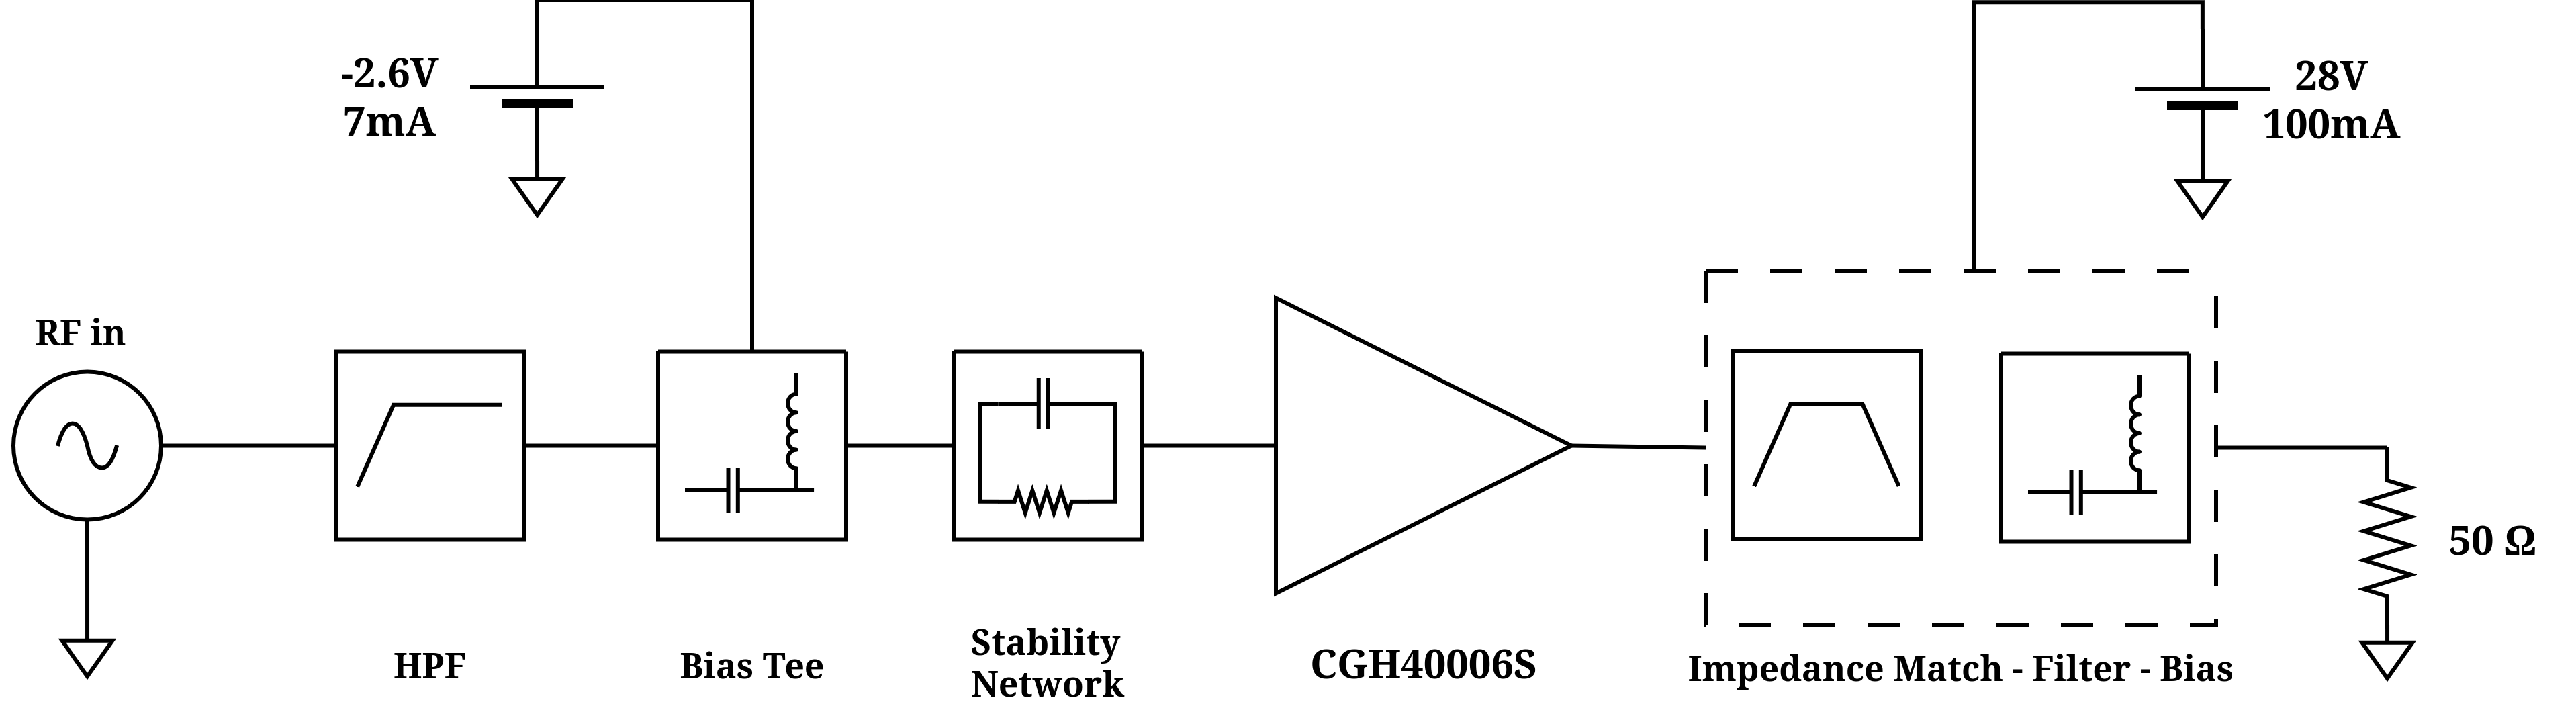
\includegraphics[width=\linewidth]{Figures/07/pa_block_diagram.png}
    \caption{Diagrama en bloques de la topología propuesta para el amplificador de potencia.}
    \label{fig:diagrama_bloques}
\end{figure}

% -----------------------------------------------------------------------------------------------%
\subsection{Diseño esquemático y simulación en ADS}
El proceso de diseño se desarrolló de manera iterativa, comenzando por el análisis de estabilidad del transistor, continuando con la determinación de las impedancias óptimas de carga y de entrada mediante load-pull, y finalizando con el diseño de las redes de adaptación físicas y su verificación con componentes reales.

\textbf{Red de estabilidad.} El primer paso del diseño consistió en evaluar la estabilidad del transistor desnudo, es decir, sin ninguna red adicional de estabilización, en función del punto de polarización. Para ello se armó en ADS el esquemático de la Figura~\ref{fig:pa_ads_stb_bare}, en el cual se polarizó al transistor y se realizó un barrido de la tensión de gate entre -3,5~V y -1,5~V, con $V_{DS}=28$~V fijo, evaluando el factor de estabilidad de Rollett ($K$) entre 0,1 y 6~GHz. Previamente, se validó el modelo del transistor contra la información de la nota de aplicación del fabricante, reproduciendo las curvas características $I_{DS}$-$V_{DS}$ y de transconductancia $G_m$ en función de $V_{GS}$.

\begin{figure}[H]
    \centering
    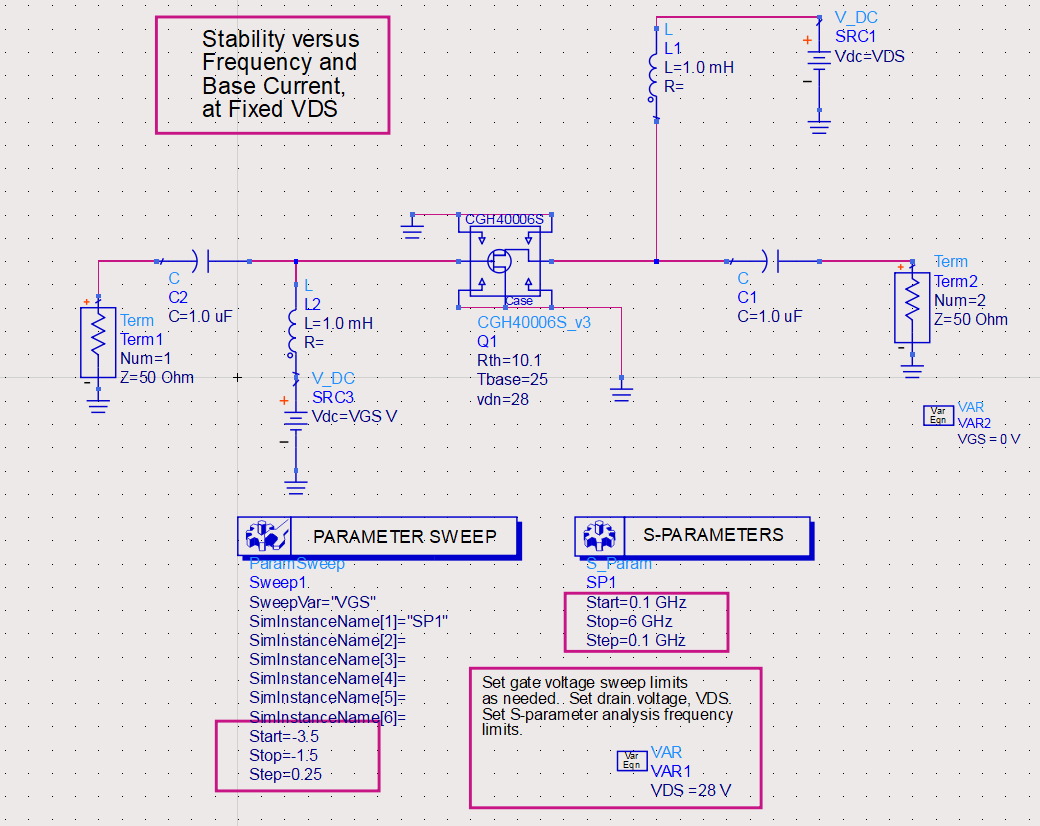
\includegraphics[width=0.7\linewidth]{Figures/07/pa_ads_stb_bare.png}
    \caption{Esquemático empleado para el barrido de estabilidad del transistor en función de la tensión de gate, sin red de estabilidad adicional.}
    \label{fig:pa_ads_stb_bare}
\end{figure}

La Figura~\ref{fig:pa_ads_kfactor_bare} muestra el resultado de este barrido. El caso $V_{GS}=-3,5$~V resulta estable ($K>1$) en toda la banda, pero se trata de un caso trivial, dado que en ese punto el transistor se encuentra en la región de corte y no conduce corriente. Para el resto de los casos, en los que el transistor sí conduce, el factor $K$ mejora a medida que $V_{GS}$ aumenta (se hace menos negativa), estabilizándose a partir de aproximadamente $V_{GS}=-2,5$~V, sin mejoras adicionales significativas por encima de este valor. Aun así, en todos estos casos en los que el transistor conduce, el circuito resulta potencialmente inestable ($K$<1) a bajas frecuencias, lo que evidencia la necesidad de una red de estabilización.

\begin{figure}[H]
    \centering
    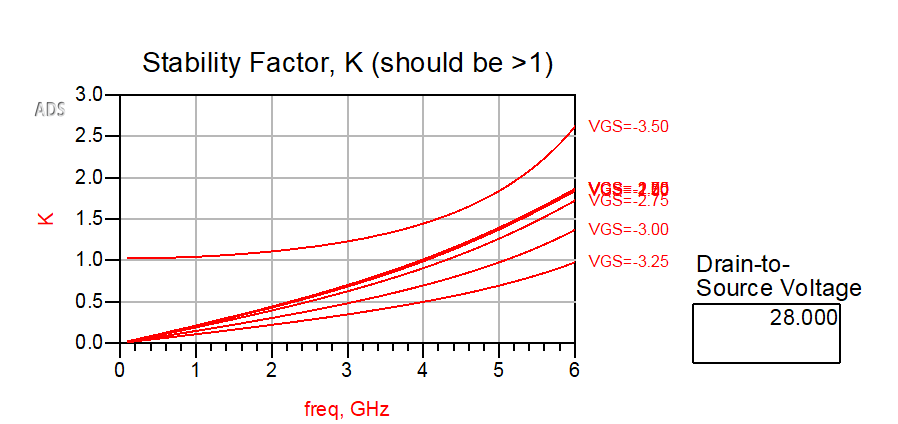
\includegraphics[width=0.8\linewidth]{Figures/07/pa_ads_kfactor_bare.png}
    \caption{Factor de estabilidad de Rollett ($K$) en función de la frecuencia, para distintos valores de $V_{GS}$, sin red de estabilidad adicional.}
    \label{fig:pa_ads_kfactor_bare}
\end{figure}

Se evaluó en primer lugar la incorporación de una resistencia serie de bajo valor en el gate (5, 10 y 50~$\Omega$) como única medida de estabilización, la cual no resultó suficiente para lograr estabilidad incondicional en ninguno de los tres casos. Siguiendo el criterio de diseño de la nota de aplicación del fabricante \cite{macom2023an}, reproducido en la Figura~\ref{fig:pa_an_stb_net}, se incorporó adicionalmente una red de realimentación resistivo-capacitiva entre drain y gate ($R=432\,\Omega$, $C=82$~pF), en conjunto con la resistencia serie de gate ($R=5\,\Omega$), conformando el esquemático de la Figura~\ref{fig:pa_ads_stb_sch_v1}.

\begin{figure}[H]
    \centering
    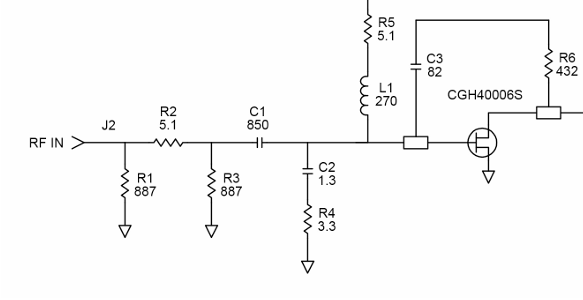
\includegraphics[width=0.8\linewidth]{Figures/07/pa_an_stb_net.png}
    \caption{Red de estabilidad de referencia propuesta en la nota de aplicación del fabricante del transistor \cite{macom2023an}.}
    \label{fig:pa_an_stb_net}
\end{figure}

\begin{figure}[H]
    \centering
    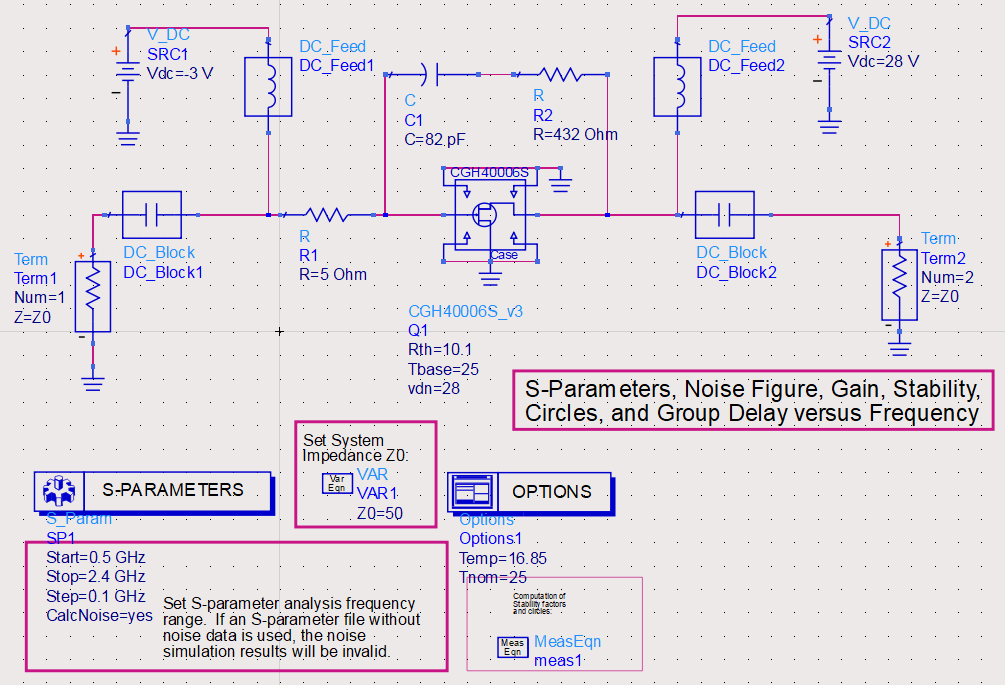
\includegraphics[width=\linewidth]{Figures/07/pa_ads_stb_sch_v1.png}
    \caption{Esquemático de la primera red de estabilidad implementada en ADS, con resistencia serie de gate y realimentación resistivo-capacitiva entre drain y gate.}
    \label{fig:pa_ads_stb_sch_v1}
\end{figure}

Con esta red incorporada, se evaluó la estabilidad incondicional del circuito mediante los factores $\mu_{load}$ y $\mu_{source}$, cuyo resultado se presenta en la Figura~\ref{fig:pa_ads_mu_v1}. Ambos factores resultaron mayores a la unidad en la totalidad de la banda simulada (0 a 6~GHz) y para todos los puntos de polarización evaluados, confirmando la estabilidad incondicional del circuito. Esta conclusión se verificó adicionalmente mediante una simulación de adaptación simultánea, ruido y círculos de estabilidad, cuyo resultado se muestra en la Figura~\ref{fig:pa_ads_stbcircles_v1}: la ausencia de círculos de inestabilidad de carga dentro del diagrama de Smith indica que, para el punto de polarización analizado, el circuito resulta estable frente a cualquier condición de carga posible.

\begin{figure}[H]
    \centering
    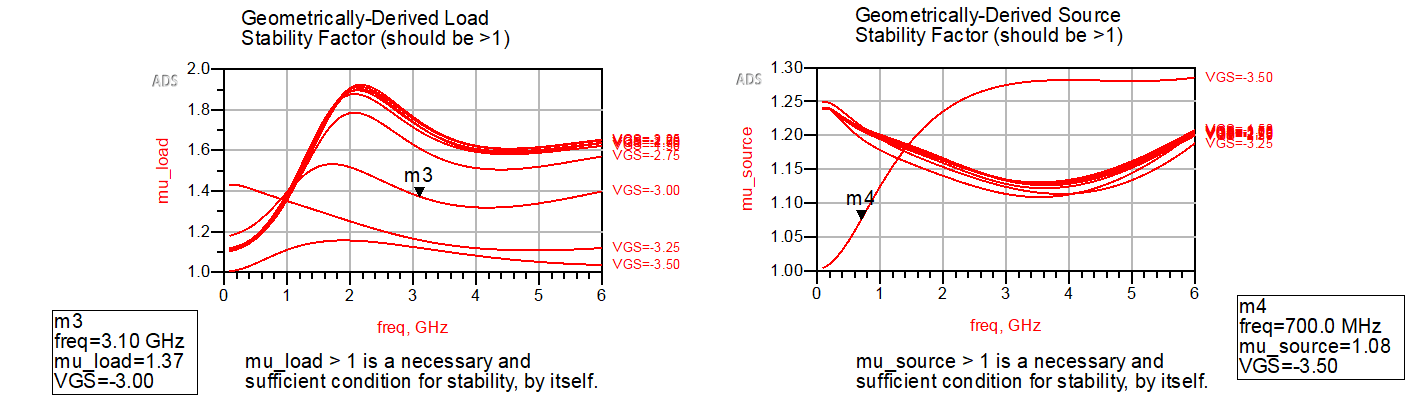
\includegraphics[width=\linewidth]{Figures/07/pa_ads_mu_v1.png}
    \caption{Factores de estabilidad de carga ($\mu_{load}$) y de fuente ($\mu_{source}$) en función de la frecuencia, para la primera red de estabilidad implementada.}
    \label{fig:pa_ads_mu_v1}
\end{figure}

\begin{figure}[H]
    \centering
    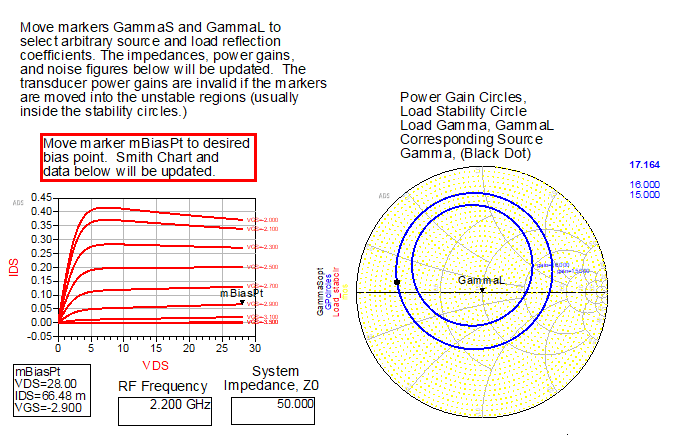
\includegraphics[width=0.7\linewidth]{Figures/07/pa_ads_stbcircles_v1.png}
    \caption{Círculos de ganancia de potencia y de estabilidad de carga en el diagrama de Smith, sin círculos de inestabilidad presentes dentro de la región de interés, confirmando estabilidad incondicional.}
    \label{fig:pa_ads_stbcircles_v1}
\end{figure}

A continuación fue llevada a cabo una simulación de load-pull para determinar las impedancias de carga y de fuente ($\Gamma_L$ y $\Gamma_S$) del transistor. Sin embargo, este análisis no contemplaba la línea de transmisión física necesaria para conectar la resistencia y el capacitor de la red de estabilidad. Al avanzar hacia el diseño físico e incorporar dicha línea, se identificó que esta introducía una fase adicional que volvía inestable al circuito, a pesar de que la red discreta ideal garantizaba estabilidad incondicional. Este hallazgo obligó a rediseñar la red de estabilidad teniendo en cuenta explícitamente el efecto de la línea de transmisión, hasta recuperar la condición de estabilidad incondicional.

Dado que este rediseño modificaba las condiciones de carga y de fuente vistas por el transistor, fue necesario repetir el load-pull para obtener nuevos valores de $\Gamma_L$ y $\Gamma_S$ consistentes con la red de estabilidad ya corregida. Al evaluar esta nueva solución se observó que la resistencia de la red de estabilidad disipaba aproximadamente 1~W, por lo que, en lugar de continuar iterando sobre el mismo criterio, se optó por cambiar la estrategia de diseño, abandonando la búsqueda de estabilidad incondicional en favor de un diseño condicionalmente estable, es decir, estable para el mayor rango posible de condiciones de carga y de fuente, pero no necesariamente para la totalidad del diagrama de Smith. Esta decisión se fundamenta en que garantizar estabilidad incondicional compromete de manera significativa la ganancia, la eficiencia y la potencia de salida del amplificador, mientras que una solución condicionalmente estable, correctamente delimitada, permite recuperar gran parte de estas prestaciones a cambio de restringir el diseño de la red de adaptación a una región acotada del diagrama de Smith.

El nuevo diseño de la red de estabilidad se basó en \cite{bahl2009}, consistiendo esta en un circuito RC paralelo ($R=25~\Omega, C=5~pF$) en el gate del transistor, como se observa en la Figura~\ref{fig:pa_ads_stb_sch_v2}. Ante este nuevo diseño, el análisis de $\mu_{load}$ en función de la frecuencia y del punto de polarización fue repetido, el cual se presenta en la Figura~\ref{fig:pa_ads_mu_v2}. A diferencia del caso incondicionalmente estable de la Figura~\ref{fig:pa_ads_mu_v1}, en este caso $\mu_{load}$ se hace menor a la unidad a partir de aproximadamente 700~MHz para la polarización nominal ($V_{GS}=-3$\,~V), lo cual es esperable y aceptable dado el nuevo criterio de diseño adoptado. Al elevar ligeramente el punto de polarización hacia la región de Clase AB ($V_{GS}=-2,75$\,~V), este cruce se desplaza hasta aproximadamente 500~MHz, lo que evidencia que el punto de polarización constituye una variable de la cual depende el margen de estabilidad.

\begin{figure}[H]
    \centering
    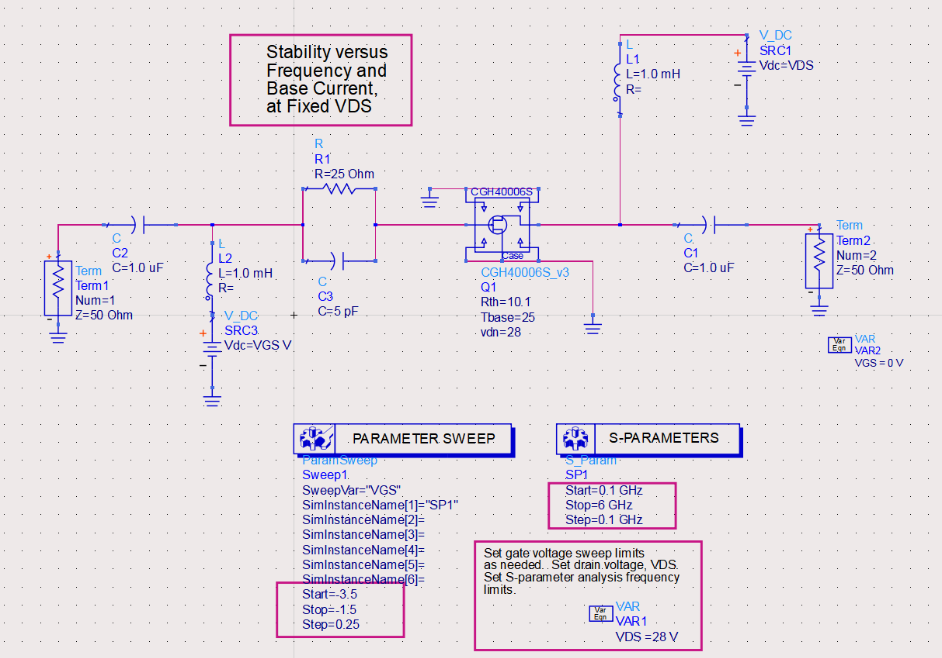
\includegraphics[width=\linewidth]{Figures/07/pa_ads_stb_sch_v2.png}
    \caption{Esquemático de la segunda red de estabilidad implementada en ADS con circuito RC paralelo en serie al gate del transistor.}
    \label{fig:pa_ads_stb_sch_v2}
\end{figure}

\begin{figure}[H]
    \centering
    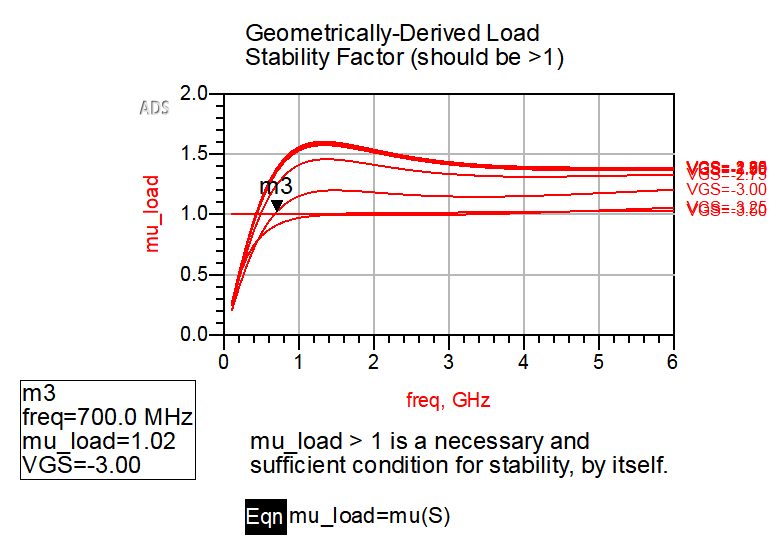
\includegraphics[width=0.8\linewidth]{Figures/07/pa_ads_mu_v2.png}
    \caption{Factor de estabilidad de carga ($\mu_{load}$) en función de la frecuencia, para la red de estabilidad condicionalmente estable, en distintos puntos de polarización de gate.}
    \label{fig:pa_ads_mu_v2}
\end{figure}

A partir de este análisis se identificaron dos frecuencias críticas para el diseño de la red de adaptación. La primera, de 700~MHz, corresponde al punto en el que el circuito comienza a presentar una región de inestabilidad. La segunda, de 350~MHz, se vincula con la longitud de onda guiada de aproximadamente 40~cm, dado que una línea de transmisión deja de comportarse como tal, y pasa a comportarse aproximadamente como un conductor que refleja directamente la impedancia de su terminación, cuando su longitud resulta inferior a $\lambda/10$, es decir, inferior a 4~cm para esta frecuencia. En consecuencia, el objetivo de diseño de la red de adaptación se estableció en presentar la menor desadaptación posible por debajo de 700~MHz, evitando que el coeficiente de reflexión visto por el transistor ingrese en la región delimitada por el círculo de inestabilidad de carga en ese rango.

Los círculos de estabilidad se evaluaron en los puntos críticos de 500~MHz y 300~MHz para la polarización nominal, obteniéndose módulos de coeficiente de reflexión límite de 0,841 y 0,566 respectivamente, por debajo de los cuales el circuito permanece estable frente a cualquier condición de carga. Al repetir este análisis para el punto de polarización de Clase AB ($V_{GS}=-2,8$~V) en 300~MHz, el módulo del coeficiente de reflexión límite se incrementó a 0,684, una mejora relativa de aproximadamente el 20\,\% en el radio de la región de cargas admisibles, confirmando nuevamente el efecto beneficioso de operar levemente por encima de la polarización de Clase B estricta sobre el margen de estabilidad del circuito.

\begin{figure}[H]
    \centering
    \begin{subfigure}{0.48\linewidth}
        \centering
        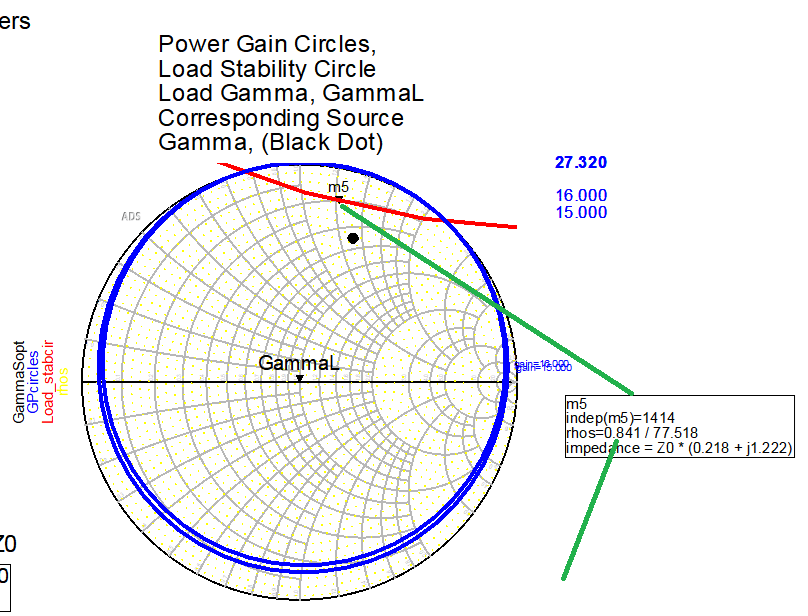
\includegraphics[width=\linewidth]{Figures/07/pa_circulo_500mhz.png}
        \caption{500\,MHz, $V_{GS}=-3$~V ($|\Gamma|=0,841$)}
    \end{subfigure}
    \hfill
    \begin{subfigure}{0.48\linewidth}
        \centering
        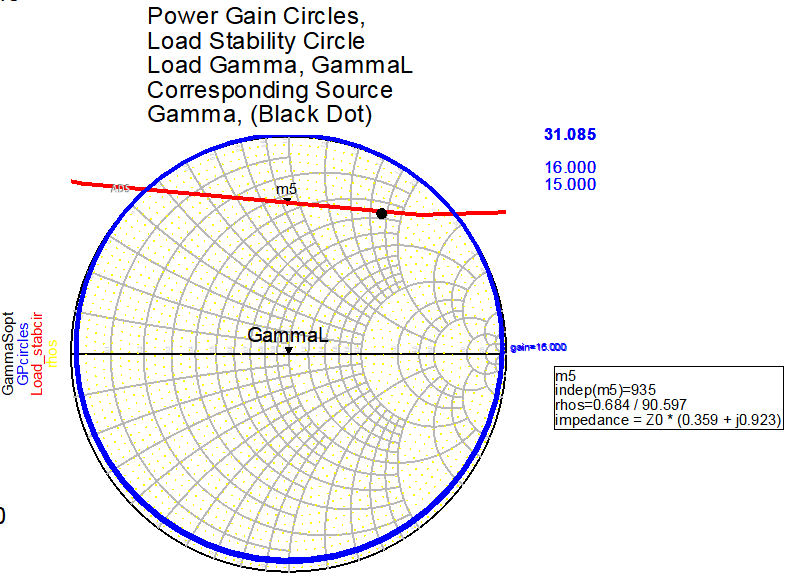
\includegraphics[width=\linewidth]{Figures/07/pa_circulo_300mhz_ab.png}
        \caption{300\,MHz, $V_{GS}=-2,8$~V ($|\Gamma|=0,684$)}
    \end{subfigure}
    \caption{Círculos de estabilidad de carga en el plano de Smith, mostrando el coeficiente de reflexión límite $\rho$ para distintas frecuencias y puntos de polarización.}
    \label{fig:pa_circulos_estabilidad}
\end{figure}

Con el circuito ya prácticamente terminado, y en paralelo con la selección de los componentes reales descripta más adelante, se revisó nuevamente la red de estabilidad, incorporando un nuevo juego de resistencias dispuesto para aumentar simultáneamente la conductancia en paralelo y la resistencia en serie vistas por el transistor. Esta última revisión, presentada en la Figura~\ref{fig:pa_ads_final}, logró nuevamente estabilidad incondicional del circuito, a costa de una pérdida de ganancia que resultó mínima y despreciable frente al beneficio de eliminar el riesgo de oscilaciones no deseadas. En el esquemático puede observarse que las resistencias R3 y R5 incorporan cada una un inductor en serie (L8 y L7 respectivamente), los cuales no forman parte del diseño original de la red sino que modelan la inductancia parásita propia de las resistencias reales seleccionadas, cuyo efecto sobre el desempeño del circuito se analiza en la Sección~\ref{sec:resultados}.

\begin{figure}[H]
    \centering
    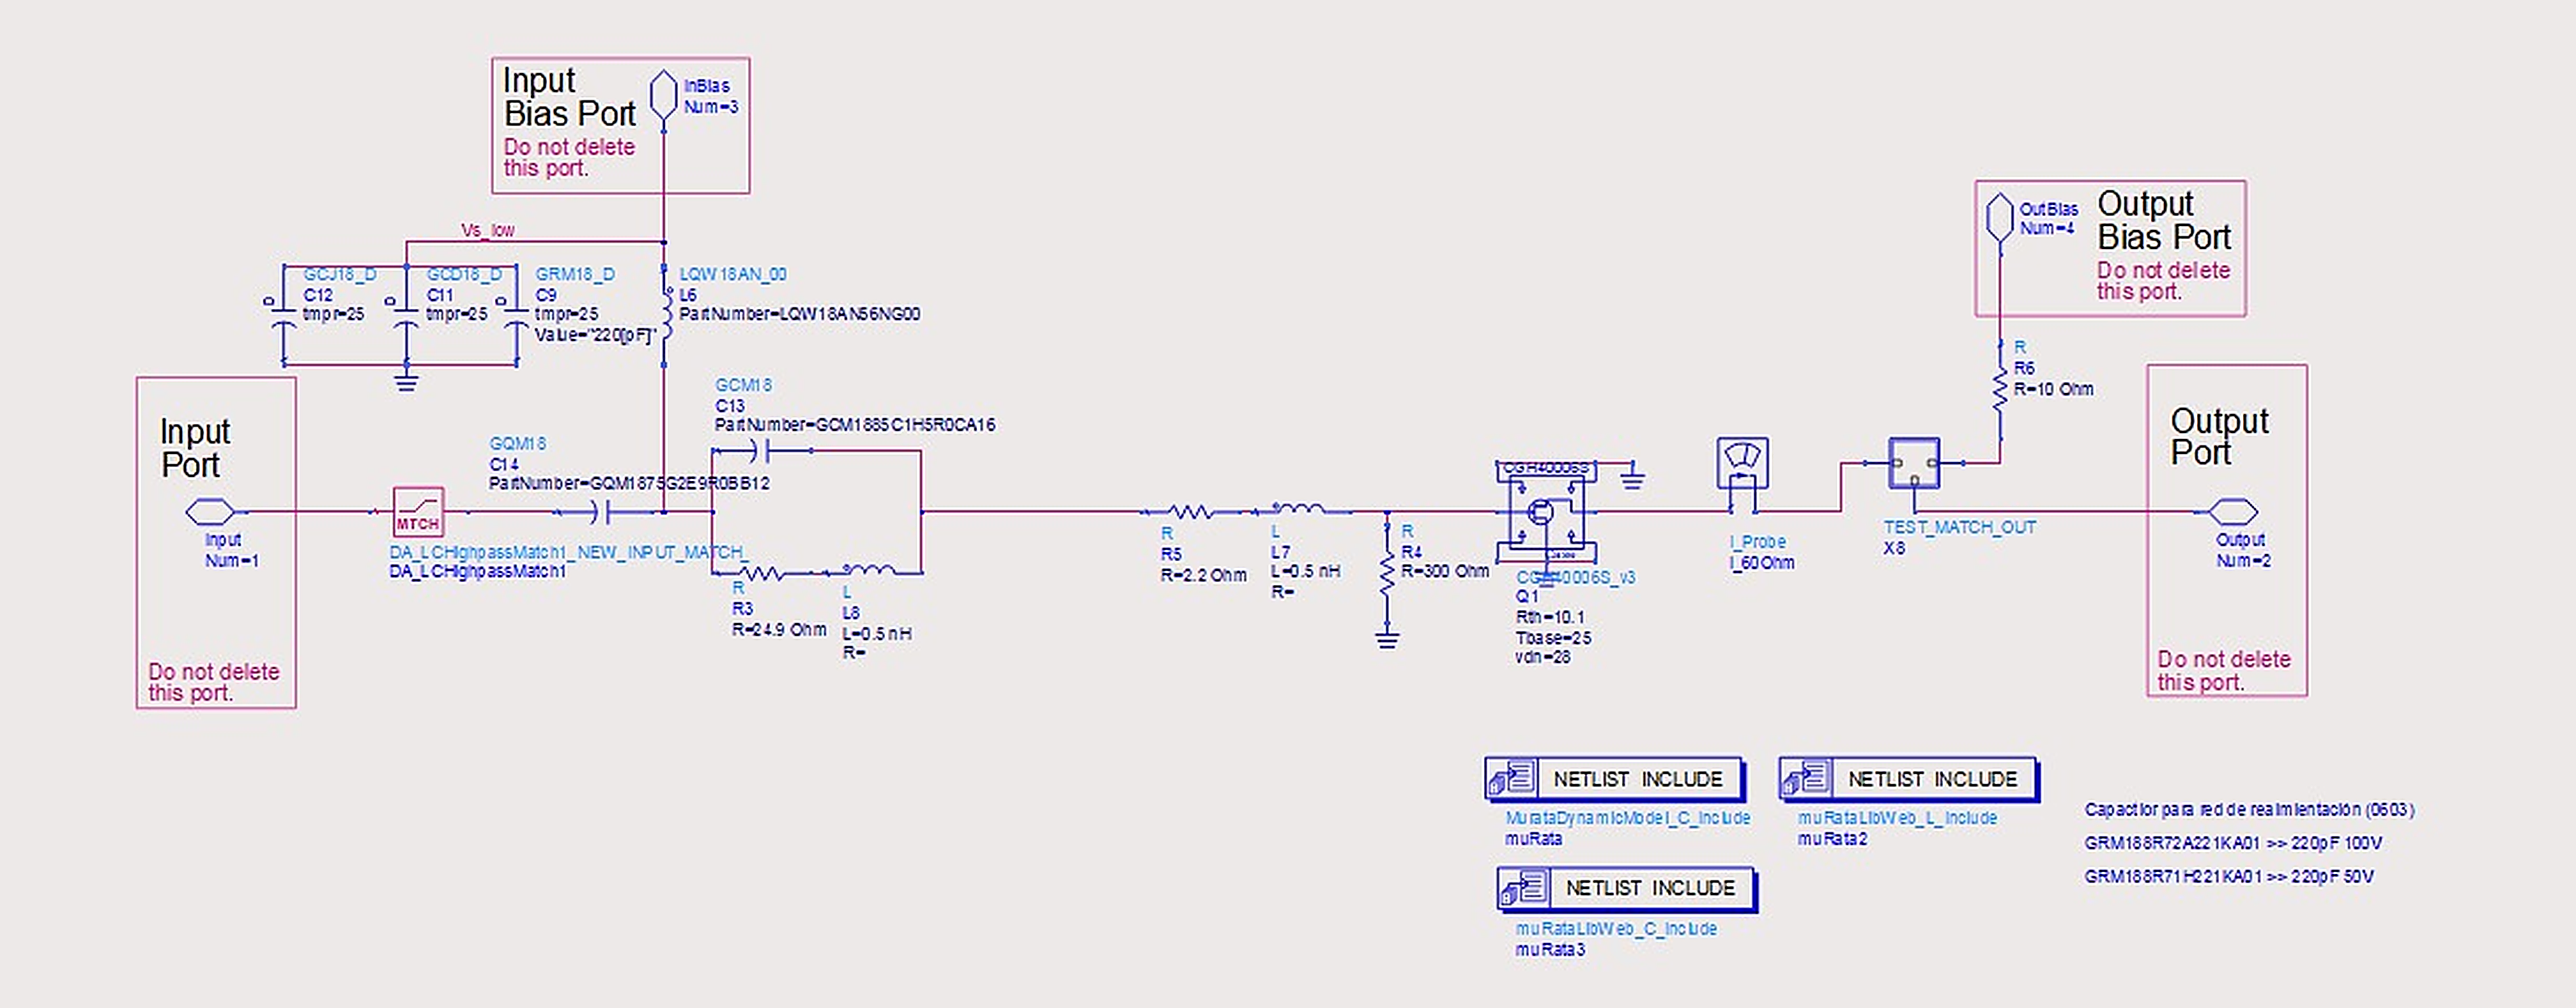
\includegraphics[width=\linewidth]{Figures/07/pa_ads_final.png}
    \caption{Esquemático de la red de estabilidad final, incorporada con el circuito ya prácticamente terminado, incluyendo los inductores parásitos (L7, L8) asociados a las resistencias reales de la red.}
    \label{fig:pa_ads_final}
\end{figure}

La Figura~\ref{fig:pa_ads_stability_plot} confirma el resultado de esta última revisión: tanto $\mu_{load}$ como $\mu_{source}$ se mantienen por encima de la unidad en la totalidad de la banda simulada (0,5 a 8~GHz), verificando la estabilidad incondicional del circuito final.

\begin{figure}[H]
    \centering
    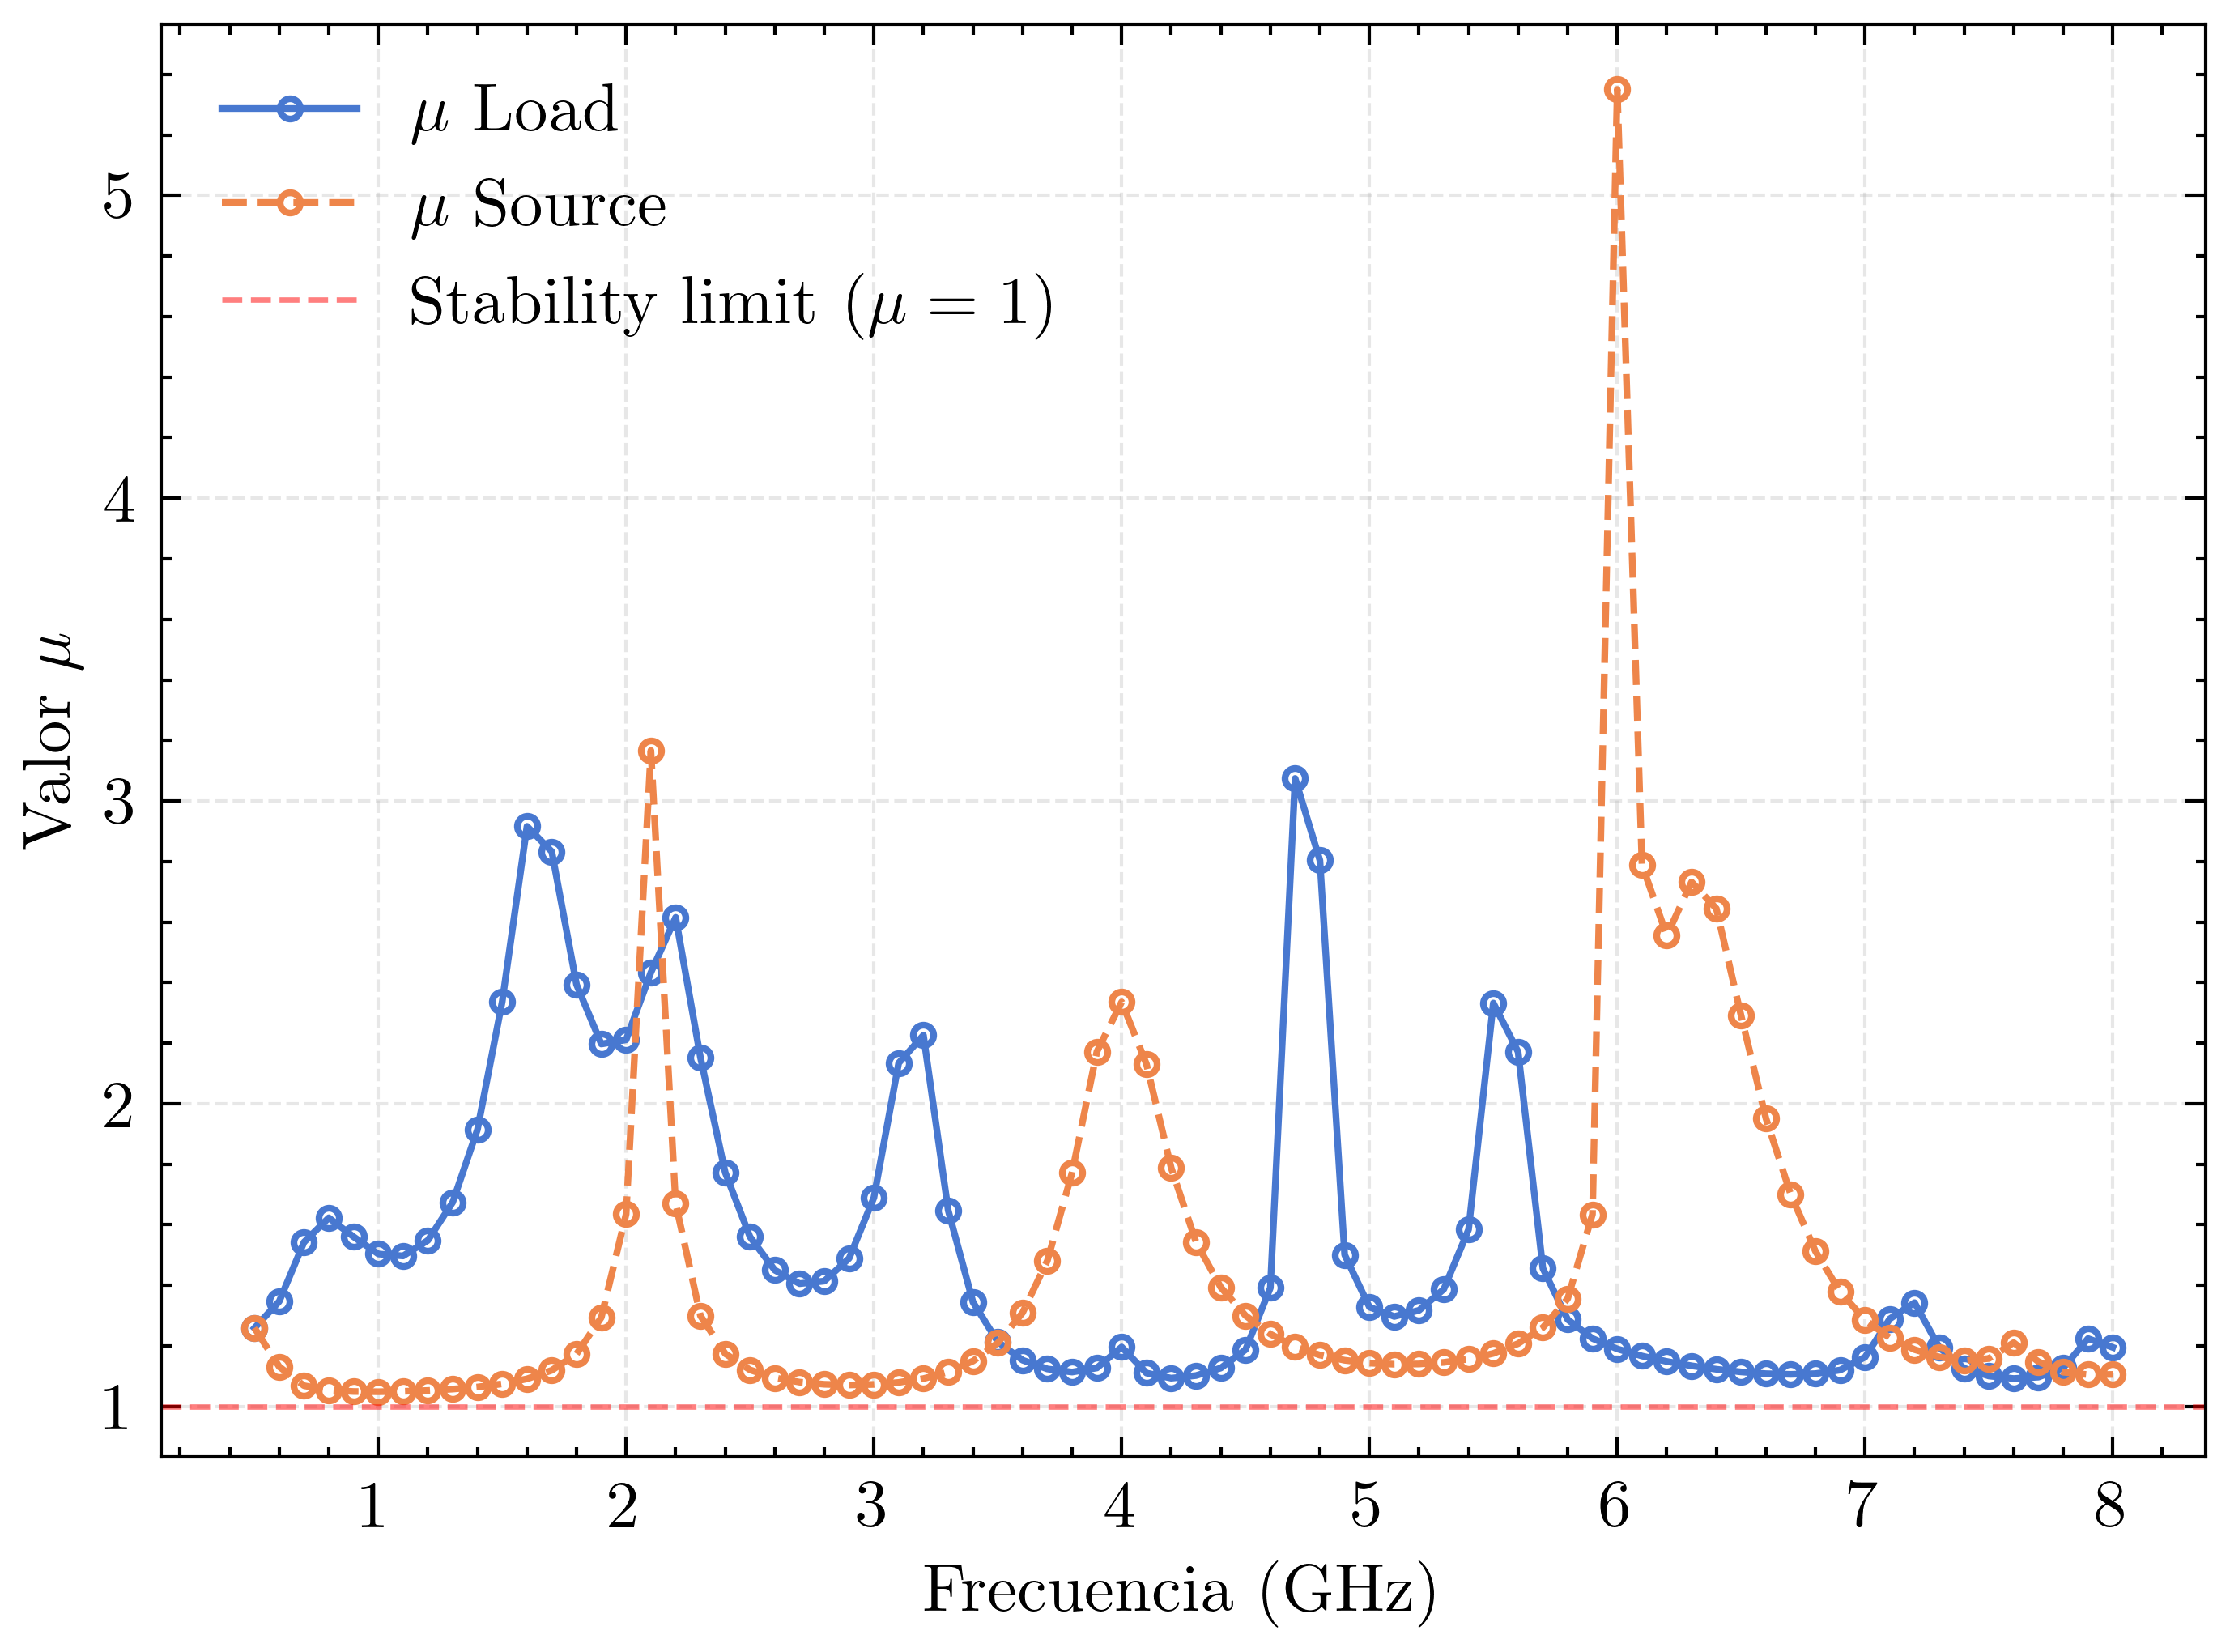
\includegraphics[width=0.6\linewidth]{Figures/07/pa_stability_plot.png}
    \caption{Factores de estabilidad $\mu_{load}$ y $\mu_{source}$ en función de la frecuencia, correspondientes a la red de estabilidad final del amplificador.}
    \label{fig:pa_ads_stability_plot}
\end{figure}

\textbf{Simulación de load-pull.} Una vez definida la red de estabilidad, se determinó la impedancia de carga que maximiza el desempeño de gran señal del transistor mediante load-pull. Con el objetivo de aislar el comportamiento del transistor de los elementos de la red de salida durante esta caracterización, el circuito de load-pull se armó de manera tal que la carga barrida se conectara directamente a los puertos del transistor, sin la influencia de las líneas de transmisión ni los capacitores que posteriormente conformarían la red de adaptación física. El valor de la impedancia de carga seleccionado fue de $Z_L=(24.1 + j52) \,\Omega$. La Figura~\ref{fig:pa_loadpull} ilustra el diagrama de Smith con los contornos obtenidos mediante load-pull.

\begin{figure}[H]
    \centering
    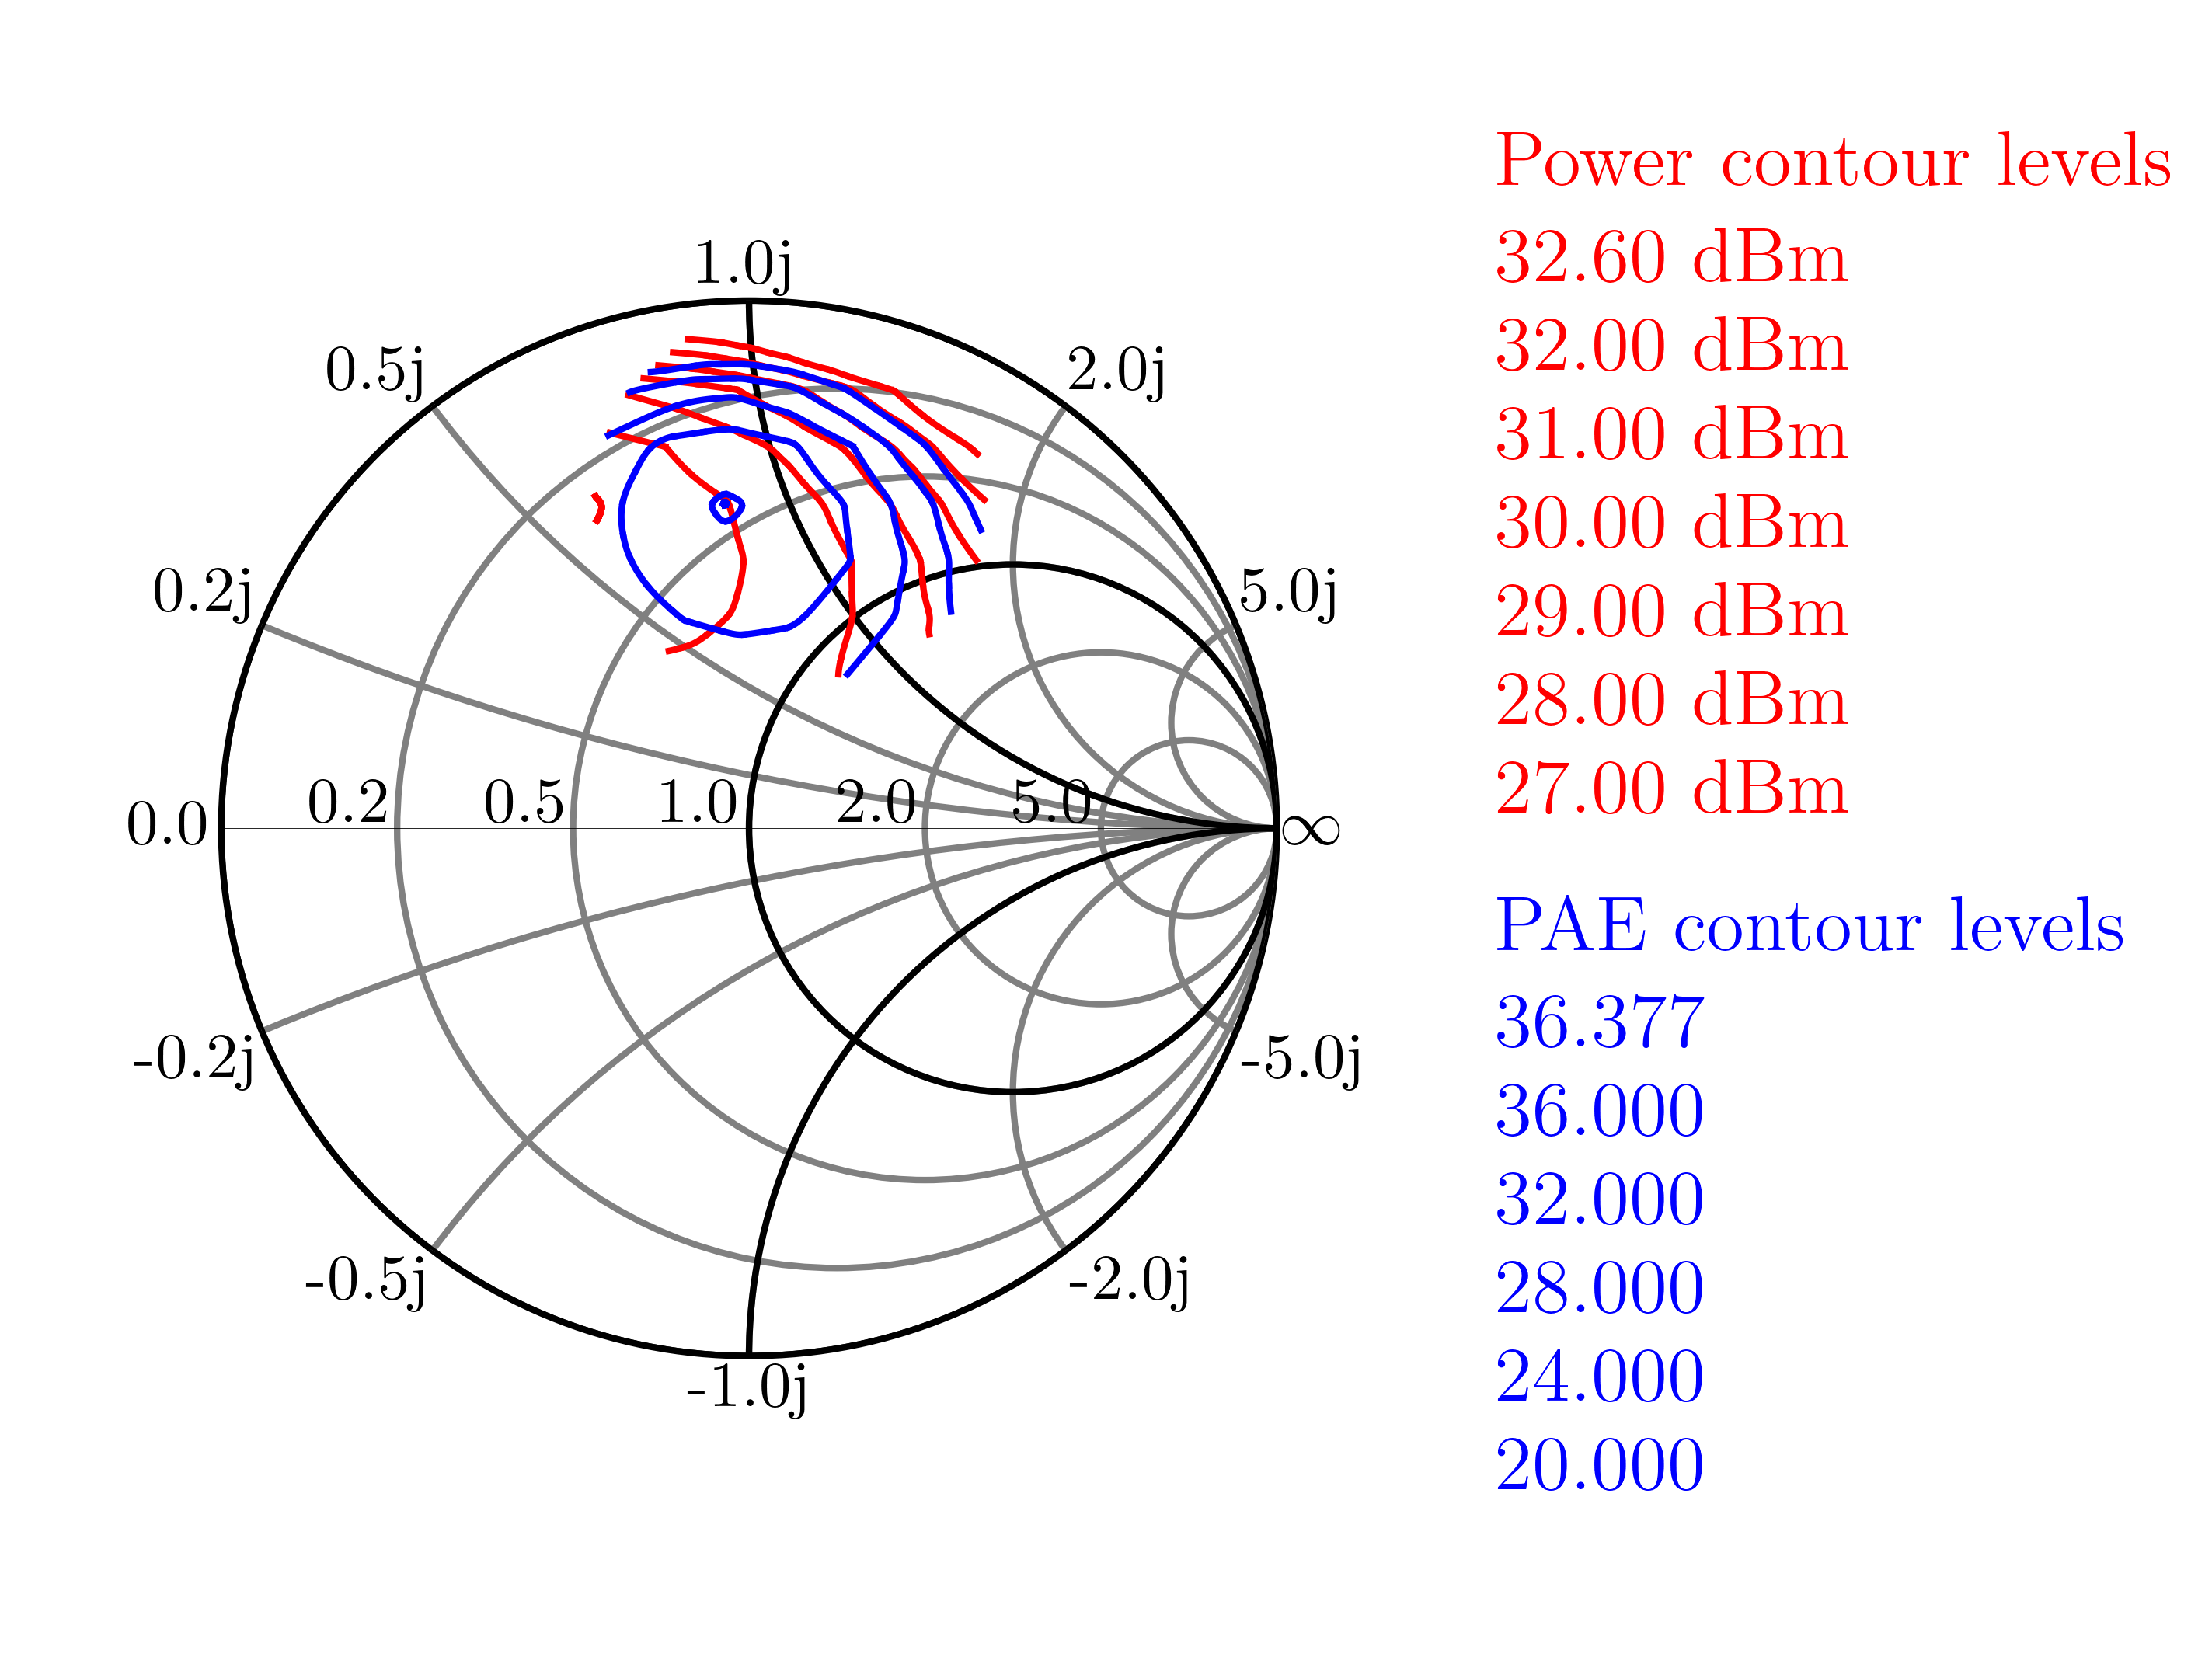
\includegraphics[width=0.9\linewidth]{Figures/07/pa_loadpull_plot.png}
    \caption{Contornos de potencia entregada y de PAE obtenidos mediante simulación de load-pull.}
    \label{fig:pa_loadpull}
\end{figure}

Durante las primeras pruebas de load-pull, con el primer diseño de la red de estabilidad, se evaluó el efecto de reducir la potencia de excitación de entrada manteniendo fija la impedancia de carga. Al reducir la potencia de entrada, el punto de operación se desplaza dentro de la misma región de máxima ganancia y máxima eficiencia de los contornos de load-pull, aunque con una eficiencia de potencia añadida menor. Concretamente, al reducir la potencia de salida de 3~W a 2~W la eficiencia cae de aproximadamente 44\,\% a 37\,\%, sin embargo, la potencia continua que debe entregar la fuente de alimentación resulta proporcionalmente menor, de acuerdo con la relación:

\begin{equation}
    P_{fuente} = \frac{P_{out}}{\eta}
    \label{eq:potencia_fuente}
\end{equation}

lo que arroja $P_{fuente}(P_{out}=3~\,W) \approx 6,81~\,W$ frente a $P_{fuente}(P_{out}=2~\,W) \approx 5,40~\,W$. Esta observación resulta relevante para una aplicación satelital con presupuesto energético acotado, dado que evidencia que, para una misma impedancia de carga, la elección del nivel de excitación de entrada permite priorizar entre maximizar la eficiencia o minimizar la potencia total consumida de la plataforma, según el criterio de diseño que se desee adoptar.

\textbf{Selección de componentes reales y resonancias parásitas.} Sobre la base del diseño obtenido con componentes ideales, se reemplazaron los capacitores e inductores discretos por sus modelos reales de montaje superficial, provenientes de la biblioteca del fabricante muRata, empleando la biblioteca dinámica para los capacitores y la biblioteca estática para los inductores. Este reemplazo reveló que el comportamiento de dichos componentes se veía afectado por sus inductancias parásitas, las cuales provocaban resonancias en frecuencias cercanas a la de operación, e incluso por debajo de esta, con impacto directo sobre la confiabilidad del circuito: los parámetros resultantes eran muy sensibles a pequeñas variaciones tanto en la longitud de las líneas de transmisión como en los valores de los componentes, además de degradar la estabilidad y la ganancia del amplificador.

Para resolver este problema se buscaron componentes pasivos reales mediante la herramienta SimSurfing del fabricante muRata, seleccionando capacitores e inductores cuya frecuencia de autorresonancia no se encontrara próxima a la banda de operación de interés, y verificando adicionalmente su disponibilidad en stock en los proveedores Digikey y JLCPCB. Los criterios adoptados para la selección de cada componente fueron el tamaño del encapsulado (0603 o 0805), el valor nominal, la tolerancia y los valores máximos admisibles de tensión, en el caso de los capacitores, y de corriente, en el caso de los inductores.

Una vez incorporados los componentes reales seleccionados de esta manera, el circuito resultó considerablemente más robusto frente a variaciones. Durante las pruebas en el segundo diseño de la red de estabilidad, la resimulación del circuito con componentes reales resultó en una perdida de 0.4\,W respecto del diseño ideal, mientras que la eficiencia se mantuvo en un nivel similar. Adicionalmente, se observó que para un mismo tipo de componente, cuanto mayor es el encapsulado, mayores resultan los valores de sus elementos parásitos. La utilización de componentes reales puede observarse en la Figura~\ref{fig:pa_ads_final}, donde inductores y capacitores reales tienen asignado su respectivo número de parte.

\textbf{Diseño de la red de adaptación de salida.} El diseño físico de la red de adaptación de salida se inició empleando líneas de transmisión ideales, incorporando dos consideraciones particulares de diseño. En primer lugar, en lugar de emplear un inductor de choque para aislar la fuente de alimentación de la señal de radiofrecuencia, esta función se cumple mediante una línea de transmisión de 50~$\Omega$ de aproximadamente $90^\circ$ eléctricos (es decir, de longitud $\lambda/4$), la cual refleja hacia el resto de la red la baja impedancia de la fuente de alimentación como un circuito abierto en el nodo de interés a la frecuencia de operación. En segundo lugar, se incorporaron stubs en la red, dispuestos con el objetivo de presentar una impedancia de cortocircuito en las frecuencias armónicas de la señal, contribuyendo a suprimir el contenido espectral no deseado a la salida del amplificador. Posteriormente se agregaron capacitores discretos de montaje superficial, cumpliendo la función de filtros de fuente de DC y como filtro de continua sobre la línea de RF. 

\begin{figure}[H]
    \centering
    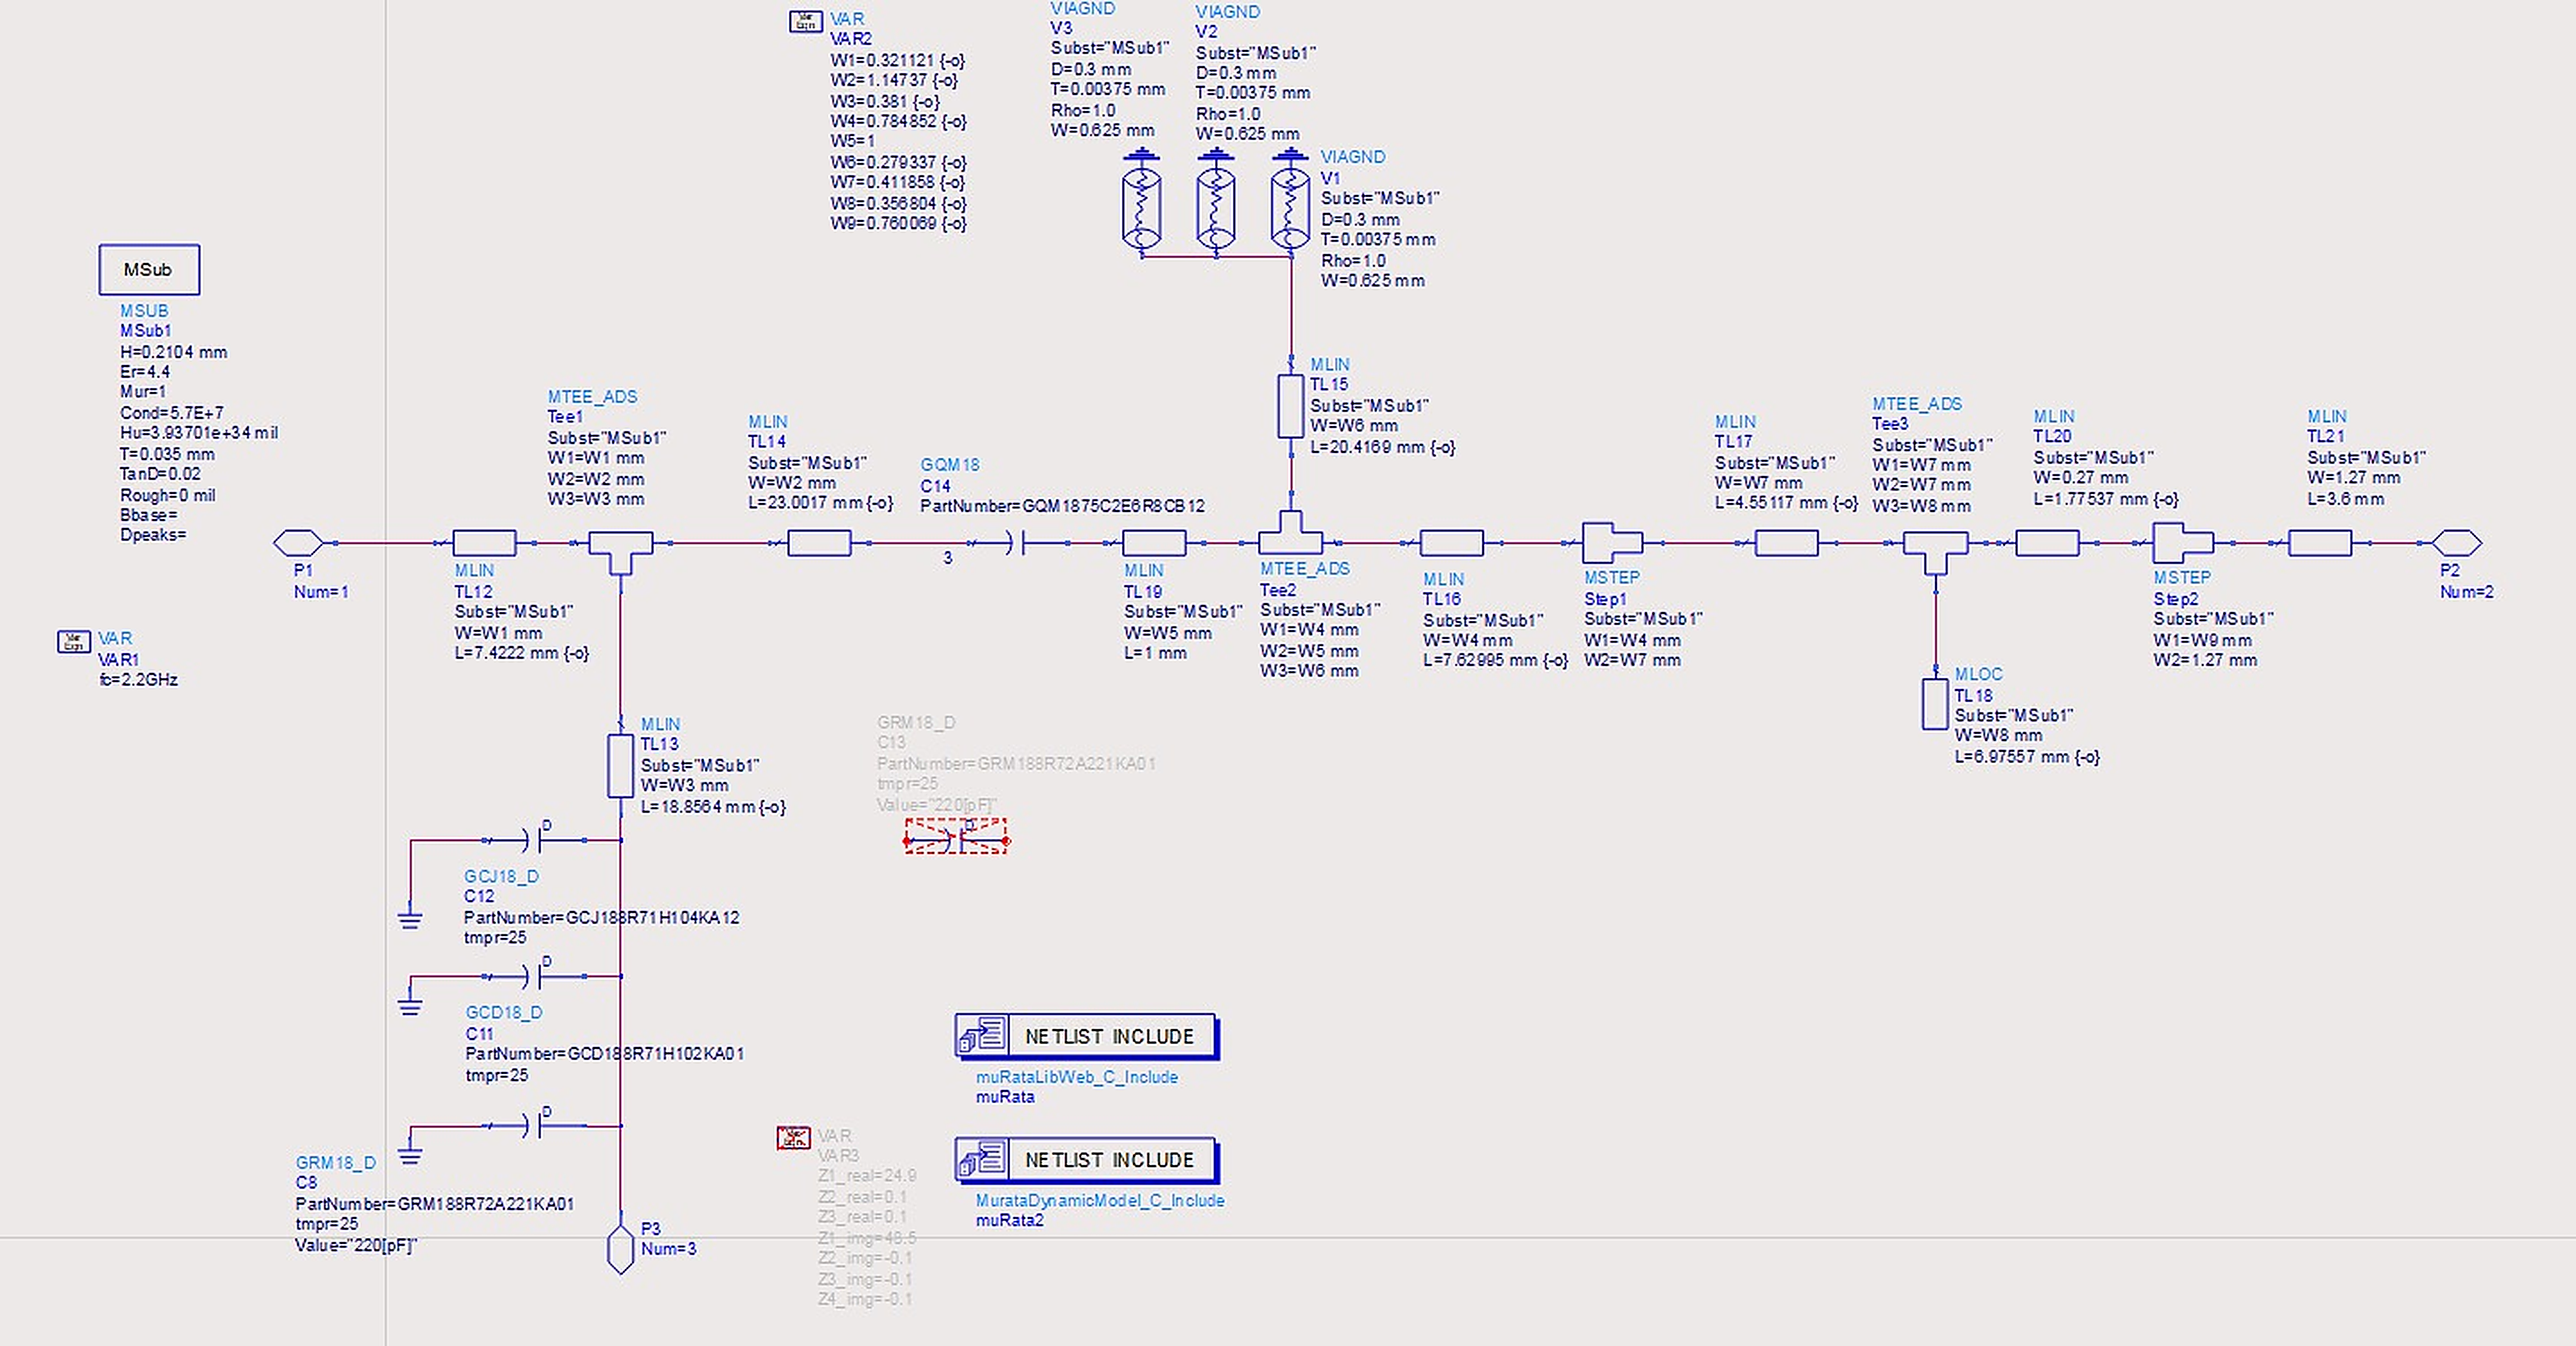
\includegraphics[width=\linewidth]{Figures/07/pa_ads_out_match.png}
    \caption{Circuito de adaptación de salida del diseño final del amplificador de potencia.}
    \label{fig:pa_match_out}
\end{figure}

\textbf{Diseño de la red de adaptación de entrada.} De manera análoga a la red de salida, el diseño físico de la red de adaptación de entrada se realizó con líneas de transmisión ideales complementadas con componentes discretos reales. La Figura~\ref{fig:pa_match_in} muestra el esquemático resultante, la cual además de adaptar, cumple la función de filtro pasa altos.

\begin{figure}[H]
    \centering
    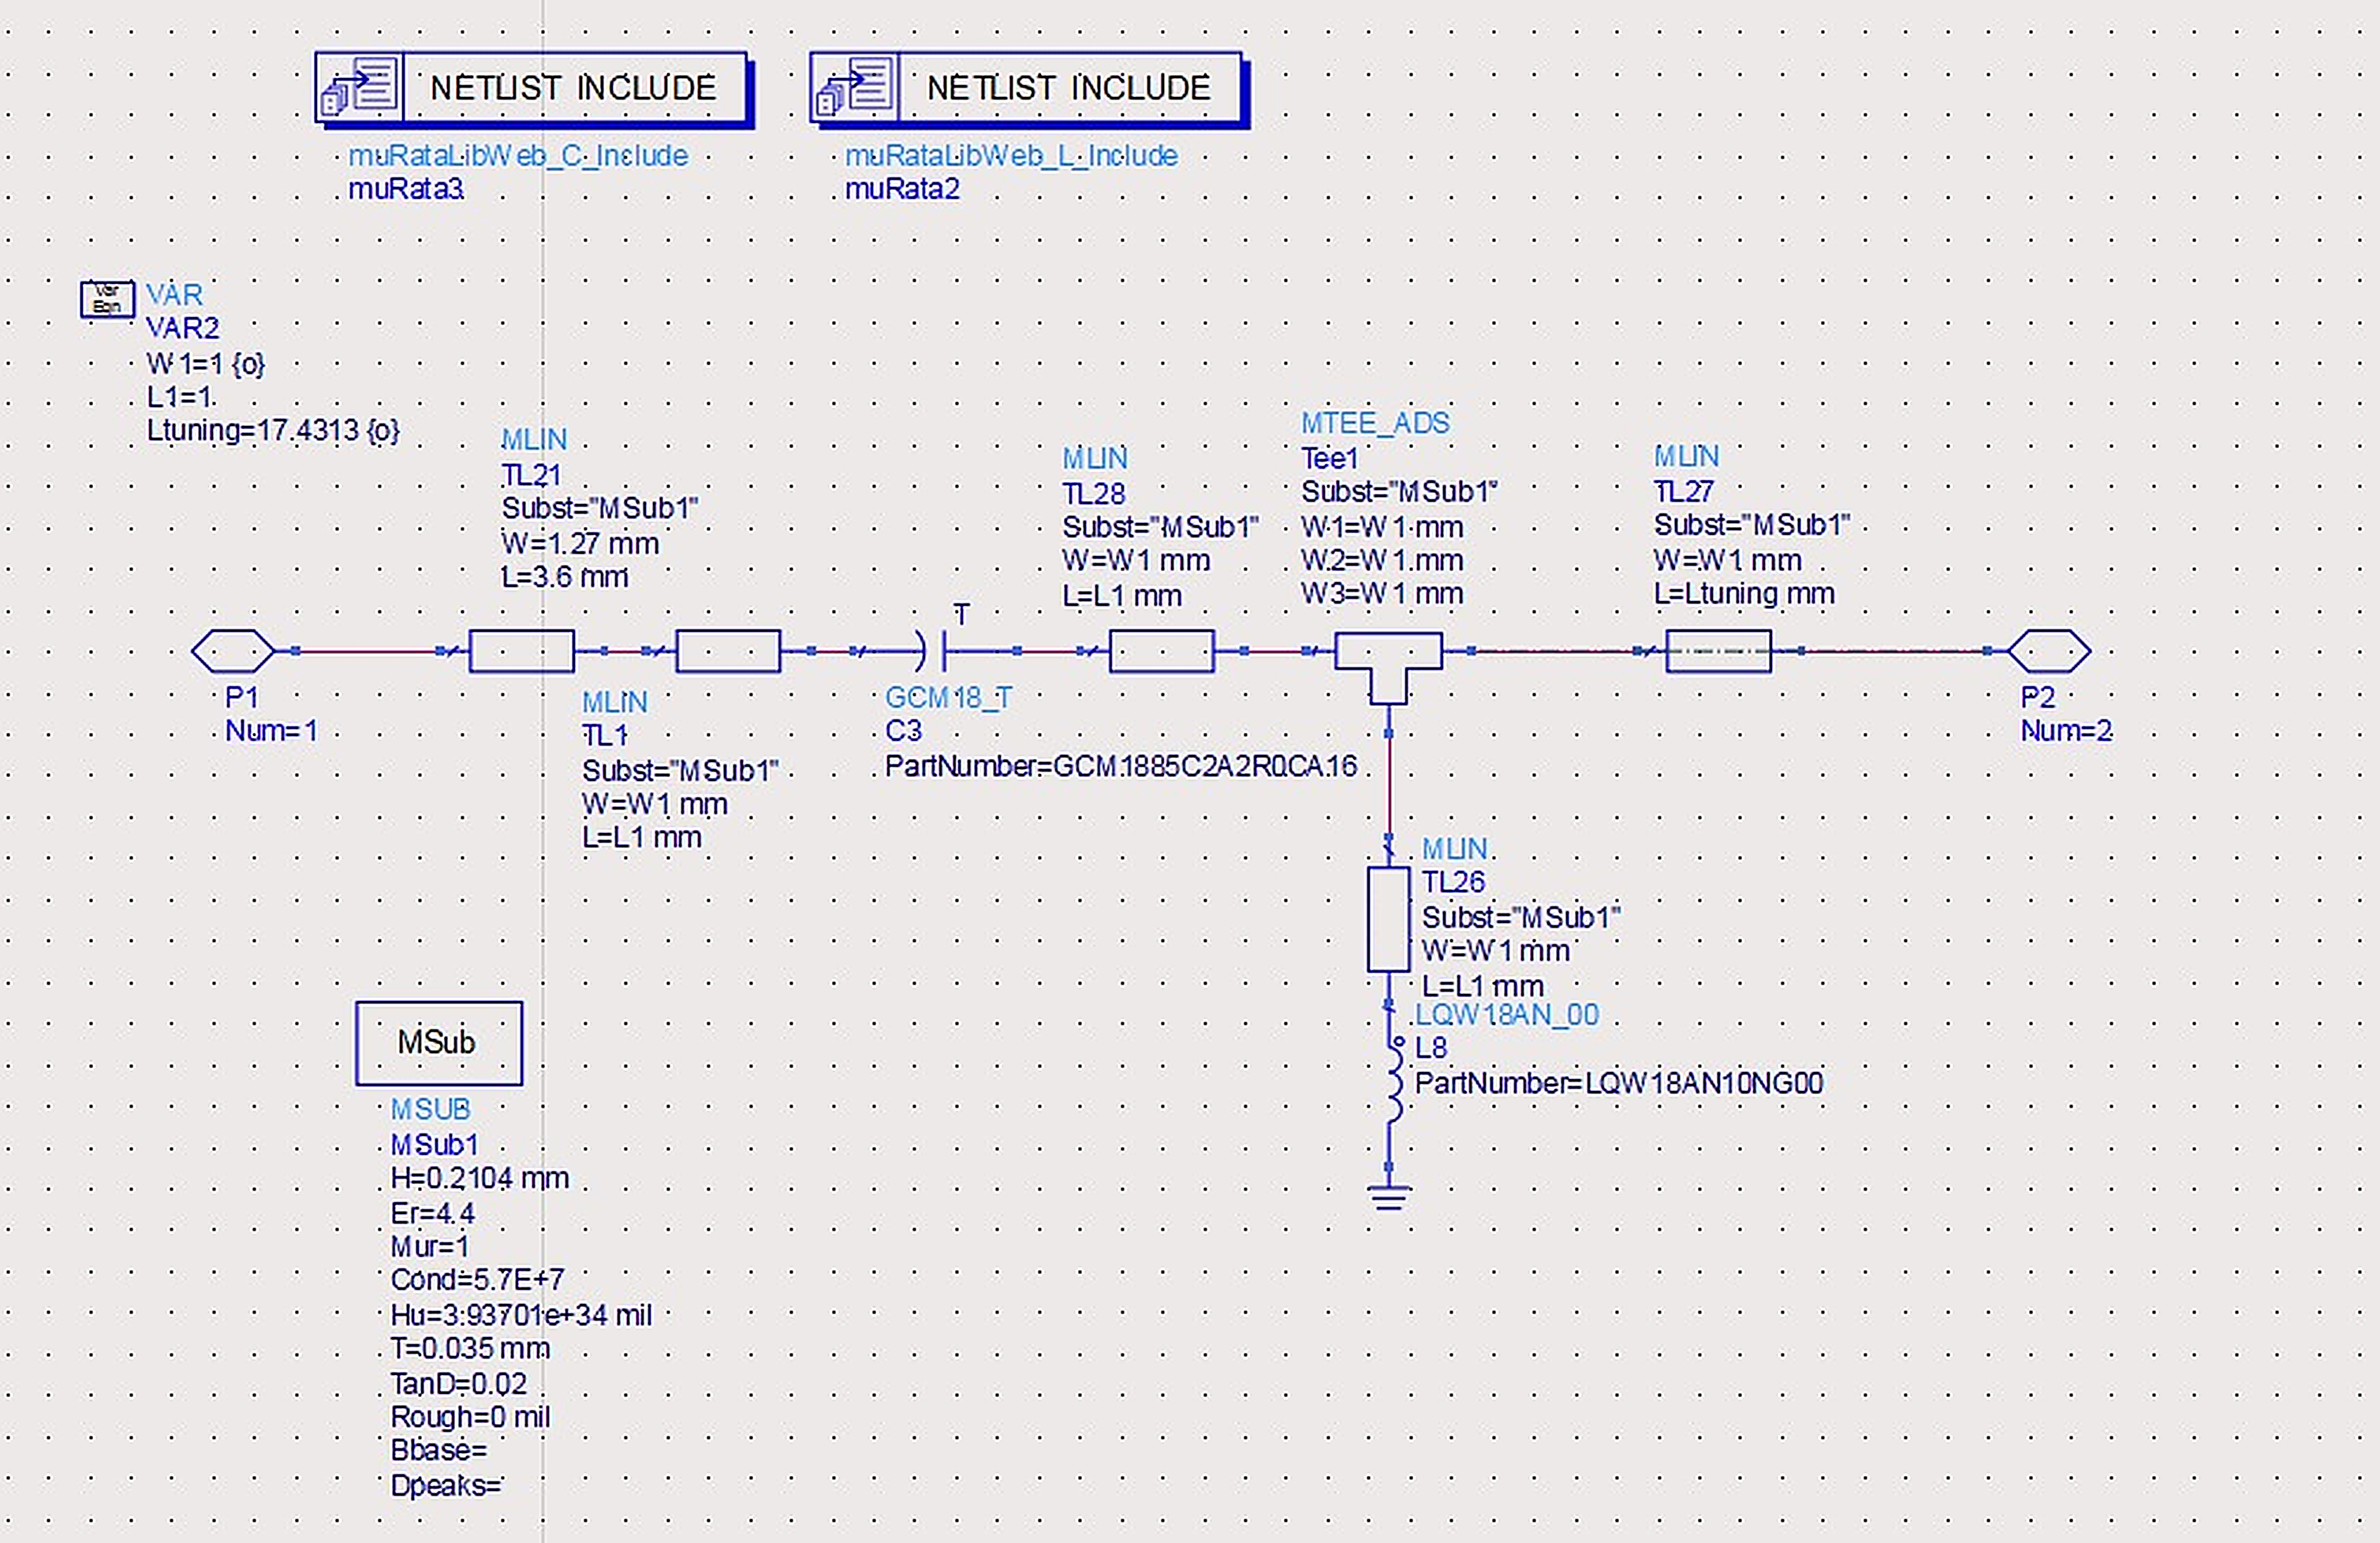
\includegraphics[width=\linewidth]{Figures/07/pa_ads_in_match.png}
    \caption{Circuito de adaptación de entrada del diseño final del amplificador de potencia.}
    \label{fig:pa_match_in}
\end{figure}

\textbf{Resultados de la optimización.} Con los componentes reales, la red de estabilidad definitiva y las redes de adaptación incorporadas, se ejecutó una nueva rutina de optimización sobre el esquemático completo, de la cual se obtuvieron los parámetros de dispersión, el contenido armónico a la salida y los parámetros de gran señal del amplificador para una potencia de entrada de 20~dBm y una tensión de alimentación de drain de 28~V.

\begin{figure}[H]
    \centering
    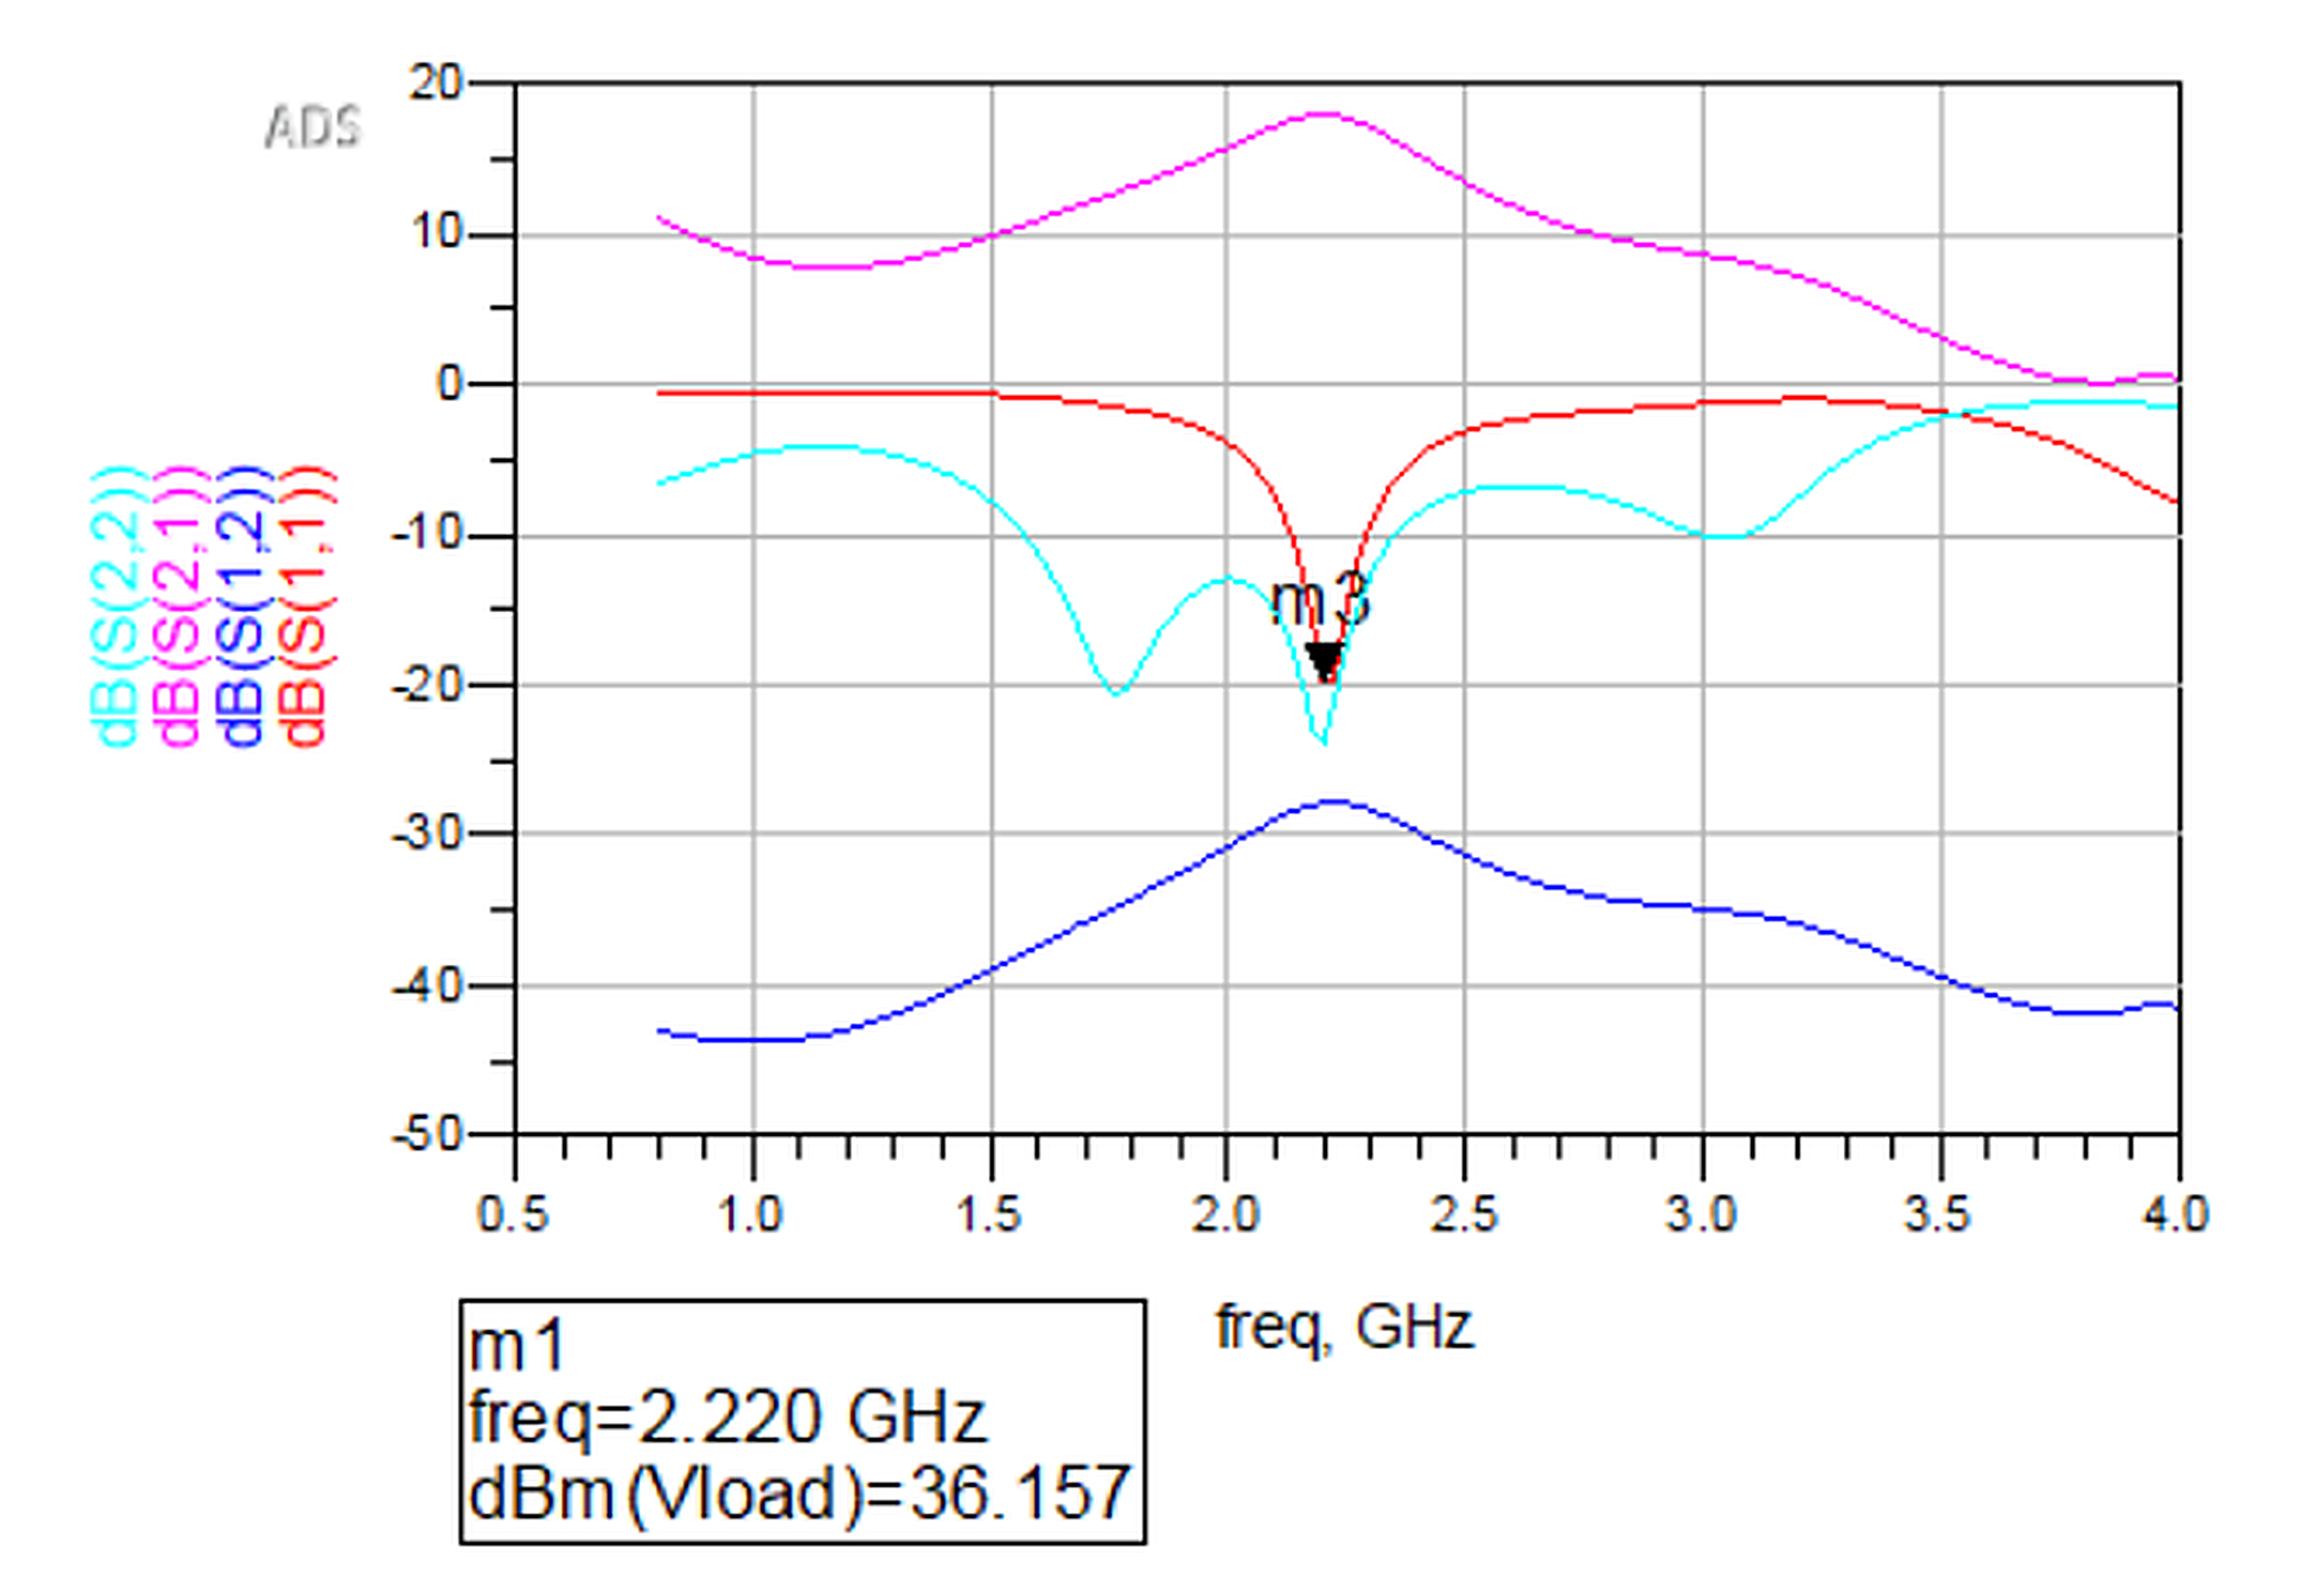
\includegraphics[width=0.75\linewidth]{Figures/07/pa_ads_sparams.png}
    \caption{Parámetros de dispersión simulados del amplificador en ADS (Pin=20\,dBm, Vdd=28\,V).}
    \label{fig:pa_ads_sparam}
\end{figure}

\begin{figure}[H]
    \centering
    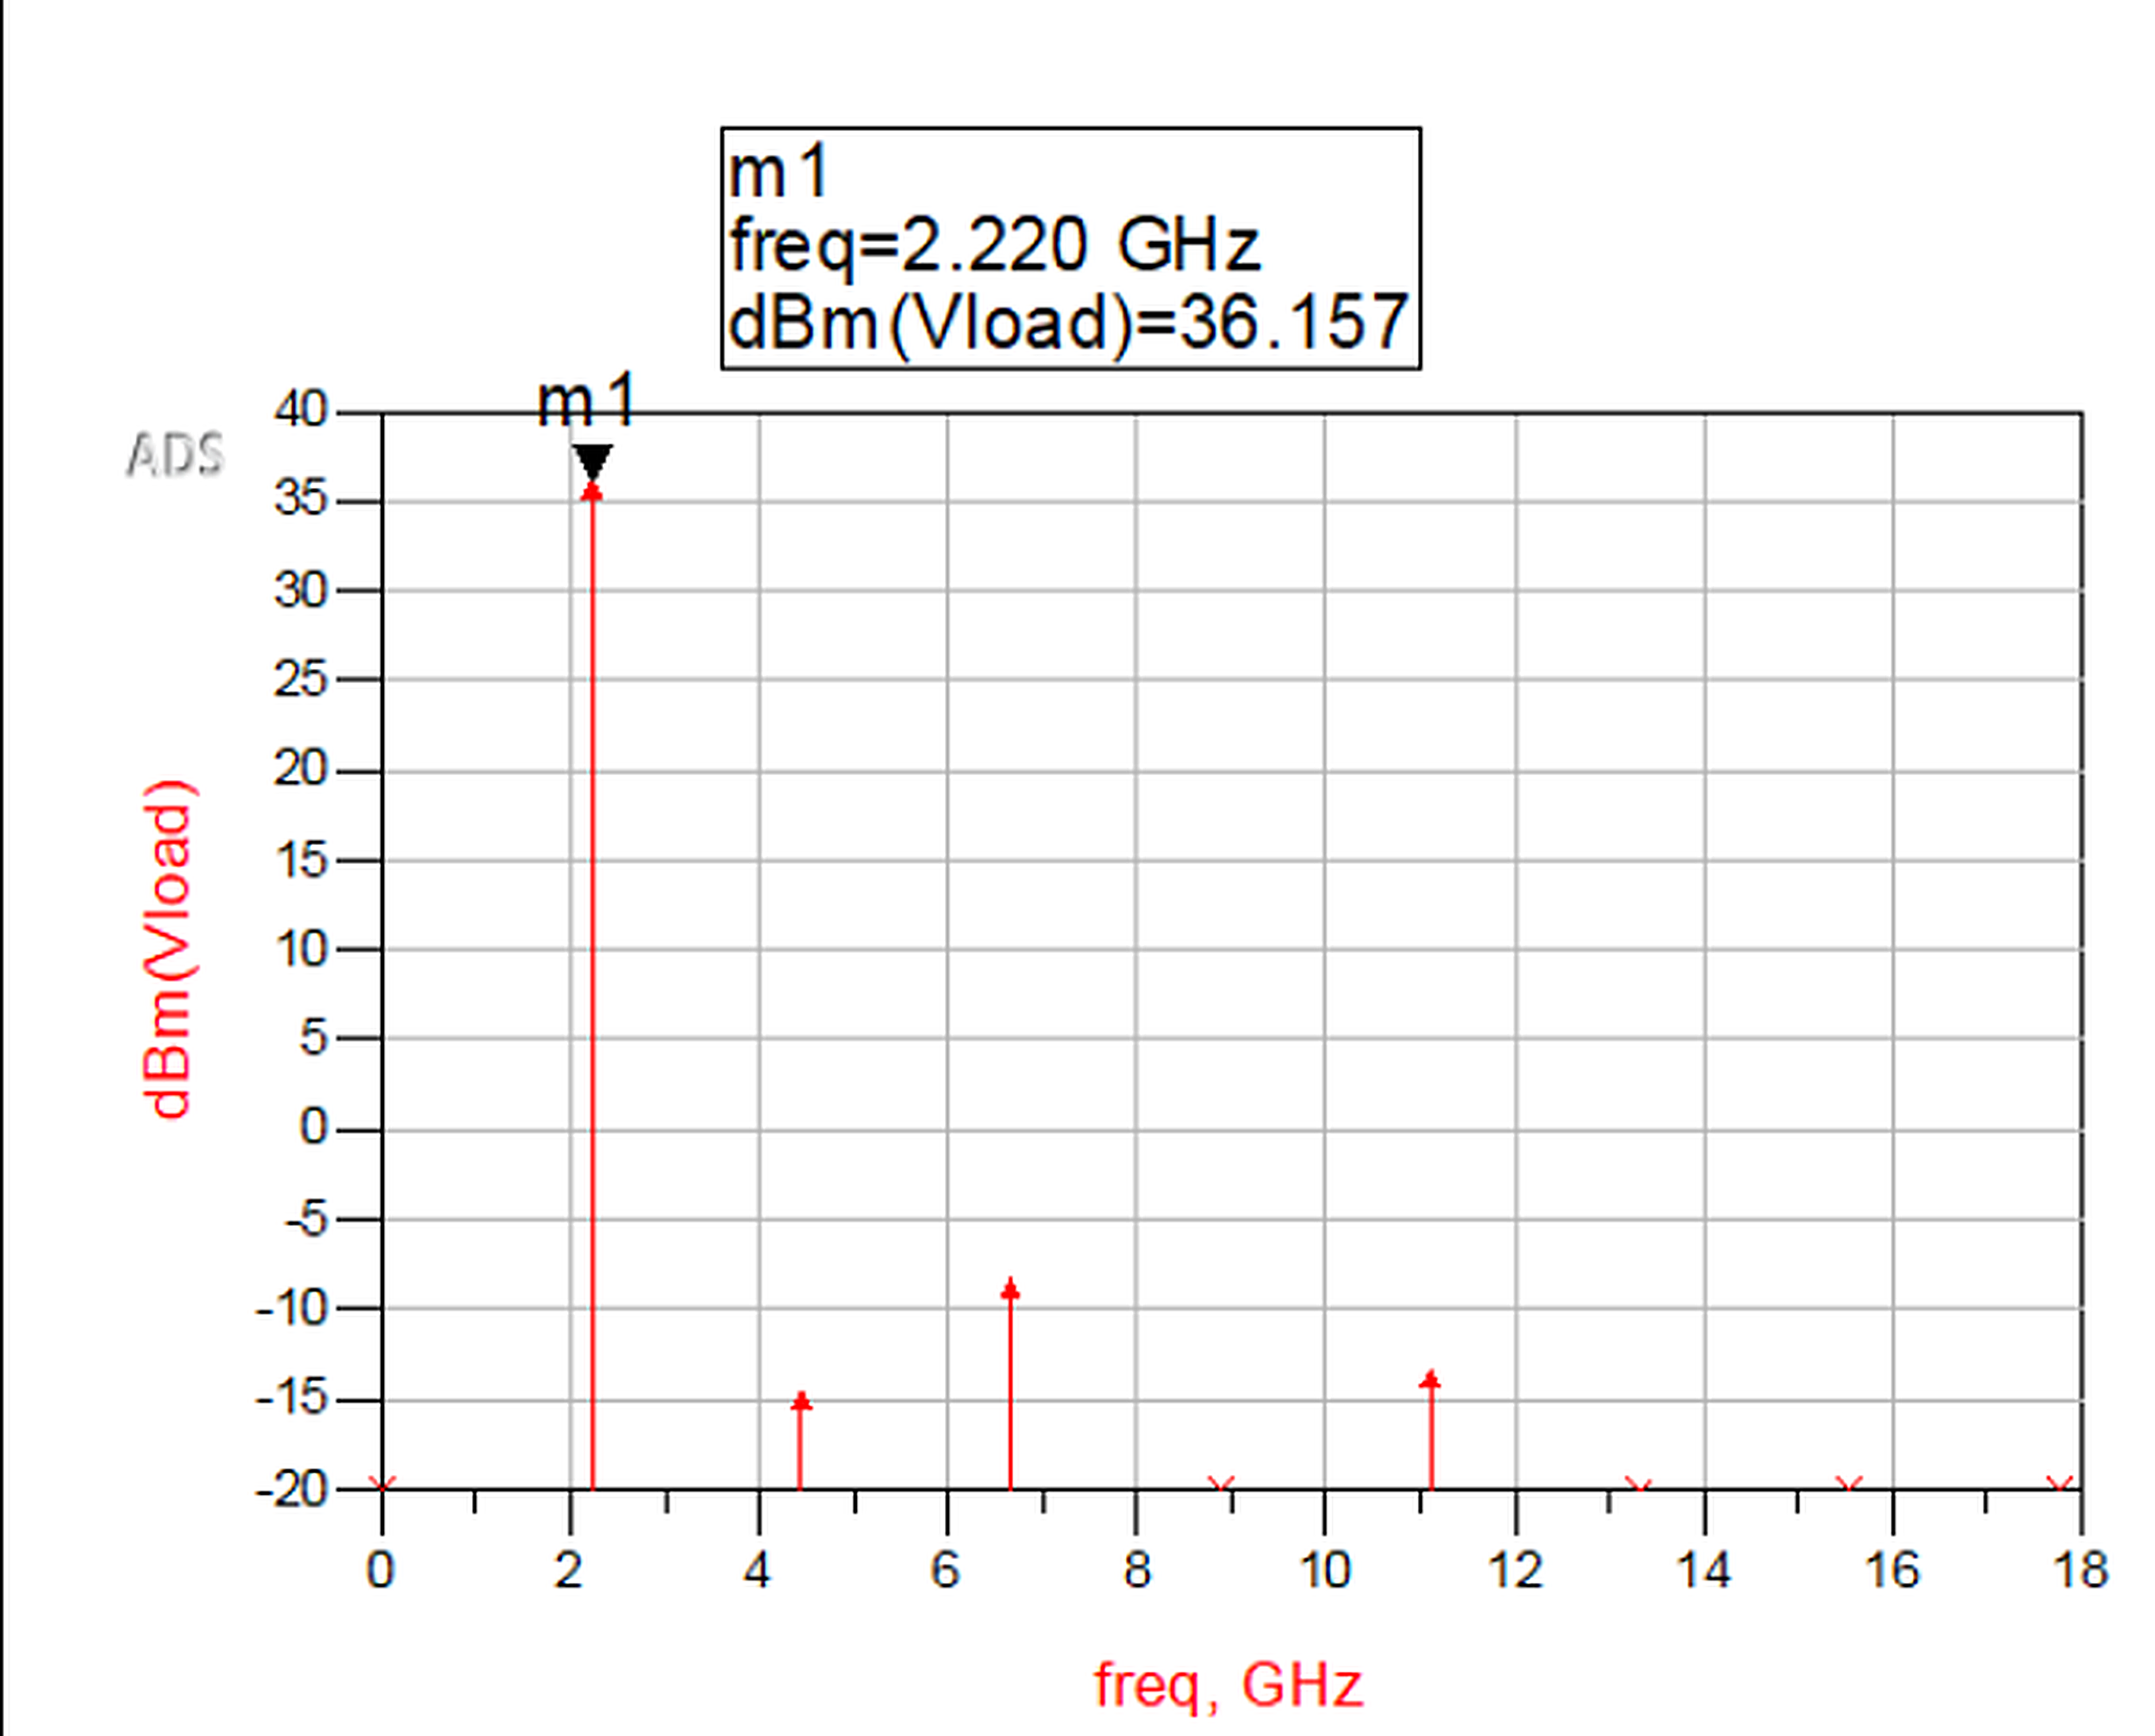
\includegraphics[width=0.7\linewidth]{Figures/07/pa_ads_harmonics.png}
    \caption{Contenido armónico simulado en la carga del amplificador (Pin=20\,dBm, Vdd=28\,V).}
    \label{fig:pa_ads_armonicos}
\end{figure}

\begin{table}[H]
    \centering
    \caption{Valores de desempeño simulados en ADS (Pin=20\,dBm, Vdd=28\,V).}
    \label{tab:pa_valores_importantes_ads}
    \begin{tabular}{lcc}
        \hline\hline
        \textbf{Parámetro}   & \textbf{Valor}  & \textbf{Unidad} \\
        \hline
        $P_{out}$            & 36,157          & dBm             \\
        Ganancia             & 16,157          & dB              \\
        PAE                  & 50,910          & \%              \\
        Eficiencia de drain  & 52,149          & \%              \\
        \hline\hline
    \end{tabular}
\end{table}

Los resultados obtenidos a nivel esquemático se consideraron satisfactorios respecto de los objetivos de diseño del Cuadro~\ref{tab:objetivos_diseno}, por lo que se procedió hacia la etapa de diseño físico del circuito impreso.

\subsection{Diseño de PCB}

\subsection{Verificación electromagnética}

% -----------------------------------------------------------------------------------------------%
\subsection{Radioenlace satelital} \label{sec:radioenlace}
Una vez determinada la potencia de salida alcanzable por el amplificador desarrollado, se realizó un análisis de radioenlace satelital o \textit{link budget}, herramienta analítica que permite cuantificar la potencia de la señal a lo largo de todo el trayecto de transmisión y comparar el nivel de señal recibido contra el umbral mínimo necesario para satisfacer la tasa de error de bit (\textit{bit error rate}, BER) requerida por la misión. El objetivo de este análisis fue determinar, a partir de la potencia de salida obtenida, qué esquemas de modulación M-PSK resultan viables para el enlace y bajo qué condiciones de elevación de la antena terrena, cerrando de esta manera el ciclo de diseño entre el desempeño real del hardware desarrollado y los requisitos de la misión.

El análisis se fundamenta en la evaluación de la densidad de flujo de potencia y las propiedades del medio físico de propagación, como fue propuesto por Friis \textbf{[REF. FRIIS]}: una antena transmisora que radia una potencia $P_t$ con una ganancia de directividad $G_t$ produce, a una distancia $d$, una densidad de flujo de potencia $S$ dada por:

\begin{equation}
    S = \frac{P_t G_t}{4\pi d^2} = \frac{\text{EIRP}}{4\pi d^2}
    \label{eq:densidad_flujo}
\end{equation}

donde EIRP representa la potencia isotrópica radiada equivalente y constituye, en términos del receptor, una cantidad equivalente a la de una fuente isotrópica ideal que produce la misma densidad de flujo en la dirección considerada. En un escenario real, la potencia entregada a la antena se ve degradada por las pérdidas mecánicas y dieléctricas en las líneas de transmisión intermedias entre el amplificador de potencia desarrollado y el puerto de alimentación de la antena, de modo que, expresado logarítmicamente, el EIRP se calcula como:

\begin{equation}
    \text{EIRP [dBW]} = P_t \text{ [dBW]} - L_{tx} \text{ [dB]} + G_{tx} \text{ [dBi]}
    \label{eq:eirp_analitico}
\end{equation}

aquí $L_{tx}$ representa las pérdidas de conducción del transmisor y $G_{tx}$ la ganancia de la antena del satélite. La potencia captada por el receptor, en este caso la estación terrena, depende de la apertura efectiva de su antena receptora ($A_e$), la cual está intrínsecamente ligada a su ganancia de directividad $G_{rx}$ y a la longitud de onda de la portadora $\lambda$ mediante la relación geométrica:

\begin{equation}
    A_e = \frac{G_{rx}\lambda^2}{4\pi}
    \label{eq:apertura_ef}
\end{equation}

de manera que la potencia disponible en los terminales del receptor ($P_r$) toma la forma de la ecuación de transferencia de Friis:

\begin{equation}
    P_r = S A_e = P_t G_t G_{rx} \left( \frac{\lambda}{4\pi d} \right)^2
    \label{eq:friis_formal}
\end{equation}

Al invertir el término entre paréntesis elevado al cuadrado en \eqref{eq:friis_formal}, se obtiene lo que se define como la pérdida de espacio libre (\textit{free space-path loss}, FSPL), magnitud que corresponde formalmente a una ganancia menor a la unidad y representa la atenuación debida a la expansión del frente de onda en el espacio sin involucrar disipación física de energía, que responde a:

\begin{equation}
    L_{FSPL} \text{ [dB]} = 20 \log_{10}\left( \frac{4\pi d}{\lambda} \right)
    \label{eq:fsl_formal}
\end{equation}

A diferencia de los enlaces terrestres fijos, la distancia $D$ en una órbita terrestre baja (LEO) es dinámicamente dependiente del ángulo de elevación de la antena ($\epsilon$) orientado hacia el satélite desde la estación terrena. Un modelo ilustrativo que ayuda a calcular esta distancia se presenta en la Figura~\ref{fig:slant_range}, donde C es el centro de la Tierra, A la posición de la antena en la superficie terrestre, S la posición del satélite en órbita a una altura $h$ y $R_E$ es el radio terrestre medio (6378~km).

\begin{figure}[H]
    \centering
    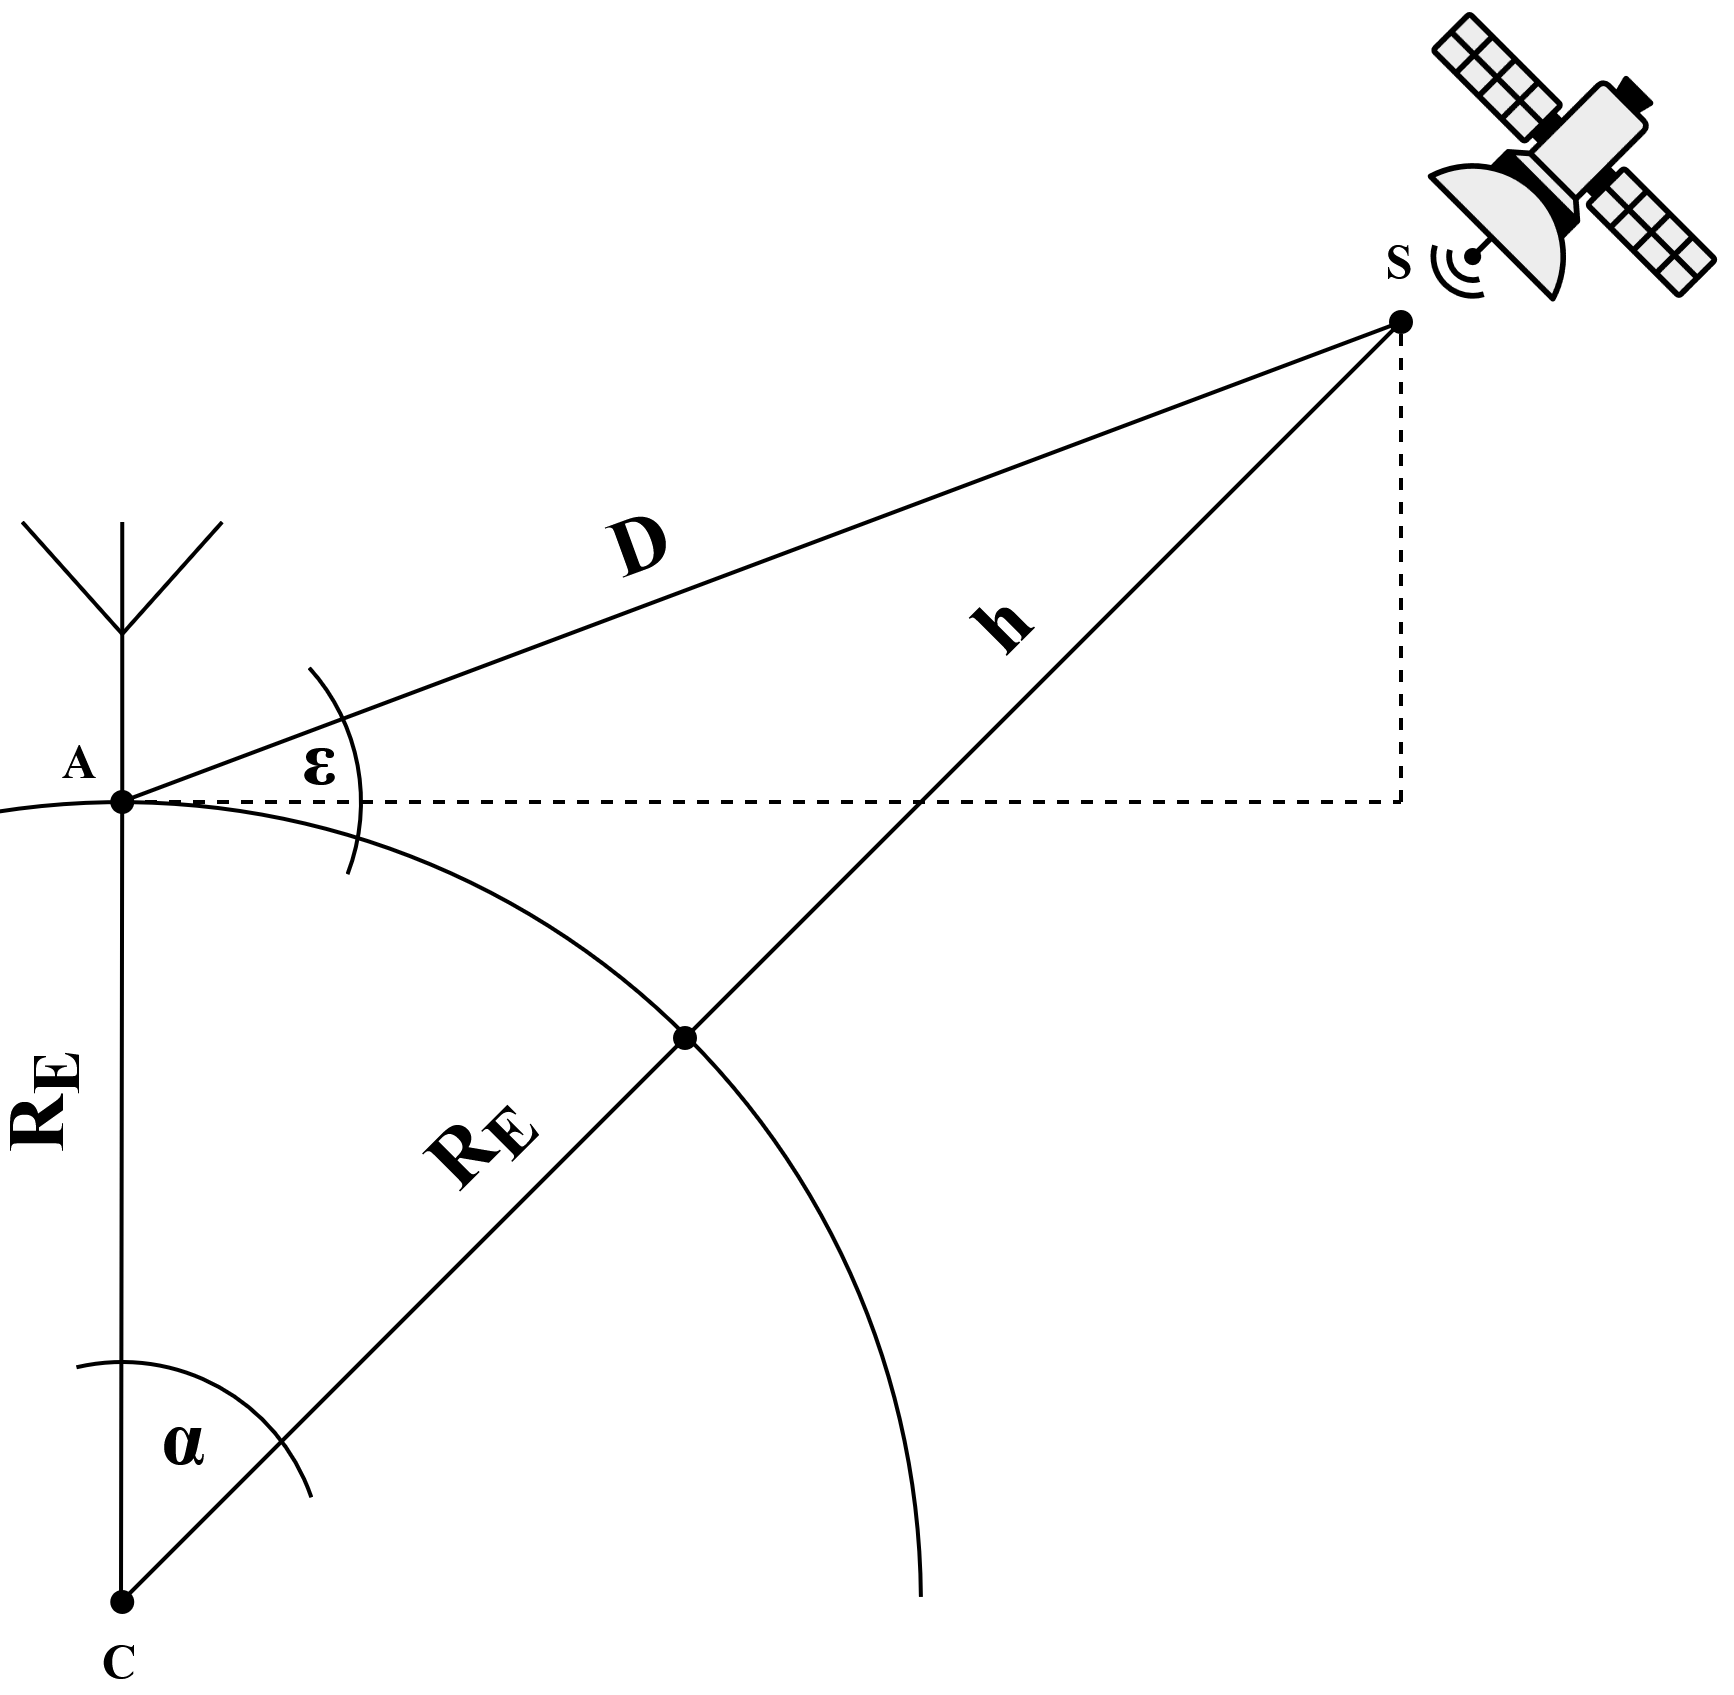
\includegraphics[width=0.7\linewidth]{Figures/07/slant_range.png}
    \caption{Modelo matemático para el cálculo de la distancia D en función del ángulo de elevación $\epsilon$.}
    \label{fig:slant_range}
\end{figure}

Utilizando la ley de los cosenos sobre la geometría esférica de la Tierra, la distancia del enlace se modela rigurosamente como:

\begin{equation}
   (R_E+h)^2 = R_E^2 + D^2 - 2\,R_E\,D\,\cos(\epsilon + \pi/2)
    \label{eq:ley_cos}
\end{equation}

Reemplazando $\cos(\epsilon+\pi/2)$ por $-\text{sen}(\epsilon)$, luego resolviendo la ecuación cuadrática para la variable $D$ y operando matemáticamente se obtiene la expresión:

\begin{equation}
    D(\epsilon) = \sqrt{(R_E + h)^2 - (R_E \cos\epsilon)^2} - R_E \sin\epsilon
    \label{eq:geometria_orbita}
\end{equation}

Como las pérdidas de espacio libre no contemplan efectos disipativos, se deben incluir en el balance de potencias las pérdidas debidas a la atmósfera y las deficiencias mecánicas de apuntamiento de las antenas, factores que, a diferencia de la FSPL, corresponden a pérdidas resistivas reales del trayecto y que se consolidan en la pérdida total de trayecto ($L_{path}$):

\begin{equation}
    L_{path}(\epsilon) \text{ [dB]} = L_{FSL}(\epsilon) + L_{point} + L_{atm}
    \label{eq:pérdidas_totales}
\end{equation}

Consecuentemente, el nivel de señal recibida (\textit{received signal level}, RSL) en función del ángulo de elevación, análogo a la diferencia entre el EIRP y la pérdida total de trayecto corregida por la ganancia neta de recepción, se determina mediante:

\begin{equation}
    \text{RSL}(\epsilon) \text{ [dBW]} = \text{EIRP} - L_{path}(\epsilon) + G_{rx} - L_{rx}
    \label{eq:rsl_formal}
\end{equation}

% ------------------------------------------------------------------------ %
\subsubsection{Modelado del ruido y calidad del enlace}
La viabilidad del enlace digital no se limita a la amplitud de la portadora recibida, sino a su relación respecto a la densidad espectral de potencia de ruido térmico presente en el sistema ($N_0$), modelado como ruido blanco gaussiano aditivo. En sistemas terrestres, este ruido suele caracterizarse mediante la figura de ruido del receptor referida a una temperatura estándar de 290\,K, sin embargo, en estaciones terrenas de comunicaciones satelitales la antena recibe directamente el ruido de cielo, sustancialmente menor a 290\,K, por lo cual resulta más preciso emplear una temperatura total de sistema en lugar de una figura de ruido equivalente. Bajo este criterio, la temperatura total de ruido del sistema receptor ($T_{sys}$) se descompone aditivamente de acuerdo con el teorema de uniones en cascada, simplificado para los componentes críticos del segmento terreno:

\begin{equation}
    T_{sys} = T_{ant} + T_{LNA}
    \label{eq:tsys}
\end{equation}

donde $T_{ant}$ es la temperatura de ruido equivalente de la antena, que captura la radiación de fondo cósmico y el ruido térmico terrestre captado por los lóbulos secundarios, y $T_{LNA}$ es la temperatura de ruido efectiva referida a la entrada del amplificador de bajo ruido. La densidad espectral de ruido resultante se expresa logarítmicamente como:

\begin{equation}
    N_0 \text{ [dBW/Hz]} = k_{dB} + 10 \log_{10}(T_{sys})
    \label{eq:n0_log}
\end{equation}

% TODO: se omitieron las ecuaciones eb/n0 (eq:ebn0_rb y eq:ebn0_bw) presentes en el
% archivo original entre esta ecuación y la siguiente, deben reincorporarse tal
% como estaban en 07-2-Radioenlace.tex al integrar este archivo al documento final.

donde el único parámetro de la cadena de transmisión digital que interviene en la ecuación es la tasa de bits $R_b$, con independencia de cómo esta haya sido determinada. En sistemas con asignación espectral rígida, $R_b$ no constituye un parámetro libre sino una cantidad derivada del ancho de banda ocupado ($BW$) y de las características del esquema de modulación. La tasa de símbolos (\textit{symbol rate}, $R_s$) en baudios se deduce a partir del factor de roll-off $\alpha$ del filtro de coseno realzado empleado para conformar el espectro, dado que la relación entre el ancho de banda ocupado y la tasa de símbolos para este tipo de filtrado responde a:

\begin{equation}
    R_s = \frac{BW}{1 + \alpha}
    \label{eq:rs_bw}
\end{equation}

A partir de la eficiencia espectral del esquema de modulación lineal M-PSK implementado, la tasa de bits efectiva queda determinada por la cantidad de bits por símbolo ($\log_{2}M$):

\begin{equation}
    R_b = R_s \log_{2}(M) = \frac{BW}{1 + \alpha} \log_{2}(M)
    \label{eq:rb_deducido}
\end{equation}

de modo que, bajo un ancho de banda constante, el aumento en el orden de la modulación $M$ incrementa la tasa de transmisión a costa de una reducción proporcional en el $E_b/N_0$ disponible por bit, según se desprende de sustituir \eqref{eq:rb_deducido} en la expresión de $E_b/N_0$ en función de $R_b$.

El valor de $[E_b/N_0]_{req}$ que interviene en el criterio de cierre del enlace no es un parámetro arbitrario, sino que depende exclusivamente de dos factores: el esquema de modulación digital empleado y la tasa de error de bit (BER) objetivo de la misión. Esta dependencia se establece a través de la función de error complementaria gaussiana, comúnmente expresada mediante la función $Q(z)$, que es la herramienta analítica para poder vincular la relación señal a ruido disponible con la probabilidad de error de detección en presencia de ruido.

\begin{equation}
    Q(z) = \frac{2}{\sqrt{\pi}} \int_{z}^{\infty} e^{-t^2}\, dt
    \label{eq:funcion_q}
\end{equation}

Para un esquema de modulación M-PSK, sujeto a detección coherente sobre un canal AWGN, la tasa de error de bit puede aproximarse en función de $E_b/N_0$ mediante:

\begin{equation}
    \text{BER} \approx \frac{2}{\log_{2}(M)}\, Q\!\left( \sqrt{2 \log_{2}(M)} \, \sin\!\left(\frac{\pi}{M}\right) \sqrt{\frac{E_b}{N_0}} \right)
    \label{eq:ber_mpsk}
\end{equation}

expresión que, al ser invertida numéricamente para una BER objetivo preestablecida, permite obtener el valor de $[E_b/N_0]_{req}$ correspondiente a cada orden de modulación $M$. De esta manera, modulaciones de mayor orden, que ofrecen una mayor eficiencia espectral al transmitir más bits por símbolo, exigen simultáneamente una relación $E_b/N_0$ más elevada para sostener la misma tasa de error, lo cual constituye el compromiso fundamental entre velocidad de transmisión y robustez frente al ruido que se evalúa a lo largo de este balance de enlace.

Para asegurar la robustez del enlace ante desvanecimientos repentinos o imprecisiones, el margen operativo instantáneo $M_{arg}(\epsilon)$ frente al requerimiento teórico de la modulación empleada ($[E_b/N_0]_{req}$) debe superar un umbral mínimo preestablecido ($M_{min}$):

\begin{equation}
    M_{arg}(\epsilon) = \frac{E_b}{N_0}(\epsilon) - [E_b/N_0]_{req} \ge M_{min}
    \label{eq:margen}
\end{equation}

El cumplimiento de esta desigualdad define analíticamente el ángulo de elevación mínimo de visibilidad operativa $\epsilon_{min}$, por debajo del cual el enlace se considera no viable para la comunicación con la modulación correspondiente.

% ------------------------------------------------------------------------ %
\subsubsection{Implementación computacional y simulación}
Con el propósito de validar los rangos de operación del amplificador de potencia diseñado y determinar los límites físicos de la comunicación, se desarrollaron dos herramientas en lenguaje Python que implementan las ecuaciones~\eqref{eq:eirp_analitico} a \eqref{eq:margen}, utilizando interfaces gráficas interactivas basadas en la biblioteca \textit{Tkinter} e integración de cálculo numérico vectorizado con \textit{NumPy} y visualización mediante \textit{Matplotlib}.

El primer programa desarrollado (\texttt{link\_budget.py}) evalúa la viabilidad del enlace fijando una tasa de bits (\textit{bit rate}) analítica única y configurable para todo el sistema. El \textit{script} barre el vector de ángulos de elevación $\epsilon \in [0^\circ, 90^\circ]$ y calcula una única curva de $E_b/N_0$ disponible en función de la elevación. Dado que la tasa de bits es común a todo el sistema, esta misma curva se contrasta simultáneamente contra los tres umbrales requeridos ($[E_b/N_0]_{req}$ de QPSK, 8-PSK y 16-PSK), determinando para cada modulación el primer índice angular que satisface el criterio de cierre de la ecuación~\eqref{eq:margen}.

El segundo programa (\texttt{link\_budget\_bw.py}) refina el análisis adaptándolo a las limitaciones físicas de canalización del transceptor. Este algoritmo toma como variables de entrada el ancho de banda ocupado en radiofrecuencia ($BW$) y el factor de roll-off del filtro ($\alpha$), a partir de los cuales calcula una tasa de símbolos común mediante la ecuación~\eqref{eq:rs_bw} y, posteriormente, deriva una tasa de bits específica para cada esquema de modulación multiplicando dicha tasa de símbolos por la cantidad de bits por símbolo correspondiente (2 para QPSK, 3 para 8-PSK y 4 para 16-PSK), de acuerdo con la ecuación~\eqref{eq:rb_deducido}. A diferencia del primer \textit{script}, en este caso cada modulación posee su propia tasa de bits efectiva y, en consecuencia, su propia curva de $E_b/N_0$ disponible en función de la elevación, calculada de forma independiente; el resultado son tres curvas diferenciadas, y no una curva única contrastada contra tres umbrales, lo cual modela fielmente el compromiso entre el orden de la modulación, la velocidad de transmisión resultante y la degradación del margen disponible frente al ruido térmico.

Los parámetros de simulación nominales cargados por defecto en ambas herramientas informáticas, representativos de la arquitectura física del CubeSat y el segmento terreno en banda S, se consolidan en el Cuadro~\ref{tab:parametros_scripts}.

\begin{table}[H]
    \centering
    \caption{Parámetros de diseño y simulación empleados en los scripts de cálculo de radioenlace.}
    \label{tab:parametros_scripts}
    \begin{tabular}{lccc}
        \hline\hline
        \textbf{Parámetro del Sistema}             & \textbf{Símbolo} & \textbf{Valor}  & \textbf{Unidad} \\
        \hline
        Frecuencia de Operación                    & $f$              & 2,2             & GHz  \\
        Radio de la Órbita Satelital               & $h_{orb}$        & 600             & km   \\
        Ancho de Banda de Canal                    & $BW$             & 10,0            & MHz  \\
        Factor de Roll-off del Filtro              & $\alpha$         & 0,35            & ---  \\
        Tasa de Bits de Referencia                 & $R_b$            & 500             & kbps \\
        Potencia de Salida del Transmisor          & $P_t$            & 0,0             & dBW  \\
        Pérdidas en la Línea del Transmisor        & $L_{tx}$         & 1,0             & dB   \\
        Ganancia de la Antena Transmisora          & $G_{tx}$         & 5,0             & dBi  \\
        Pérdidas por Apuntamiento de Antena        & $L_{point}$      & 1,0             & dB   \\
        Pérdidas por Atenuación Atmosférica        & $L_{atm}$        & 1,0             & dB   \\
        Ganancia de la Antena Receptora            & $G_{rx}$         & 25,0            & dBi  \\
        Pérdidas en el Sistema Receptor            & $L_{rx}$         & 1,0             & dB   \\
        Temperatura de Antena                      & $T_{ant}$        & 55              & K    \\
        Temperatura de Ruido del LNA               & $T_{LNA}$        & 120             & K    \\
        Margen Establecido                         & $M_{min}$        & 1,0             & dB   \\
        \hline\hline
    \end{tabular}
\end{table}

A continuación, las Figuras~\ref{fig:grafico_bitrate} y \ref{fig:grafico_bw} ilustran las curvas de desempeño obtenidas mediante las interfaces gráficas implementadas para cada una de las metodologías analizadas.

\begin{figure}[H]
    \centering
    % \includegraphics[width=0.8\linewidth]{Figures/07/grafico_bitrate.png}
    \caption{Curva de $E_b/N_0$ disponible frente a elevación para una tasa de bits constante ($R_b = 500\text{ kbps}$) generada por el script \texttt{link\_budget.py}.}
    \label{fig:grafico_bitrate}
\end{figure}

\begin{figure}[H]
    \centering
    % \includegraphics[width=0.8\linewidth]{Figures/07/grafico_bw.png}
    \caption{Curvas diferenciadas de $E_b/N_0$ disponible por modulación para un ancho de banda fijo ($BW = 10\text{ MHz}$) generadas por el script \texttt{link\_budget\_bw.py}.}
    \label{fig:grafico_bw}
\end{figure}
% -----------------------------------------------------------------------------------------------%
\subsection{Radioenlace satelital} \label{sec:radioenlace}
Una vez determinada la potencia de salida alcanzable por el amplificador desarrollado, se realizó un análisis de radioenlace satelital o \textit{link budget}, herramienta analítica que permite cuantificar la potencia de la señal a lo largo de todo el trayecto de transmisión y comparar el nivel de señal recibido contra el umbral mínimo necesario para satisfacer la tasa de error de bit (\textit{bit error rate}, BER) requerida por la misión. El objetivo de este análisis fue determinar, a partir de la potencia de salida obtenida, qué esquemas de modulación M-PSK resultan viables para el enlace y bajo qué condiciones de elevación de la antena terrena, cerrando de esta manera el ciclo de diseño entre el desempeño real del hardware desarrollado y los requisitos de la misión.

El análisis se fundamenta en la evaluación de la densidad de flujo de potencia y las propiedades del medio físico de propagación, como fue propuesto por Friis \cite{friis1946}. Una antena transmisora que radia una potencia $P_t$ con una ganancia de directividad $G_t$ produce, a una distancia $d$, una densidad de flujo de potencia $S$ dada por:

\begin{equation}
    S = \frac{P_t G_t}{4\pi d^2} = \frac{\text{EIRP}}{4\pi d^2}
    \label{eq:densidad_flujo}
\end{equation}

donde EIRP representa la potencia isotrópica radiada equivalente y constituye, en términos del receptor, una cantidad equivalente a la de una fuente isotrópica ideal que produce la misma densidad de flujo en la dirección considerada. En un escenario real, la potencia entregada a la antena se ve degradada por las pérdidas mecánicas y dieléctricas en las líneas de transmisión intermedias entre el amplificador de potencia desarrollado y el puerto de alimentación de la antena, de modo que, expresado logarítmicamente, el EIRP se calcula como:

\begin{equation}
    \text{EIRP [dBW]} = P_t \text{ [dBW]} - L_{tx} \text{ [dB]} + G_{tx} \text{ [dBi]}
    \label{eq:eirp_analitico}
\end{equation}

aquí $L_{tx}$ representa las pérdidas de conducción del transmisor y $G_{tx}$ la ganancia de la antena del satélite. La potencia captada por el receptor, en este caso la estación terrena, depende de la apertura efectiva de su antena receptora ($A_e$), la cual está intrínsecamente ligada a su ganancia de directividad $G_{rx}$ y a la longitud de onda de la portadora $\lambda$ mediante la relación geométrica:

\begin{equation}
    A_e = \frac{G_{rx}\lambda^2}{4\pi}
    \label{eq:apertura_ef}
\end{equation}

de manera que la potencia disponible en los terminales del receptor ($P_r$) toma la forma de la ecuación de transferencia de Friis:

\begin{equation}
    P_r = S A_e = P_t G_t G_{rx} \left( \frac{\lambda}{4\pi d} \right)^2
    \label{eq:friis_formal}
\end{equation}

Al invertir el término entre paréntesis elevado al cuadrado en \eqref{eq:friis_formal}, se obtiene lo que se define como la pérdida de espacio libre (\textit{free space-path loss}, FSPL), magnitud que corresponde formalmente a una ganancia menor a la unidad y representa la atenuación debida a la expansión del frente de onda en el espacio sin involucrar disipación física de energía, que responde a:

\begin{equation}
    L_{FSPL} \text{ [dB]} = 20 \log_{10}\left( \frac{4\pi d}{\lambda} \right)
    \label{eq:fsl_formal}
\end{equation}

A diferencia de los enlaces terrestres fijos, la distancia $D$ en una órbita terrestre baja (LEO) es dinámicamente dependiente del ángulo de elevación de la antena ($\epsilon$) orientado hacia el satélite desde la estación terrena. Un modelo ilustrativo que ayuda a calcular esta distancia se presenta en la Figura~\ref{fig:slant_range}, donde C es el centro de la Tierra, A la posición de la antena en la superficie terrestre, S la posición del satélite en órbita a una altura $h$ y $R_E$ es el radio terrestre medio (6378~km).

\begin{figure}[H]
    \centering
    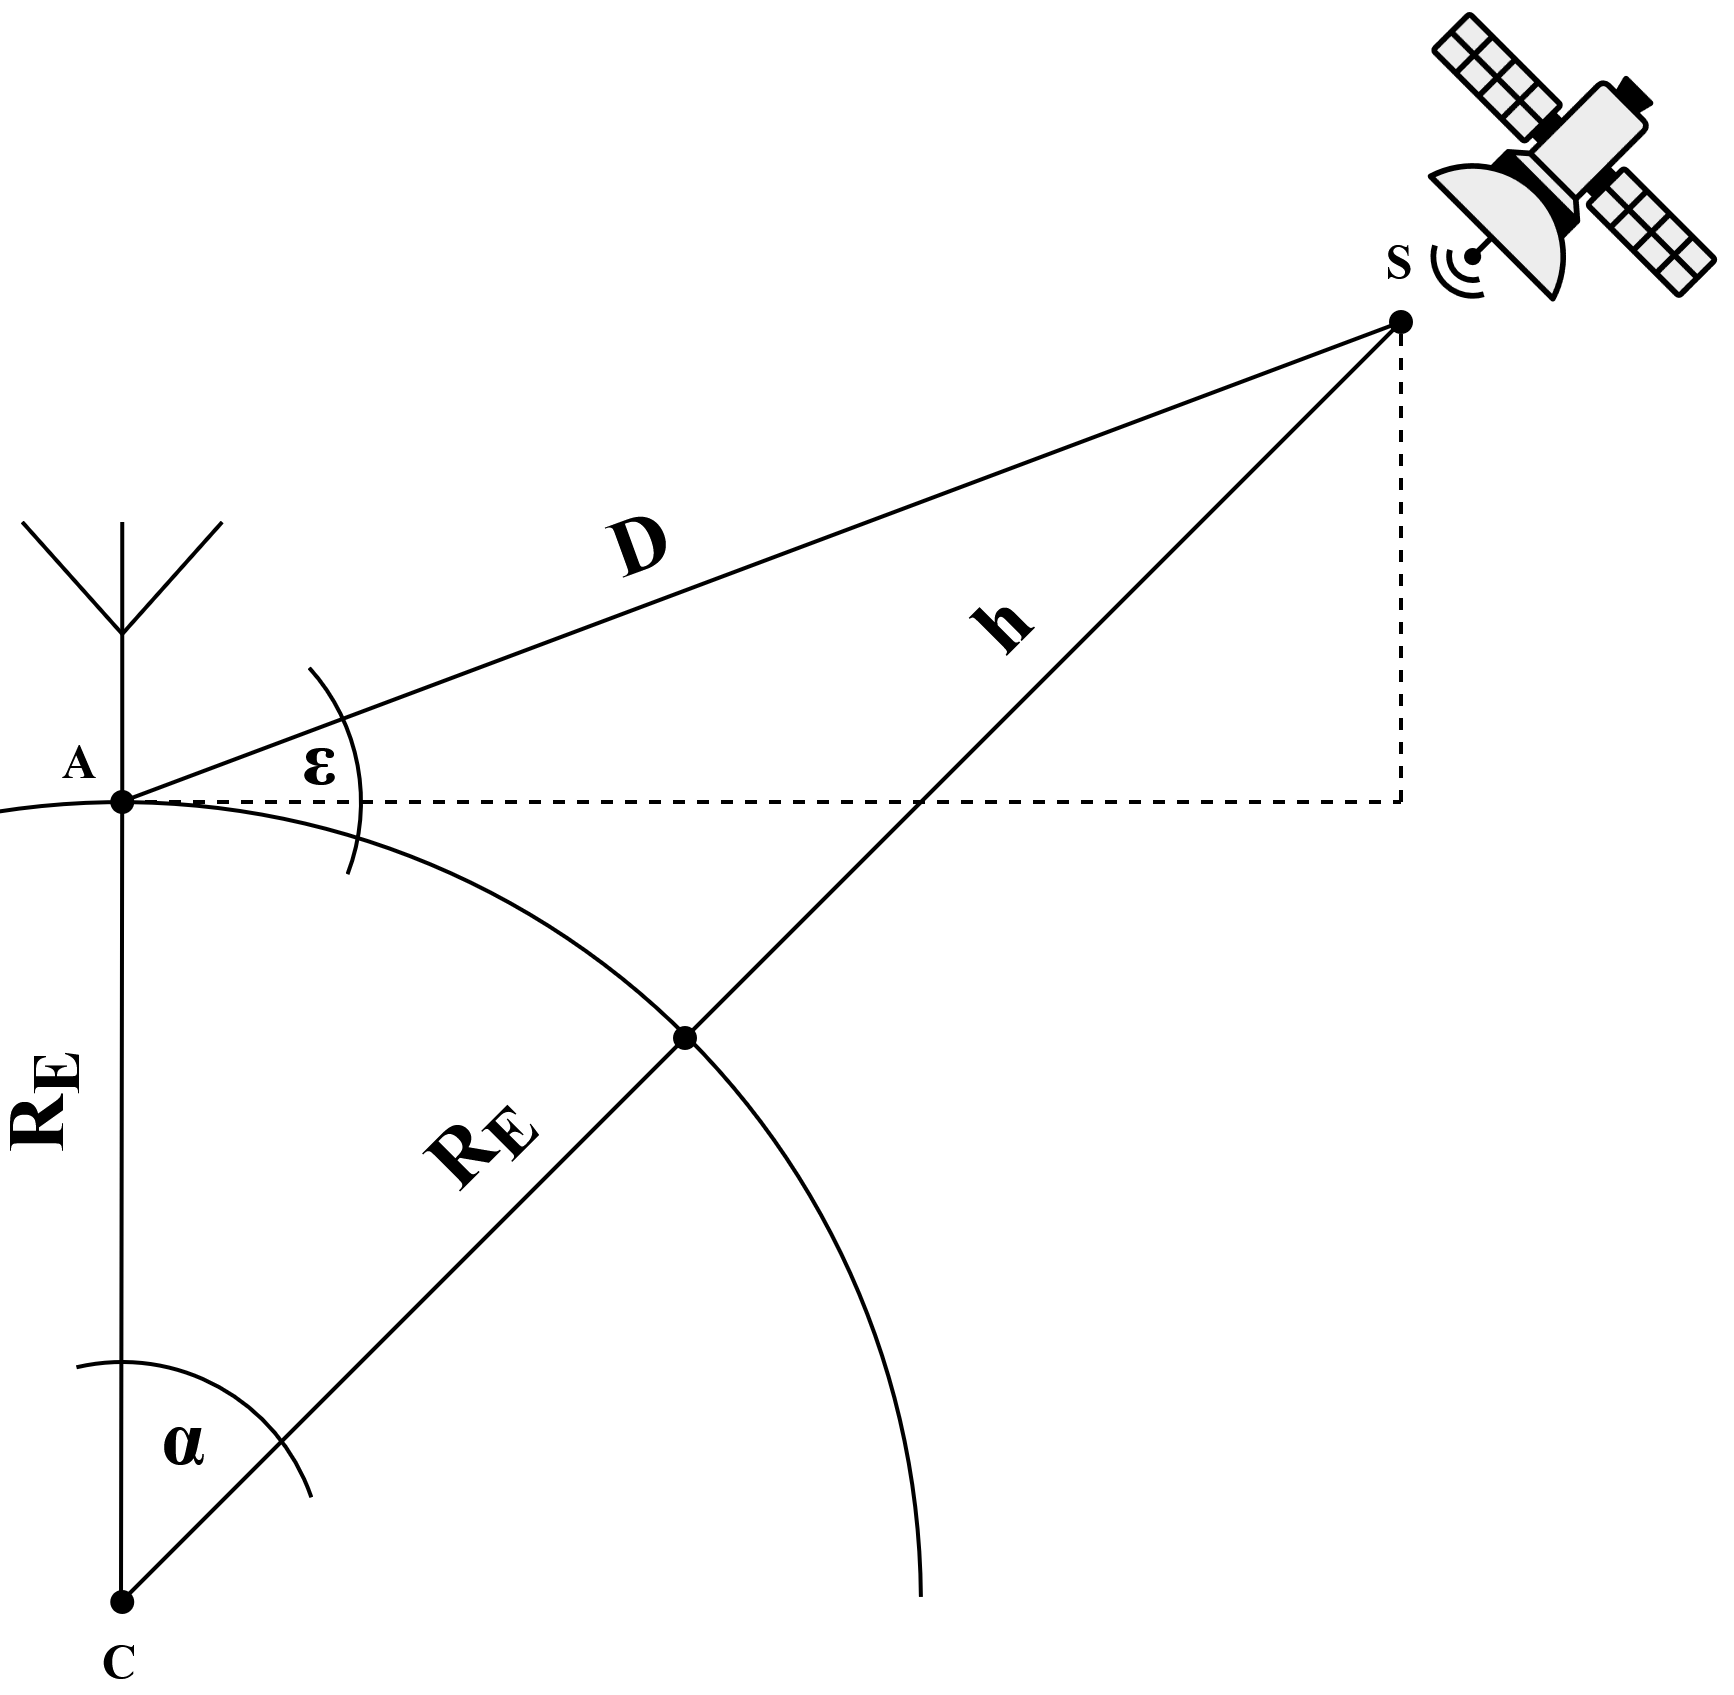
\includegraphics[width=0.6\linewidth]{Figures/07/slant_range.png}
    \caption{Modelo matemático para el cálculo de la distancia D en función del ángulo de elevación $\epsilon$.}
    \label{fig:slant_range}
\end{figure}

Utilizando la ley de los cosenos sobre la geometría esférica de la Tierra, la distancia del enlace se modela rigurosamente como:

\begin{equation}
   (R_E+h)^2 = R_E^2 + d^2 - 2\,R_E\,D\,\cos(\epsilon + \pi/2)
    \label{eq:ley_cos}
\end{equation}

Reemplazando $\cos(\epsilon+\pi/2)$ por $-\text{sen}(\epsilon)$, luego resolviendo la ecuación cuadrática para la variable $D$ y operando matemáticamente se obtiene la expresión:

\begin{equation}
    d(\epsilon) = \sqrt{(R_E + h)^2 - (R_E \cos\epsilon)^2} - R_E \sin\epsilon
    \label{eq:geometria_orbita}
\end{equation}

Como las pérdidas de espacio libre no contemplan efectos disipativos, se deben incluir en el balance de potencias las pérdidas debidas a la atmósfera y las deficiencias mecánicas de apuntamiento de las antenas, factores que, a diferencia de la FSPL, corresponden a pérdidas resistivas reales del trayecto y que se consolidan en la pérdida total de trayecto ($L_{path}$):

\begin{equation}
    L_{path}(\epsilon) \text{ [dB]} = L_{FSPL}(\epsilon) + L_{point} + L_{atm}
    \label{eq:pérdidas_totales}
\end{equation}

Consecuentemente, el nivel de señal recibida (\textit{received signal level}, RSL) en función del ángulo de elevación, análogo a la diferencia entre el EIRP y la pérdida total de trayecto corregida por la ganancia neta de recepción, se determina mediante:

\begin{equation}
    \text{RSL}(\epsilon) \text{ [dBW]} = \text{EIRP} - L_{path}(\epsilon) + G_{rx} - L_{rx}
    \label{eq:rsl_formal}
\end{equation}

% ------------------------------------------------------------------------ %
\subsubsection{Modelado del ruido y calidad del enlace}
La viabilidad del enlace digital no se limita a la amplitud de la portadora recibida, sino a su relación respecto a la densidad espectral de potencia de ruido térmico presente en el sistema ($N_0$), modelado como ruido blanco gaussiano aditivo. En sistemas terrestres, este ruido suele caracterizarse mediante la figura de ruido del receptor referida a una temperatura estándar de 290\,K, sin embargo, en estaciones terrenas de comunicaciones satelitales la antena recibe directamente el ruido de cielo, sustancialmente menor a 290\,K, por lo cual resulta más preciso emplear una temperatura total de sistema en lugar de una figura de ruido equivalente. Bajo este criterio, la temperatura total de ruido del sistema receptor ($T_{sys}$) se descompone aditivamente de acuerdo con el teorema de uniones en cascada, simplificado para los componentes críticos del segmento terreno:

\begin{equation}
    T_{sys} = T_{ant} + T_{LNA}
    \label{eq:tsys}
\end{equation}

donde $T_{ant}$ es la temperatura de ruido equivalente de la antena, que captura la radiación de fondo cósmico y el ruido térmico terrestre captado por los lóbulos secundarios, y $T_{LNA}$ es la temperatura de ruido efectiva referida a la entrada del amplificador de bajo ruido. La densidad espectral de ruido resultante se expresa logarítmicamente como:

\begin{equation}
    N_0 \text{ [dBW/Hz]} = k_{dB} + 10 \log_{10}(T_{sys})
    \label{eq:n0_log}
\end{equation}

donde $k_{dB} = -228{,}6 \text{ dBW/(K}\cdot\text{Hz)}$ es la expresión logarítmica de la constante de Boltzmann.

La evaluación final del desempeño del enlace digital requiere la determinación de la relación entre energía de bit disponible y densidad espectral de ruido ($E_b/N_0$), la cual se obtiene dividiendo la potencia de señal por la tasa de bits para obtener la energía por bit ($E_b = S/R_b$) y la potencia de ruido total por el ancho de banda equivalente para obtener la densidad espectral ($N_0 = N/B$), de modo que $E_b/N_0 = (S/N)(B/R_b)$. En términos del balance de enlace ya formulado, esta relación disponible en función del ángulo de elevación se expresa como:

\begin{equation}
    \frac{E_b}{N_0}(\epsilon) \text{[dB]} = \text{RSL}(\epsilon) - N_0 - 10\log_{10}(R_b)
    \label{eq:ebn0_rb}
\end{equation}

donde el único parámetro de la cadena de transmisión digital que interviene en la ecuación es la tasa de bits $R_b$, con independencia de cómo esta haya sido determinada. En sistemas con asignación espectral rígida, $R_b$ no constituye un parámetro libre sino una cantidad derivada del ancho de banda ocupado ($BW$) y de las características del esquema de modulación. La tasa de símbolos (\textit{symbol rate}, $R_s$) en baudios se deduce a partir del factor de roll-off $\alpha$ del filtro de coseno realzado empleado para conformar el espectro, dado que la relación entre el ancho de banda ocupado y la tasa de símbolos para este tipo de filtrado responde a:

\begin{equation}
    R_s = \frac{BW}{1 + \alpha}
    \label{eq:rs_bw}
\end{equation}

A partir de la eficiencia espectral del esquema de modulación lineal M-PSK implementado, la tasa de bits efectiva queda determinada por la cantidad de bits por símbolo ($\log_{2}M$):

\begin{equation}
    R_b = R_s \log_{2}(M) = \frac{BW}{1 + \alpha} \log_{2}(M)
    \label{eq:rb_deducido}
\end{equation}

de modo que, bajo un ancho de banda constante, el aumento en el orden de la modulación $M$ incrementa la tasa de transmisión a costa de una reducción proporcional en el $E_b/N_0$ disponible por bit, según se desprende de sustituir \eqref{eq:rb_deducido} en \eqref{eq:ebn0_rb}.

El valor de $[E_b/N_0]_{req}$ que interviene en el criterio de cierre del enlace no es un parámetro arbitrario, sino que depende exclusivamente de dos factores: el esquema de modulación digital empleado y la tasa de error de bit (BER) objetivo de la misión. Esta dependencia se establece a través de la función de error complementaria gaussiana, comúnmente expresada mediante la función $Q(z)$, que es la herramienta analítica para poder vincular la relación señal a ruido disponible con la probabilidad de error de detección en presencia de ruido.

\begin{equation}
    Q(z) = \frac{2}{\sqrt{\pi}} \int_{z}^{\infty} e^{-t^2}\, dt
    \label{eq:funcion_q}
\end{equation}

Para un esquema de modulación M-PSK sujeto a detección coherente sobre un canal de ruido blanco gaussiano aditivo, la tasa de error de bit puede aproximarse en función de $E_b/N_0$ mediante:

\begin{equation}
    \text{BER} \approx \frac{2}{\log_{2}(M)}\, Q\!\left( \sqrt{2 \log_{2}(M)} \, \sin\!\left(\frac{\pi}{M}\right) \sqrt{\frac{E_b}{N_0}} \right)
    \label{eq:ber_mpsk}
\end{equation}

expresión que, al ser invertida numéricamente para una BER objetivo preestablecida, permite obtener el valor de $[E_b/N_0]_{req}$ correspondiente a cada orden de modulación $M$. De esta manera, modulaciones de mayor orden, que ofrecen una mayor eficiencia espectral al transmitir más bits por símbolo, exigen simultáneamente una relación $E_b/N_0$ más elevada para sostener la misma tasa de error, lo cual constituye el compromiso fundamental entre velocidad de transmisión y robustez frente al ruido que se evalúa a lo largo de este balance de enlace.

Para asegurar la robustez del enlace ante desvanecimientos repentinos o imprecisiones, el margen operativo instantáneo $M_{arg}(\epsilon)$ frente al requerimiento teórico de la modulación empleada ($[E_b/N_0]_{req}$) debe superar un umbral mínimo preestablecido ($M_{min}$):

\begin{equation}
    M_{arg}(\epsilon) = \frac{E_b}{N_0}(\epsilon) - [E_b/N_0]_{req} \ge M_{min}
    \label{eq:margen}
\end{equation}

El cumplimiento de esta desigualdad define analíticamente el ángulo de elevación mínimo de visibilidad operativa $\epsilon_{min}$, por debajo del cual el enlace se considera no viable para la comunicación con la modulación correspondiente.

% ------------------------------------------------------------------------ %
\subsubsection{Implementación computacional y simulación}
Con el propósito de validar los rangos de operación del amplificador de potencia diseñado y determinar los límites físicos de la comunicación, se desarrollaron dos scripts en lenguaje Python~\cite{python} que implementan las ecuaciones~\eqref{eq:eirp_analitico} a \eqref{eq:margen}, utilizando interfaces gráficas interactivas basadas en la biblioteca Tkinter~\cite{tkinter} e integración de cálculo numérico vectorizado con NumPy~\cite{numpy} y visualización mediante Matplotlib~\cite{matplotlib}.

El primer programa desarrollado evalúa la viabilidad del enlace configurando la tasa de bits. El script barre los valores del ángulo de elevación $\epsilon \in [0^\circ, 90^\circ]$ y calcula, mediante la ecuación~\eqref{eq:ebn0_rb}, una única curva de $E_b/N_0$ disponible en función de la elevación. Dado que la tasa de bits es común a todo el sistema, esta misma curva se contrasta simultáneamente contra los tres umbrales requeridos ($[E_b/N_0]_{req}$ de QPSK, 8-PSK y 16-PSK), determinando para cada modulación el primer índice angular que satisface el criterio de cierre de la ecuación~\eqref{eq:margen}.

El segundo script refina el análisis tomando como variables de entrada el ancho de banda ocupado en radiofrecuencia (BW) y el factor de roll-off del filtro ($\alpha$), a partir de los cuales calcula una tasa de símbolos común mediante la ecuación~\eqref{eq:rs_bw} y, posteriormente, obtiene la tasa de bits específica de cada esquema de modulación, multiplicando dicha tasa de símbolos por la cantidad de bits por símbolo correspondiente, de acuerdo con la ecuación~\eqref{eq:rb_deducido}. Sustituyendo esta expresión de $R_b$ en función del ancho de banda dentro de la ecuación~\eqref{eq:ebn0_rb}, se obtiene la relación de $E_b/N_0$ empleada por este segundo script:

\begin{equation}
    \frac{E_b}{N_0}(\epsilon) \text{ [dB]} = \text{RSL}(\epsilon) - N_0 - 10\log_{10}\left(\frac{BW}{1+\alpha}\log_{2}(M)\right)
    \label{eq:ebn0_bw}
\end{equation}

Debido a que en este caso cada modulación posee su propia tasa de bits y, en consecuencia, su propia curva de $E_b/N_0$ disponible en función de la elevación, calculada de forma independiente mediante la ecuación~\eqref{eq:ebn0_bw}, el resultado son tres curvas diferenciadas, y no una curva única contrastada contra tres umbrales, lo cual modela fielmente el compromiso entre el orden de la modulación, la velocidad de transmisión resultante y la degradación del margen disponible frente al ruido térmico.

Los parámetros de simulación nominales cargados por defecto en ambas herramientas informáticas, representativos de la arquitectura física del CubeSat y el segmento terreno en banda S, se consolidan en el Cuadro~\ref{tab:parametros_scripts}.

\begin{table}[H]
    \centering
    \caption{Parámetros de diseño y simulación empleados en los scripts de cálculo de radioenlace.}
    \label{tab:parametros_scripts}
    \begin{tabular}{lccc}
        \hline\hline
        \textbf{Parámetro del Sistema}      & \textbf{Símbolo} & \textbf{Valor}  & \textbf{Unidad} \\
        \hline
        Frecuencia de Operación             & $f$              & 2,2             & GHz  \\
        Radio de Órbita Satelital           & $h_{orb}$        & 600             & km   \\
        Ancho de Banda de Canal             & $BW$             & 2,0             & MHz  \\
        Factor de Roll-off                  & $\alpha$         & 0,35            & ---  \\
        Tasa de Bits de Referencia          & $R_b$            & 3               & Mbps \\
        Potencia de Salida del Transmisor   & $P_t$            & 0,0             & dBW  \\
        Pérdidas en el Transmisor           & $L_{tx}$         & 1,0             & dB   \\
        Ganancia de la Antena Transmisora   & $G_{tx}$         & 7,0             & dBi  \\
        Pérdidas por Apuntamiento de Antena & $L_{point}$      & 1,0             & dB   \\
        Pérdidas por Atenuación Atmosférica & $L_{atm}$        & 1,0             & dB   \\
        Ganancia de la Antena Receptora     & $G_{rx}$         & 27,0            & dBi  \\
        Pérdidas en el Sistema Receptor     & $L_{rx}$         & 1,0             & dB   \\
        Temperatura de Antena               & $T_{ant}$        & 55              & K    \\
        Temperatura de Ruido del LNA        & $T_{LNA}$        & 70             & K    \\
        Margen Establecido                  & $M_{min}$        & 1,0             & dB   \\
        \hline\hline
    \end{tabular}
\end{table}

A continuación, las Figuras~\ref{fig:grafico_bitrate} y \ref{fig:grafico_bw} ilustran las curvas de desempeño obtenidas mediante las interfaces gráficas implementadas para cada una de las metodologías analizadas.

\begin{figure}[H]
    \centering
    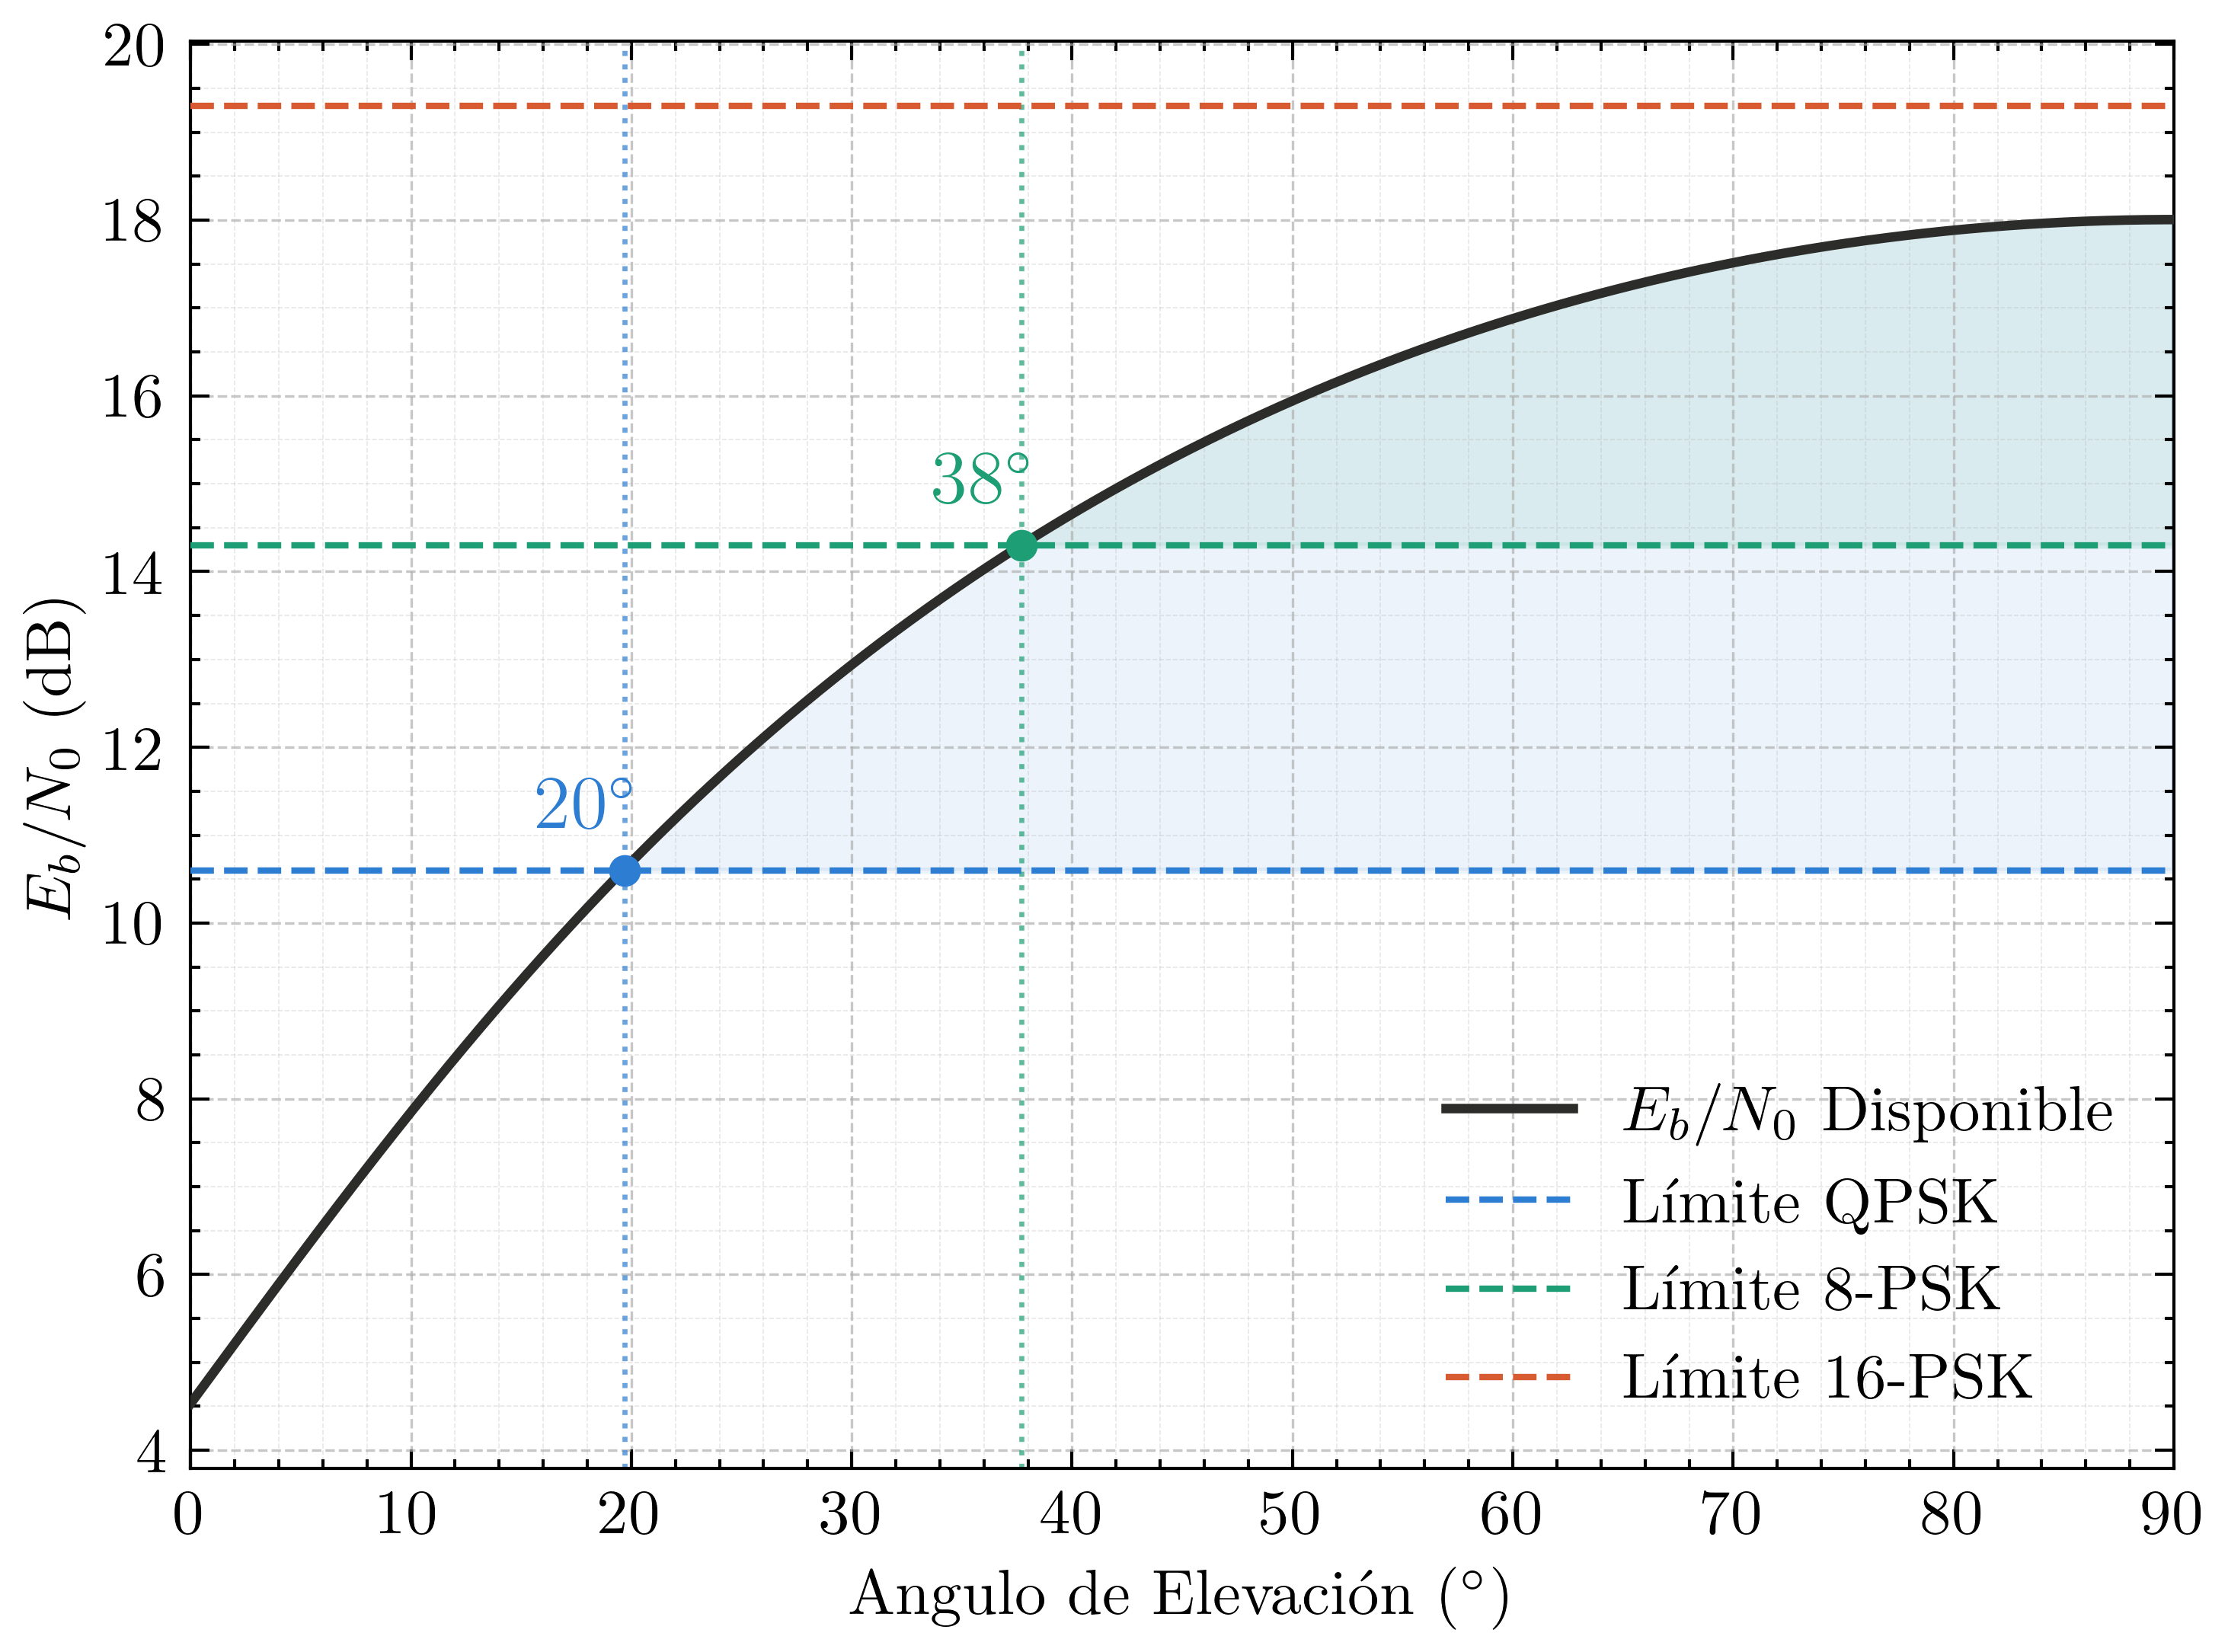
\includegraphics[width=0.8\linewidth]{Figures/07/lb_rb_plot.png}
    \caption{Curva de $E_b/N_0$ disponible frente a elevación para una tasa de bits constante ($R_b = 3\text{Mbps}$).}
    \label{fig:grafico_bitrate}
\end{figure}

\begin{figure}[H]
    \centering
    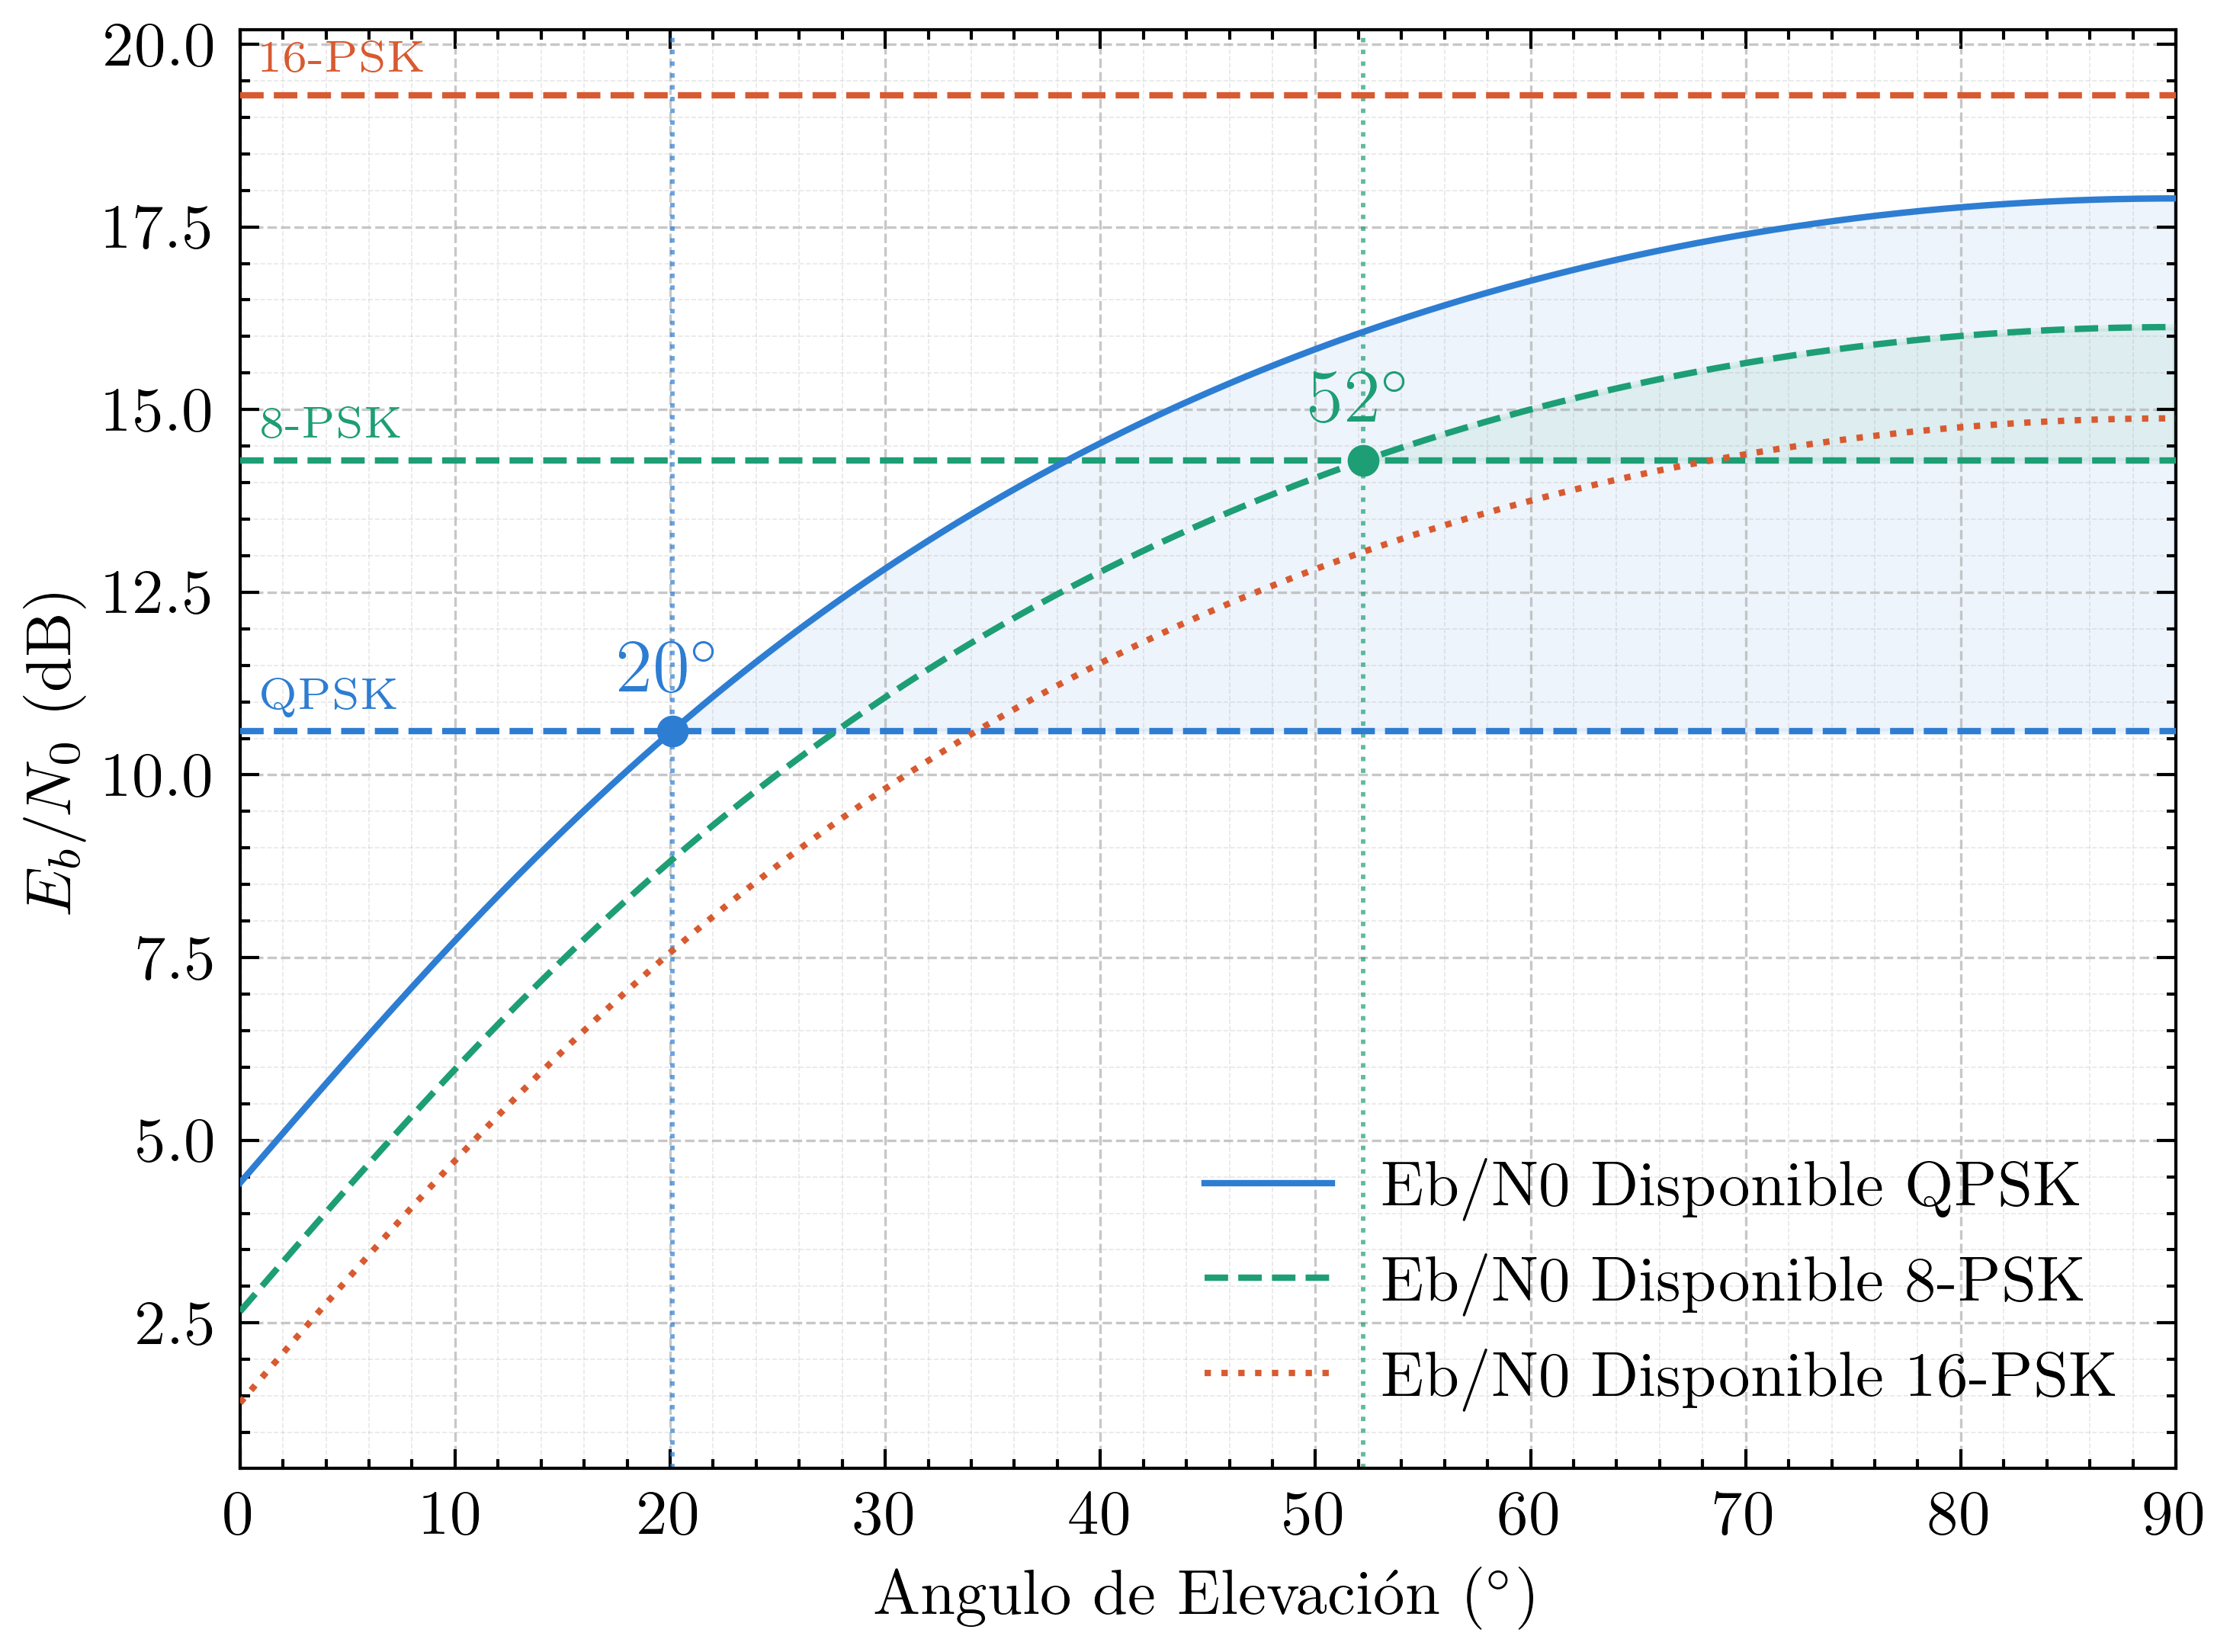
\includegraphics[width=0.8\linewidth]{Figures/07/lb_bw_plot.png}
    \caption{Curvas diferenciadas de $E_b/N_0$ disponible por modulación para un ancho de banda fijo ($BW = 2\text{ MHz}$).}
    \label{fig:grafico_bw}
\end{figure}

El Cuadro~\ref{tab:parametros_scripts} reporta el valor de $R_b$ empleado en la Figura~\ref{fig:grafico_bitrate}, obtenida mediante el primer script a tasa de bits constante, y el valor de $BW$ empleado en la Figura~\ref{fig:grafico_bw}, obtenida mediante el segundo script a ancho de banda constante. Ambas figuras coinciden en el ángulo de elevación mínimo requerido por QPSK, de aproximadamente $20^\circ$, dado que a esta modulación le corresponde, en ambos casos, prácticamente el mismo par de valores de $R_b$ y $BW$. Para 8-PSK y 16-PSK, en cambio, cada figura impone una condición distinta sobre el sistema, y los ángulos de cierre difieren entre ambas.

En el primer script, con $R_b=3~\,Mbps$ constante, no se consideró el factor de roll-off $\alpha$. En consecuencia, el ancho de banda mínimo asociado a cada modulación bajo este escenario se obtiene directamente a partir de la tasa de símbolos $R_s = R_b/\log_2(M)$, sin el margen adicional que introduce el filtrado de coseno realzado, lo que arroja $BW \approx 1,50~\,MHz$ para QPSK, $BW \approx 1,00~\,MHz$ para 8-PSK y $BW \approx 0,75~\,MHz$ para 16-PSK. Cabe notar que estos valores no resultan directamente comparables con el ancho de banda de canal $BW=2~\,MHz$ del Cuadro~\ref{tab:parametros_scripts}, dado que dicho valor de referencia sí incorpora el margen de roll-off propio del segundo script, mientras que la ecuación~\eqref{eq:bw_despejado} refleja únicamente el ancho de banda de Nyquist mínimo requerido por cada modulación bajo el criterio de tasa de bits constante.

De manera análoga, con $BW = 2\text{ MHz}$ constante, la tasa de bits que resulta para cada modulación se obtiene de la ecuación~\eqref{eq:rb_deducido}, empleando la tasa de símbolos de la ecuación~\eqref{eq:rs_bw}, lo que arroja $R_b \approx 2,96~\,Mbps$ para QPSK, $R_b \approx 4,44~\,Mbps$ para 8-PSK y $R_b \approx 5,93~\,Mbps$ para 16-PSK. En este caso, a igual ancho de banda, un orden de modulación mayor permite transmitir a una tasa de bits considerablemente más elevada, a costa de exigir una relación $E_b/N_0$ mayor para sostener la misma tasa de error, según se desprende de la ecuación~\eqref{eq:ber_mpsk}.

De la comparación entre ambas figuras se desprende que 16-PSK no resulta viable para el enlace bajo los parámetros nominales del Cuadro~\ref{tab:parametros_scripts} en ninguno de los dos escenarios analizados. Con $R_b$ constante el $E_b/N_0$ disponible en el punto de máxima elevación alcanza aproximadamente $18,0~\,dB$, frente a un requerimiento $E_b/N_0_{req}$ de aproximadamente $19,4~\,dB$ para 16-PSK. Con $BW$ constante, la diferencia entre el valor requerido y el obtenido es aún mayor dado que sostener 16-PSK a ancho de banda fijo exige una tasa de bits considerablemente mayor que la empleada por QPSK y 8-PSK, lo cual penaliza directamente al $E_b/N_0$ disponible según la ecuación~\eqref{eq:ebn0_bw}.

Cerrar el enlace con 16-PSK requiere incrementar el margen disponible. Este incremento podría obtenerse mediante un aumento equivalente en la ganancia de la antena transmisora o receptora, mediante una reducción de la temperatura de ruido del sistema receptor $T_{sys}$ empleando un amplificador de bajo ruido de menor figura de ruido, o bien, en el escenario de $R_b$ constante, reduciendo directamente la tasa de bits objetivo. Cabe destacar que cualquiera de estas mejoras del presupuesto de enlace no beneficia exclusivamente a 16-PSK, sino que se traslada directamente a QPSK y a 8-PSK en forma de un mayor margen operativo o de un ángulo de elevación mínimo de cierre más reducido, ampliando la fracción de cada pasada satelital disponible para la comunicación.

Sin embargo, cada una de estas alternativas conlleva un compromiso propio. Incrementar la ganancia de antena, tanto en el segmento espacial como en el terreno, implica típicamente aumentar sus dimensiones físicas o su directividad, lo cual resulta particularmente restrictivo para la antena del CubeSat dado el presupuesto de masa y de volumen impuesto por el formato, según se discutió en el Capítulo~\ref{chap:cubesat_leo}. Reducir $T_{sys}$ mediante un amplificador de bajo ruido de mejor figura de ruido incrementa el costo y la complejidad del segmento terreno, sin afectar al segmento espacial, pero sin representar una mejora atribuible al diseño del amplificador de potencia desarrollado en este trabajo. Finalmente, reducir la tasa de bits objetivo para viabilizar 16-PSK resulta contradictorio con la motivación original de emplear una modulación de mayor orden, dado que dicha motivación reside precisamente en alcanzar una mayor tasa de transmisión o, alternativamente, un menor ancho de banda ocupado para una tasa de bits dada, tal como se cuantificó en los párrafos anteriores. En consecuencia, para el amplificador de potencia desarrollado, QPSK y 8-PSK constituyen los esquemas de modulación M-PSK viables dentro del rango de elevación de una pasada satelital típica, mientras que 16-PSK requeriría una mejora adicional del presupuesto de enlace, ajena al desempeño del amplificador de potencia en sí, para resultar viable.
\include{Chapters/08-Resultados.tex}
\chapter[Conclusiones]{Conclusiones} \label{cp:conclusiones}

A lo largo de este trabajo se abordó el diseño, la simulación, la fabricación y la caracterización experimental de un amplificador de potencia Clase AB en banda S para aplicaciones de enlace descendente en CubeSats, junto con un acoplador híbrido en cuadratura concebido como primera etapa hacia una futura arquitectura Doherty. El desarrollo completo, desde el marco teórico hasta la medición de los prototipos fabricados, permitió recorrer la totalidad del proceso de diseño de un sistema de RF para aplicaciones espaciales, contemplando tanto las restricciones propias de cada circuito como las impuestas por la plataforma CubeSat y por el entorno de órbita baja terrestre.

El acoplador híbrido en cuadratura, implementado mediante una topología de línea ramificada plegada para reducir sus dimensiones, alcanzó en su segunda versión una frecuencia central de 2,019~GHz y un desfasaje de 92,57° entre los puertos de salida en la frecuencia de interés, valores considerablemente más próximos al comportamiento ideal que los obtenidos con la primera versión fabricada. Esta mejora entre versiones validó de manera directa la hipótesis formulada durante el proceso de diseño, según la cual el corrimiento de frecuencia observado se debía a la falta de modelado de la transición hacia el conector SMA, y confirmó la utilidad de la verificación electromagnética de onda completa como herramienta de diagnóstico frente a las limitaciones del modelo esquemático de líneas de transmisión ideales. La comparación entre los resultados medidos y los obtenidos mediante simulación en ADS y en CST mostró, además, una concordancia satisfactoria entre ambas plataformas de simulación y el prototipo fabricado, con una mayor precisión de CST atribuible a su capacidad de capturar los efectos parásitos de la geometría real del layout.

El amplificador de potencia, por su parte, cumplió con los requisitos mandatorios de ancho de banda, potencia de salida y OIP3 establecidos en el anteproyecto, alcanzando un ancho de banda de 70~MHz, una potencia de salida de 30,92~dBm en las proximidades del P1dB y un OIP3 de 39,83~dBm. Los parámetros que no llegaron a satisfacer plenamente el objetivo de diseño, la frecuencia central y la PAE, resultaron sin embargo muy próximos a dicho objetivo: la frecuencia central medida de 2,11~GHz se ubicó a solo 90~MHz del valor de diseño de 2,2~GHz, mientras que la PAE de 30,51\,\% obtenida en las proximidades del P1dB se aproximó de manera considerable al 35\,\% especificado, incluso superándolo al operar el amplificador dentro de su región de compresión. Cabe destacar que dichos objetivos de diseño fueron originalmente formulados pensando en una arquitectura Doherty completa, compuesta por un amplificador de portadora y un amplificador de pico operando en conjunto, y no en un único amplificador Clase AB operando de manera aislada como el desarrollado a partir de la redefinición de alcance descripta en el Capítulo~\ref{sec:alcance}. Que un amplificador Clase AB simple haya logrado aproximarse en tal medida a especificaciones concebidas para una topología de mayor complejidad y de mayor eficiencia constituye un resultado alentador de cara a una futura implementación Doherty completa, en la cual cabe esperar que la combinación de ambas ramas de amplificación permita satisfacer los objetivos no alcanzados y superar holgadamente los que ya fueron cumplidos.

De manera análoga a lo observado en el acoplador, la comparación entre los resultados medidos y los simulados en ADS a nivel esquemático evidenció el origen de las principales discrepancias del amplificador, atribuidas a la inductancia parásita de los componentes discretos de la red de estabilidad y a una resonancia fuera de banda no capturada por el modelo esquemático original. La identificación puntual de estas causas a través de un proceso de análisis similar al del acoplador deja establecidas dos mejoras concretas y directamente accionables para una futura iteración del diseño: la incorporación de la inductancia equivalente serie de los componentes de la red de estabilidad desde las primeras etapas de simulación y un modelado más detallado de los efectos parásitos del layout físico y del empaquetado de los componentes.

El trabajo futuro cuenta con un conjunto de mejoras ya identificadas y fundamentadas que permitirían acercar aún más el desempeño de ambos circuitos a sus respectivos comportamientos ideales. Para el acoplador, como fue mencionado en la Sección~\ref{sec:resultados_acoplador}, un cambio de sustrato dieléctrico permitiría reducir aún más sus dimensiones físicas, mientras que la incorporación de un modelo tridimensional del conector SMA en la simulación electromagnética permitiría reducir la discrepancia entre los resultados simulados y los medidos. La asimetría observada entre los parámetros de reflexión de los puertos de salida del acoplador, sin una explicación igualmente clara hasta el momento, constituye asimismo un aspecto que amerita un estudio más profundo. Para el amplificador, además de las mejoras de modelado ya mencionadas, el análisis de radioenlace desarrollado en la Sección~\ref{sec:radioenlace} estableció que un incremento del margen disponible, ya sea mediante una mayor ganancia de antena o mediante una reducción de la temperatura de ruido del sistema receptor, habilitaría el empleo de esquemas de modulación de mayor orden, mejora que además beneficiaría de manera directa a los esquemas QPSK y 8-PSK ya viables, ampliando el margen operativo y la fracción de cada pasada satelital disponible para la comunicación.

Naturalmente, la continuación más significativa de este trabajo reside en completar la arquitectura Doherty originalmente planteada, incorporando el amplificador de pico y la red de combinación de salida correspondiente. El acoplador desarrollado y caracterizado en este trabajo se encuentra ya en condiciones de cumplir su función como red de división de señal de entrada en dicha arquitectura, mientras que el amplificador Clase AB caracterizado puede ser directamente reutilizado como amplificador de portadora del sistema Doherty completo. En este sentido, ambos desarrollos presentados no constituyen resultados aislados, sino los dos primeros bloques constitutivos de un sistema de mayor complejidad, cuya continuación resulta ampliamente respaldada por el desempeño individual alcanzado por cada uno.

Finalmente, más allá de los resultados técnicos particulares de cada circuito, este trabajo permitió atravesar de manera integral las etapas propias del desarrollo de un módulo de radiofrecuencia para aplicaciones espaciales, desde el diseño teórico y la simulación asistida por computadora hasta la fabricación de circuitos impresos y la caracterización experimental en laboratorio, incluyendo la articulación con instituciones externas para acceder a instrumental de medición especializado no disponible en la institución de origen. La necesidad de redefinir el alcance original del proyecto debido a restricciones de tiempo, costo y disponibilidad de equipamiento constituyó un aprendizaje relevante sobre la gestión de un proyecto de ingeniería real, en el cual las condiciones planteadas rara vez coinciden exactamente con la planificación inicial. La plataforma de diseño, simulación y caracterización desarrollada y validada a lo largo de este trabajo, junto con el conjunto de mejoras concretas identificadas para su continuación, sienta una base sólida y reutilizable para el desarrollo de futuros módulos de radiofrecuencia orientados a aplicaciones aeroespaciales.

%%% Bibliography %%%
\renewcommand{\refname}{Bibliografía}
\printbibliography[title={\refname},heading=bibintoc]

%%% Appendices: Work that *YOU* Developed %%%
\appendix
\input{Matter/06-Appendices}
\chapter{Procesamiento de datos con Python} \label{appendix:python_scripts}


\chapter{Procesamiento de incertidumbre con Python} \label{appendix:uncertainty_script}

 
%%% Back Page %%%
\input{Matter/08-Back-Page}

\end{document}